\documentclass[a4paper]{article}
\usepackage[margin=2.7cm]{geometry}
\usepackage{graphicx} % Required for inserting images
\usepackage{tcolorbox}
\usepackage{amsfonts}
\usepackage{amsthm}
\usepackage{amsmath}
\usepackage[italian]{babel}
\usepackage{csquotes}
\usepackage{multicol}
\usepackage{tikz}
\usepackage{tikz-cd}
\usepackage{wrapfig}
\usepackage{enumitem}
\usepackage{awesomebox}
\usepackage[dvipsnames]{xcolor}
\usepackage{soul}
\usepackage{cancel}
\usepackage{mathtools}
\usepackage[bookmarks, hidelinks]{hyperref}
\newcommand{\mathcolorbox}[2]{\colorbox{#1}{$\displaystyle #2$}}
\newcommand{\hlfancy}[2]{\sethlcolor{#1}\hl{#2}}
\newcommand{\IM}{\ \mathrm{Im} \ }
\usepackage{fancyhdr}

\setlist[description]{leftmargin=\parindent,labelindent=\parindent}
\tcbuselibrary{theorems, skins}

\newtcbtheorem[number within=section,list inside={teo}]{teo}{Teorema}
{enhanced, coltitle=green!35!black, fonttitle=\bfseries,
                                colbacktitle=green!10, colback=green!12,
                                frame hidden, boxrule=0pt,
                                attach title to upper={\\[0.5ex]}, 
                                borderline west={1mm}{-2mm}{green!35!black}}
{th}
\theoremstyle{definition}
\newtcbtheorem[number within=section,list inside={cor}]{cor}{Corollario}
{enhanced, coltitle=orange!35!black, fonttitle=\bfseries,
                                colbacktitle=orange!10, colback=orange!10,
                                frame hidden, boxrule=0pt,
                                attach title to upper={\\[0.5ex]}, 
                                borderline west={1mm}{-2mm}{orange!35!black}}
{th}
\newtcbtheorem[number within=section,list inside={deff}]{deff}{Definizione}
{enhanced, coltitle=blue!25!black, fonttitle=\bfseries,
								colbacktitle=blue!10, colback=blue!5,
								frame hidden, boxrule=0pt,
								attach title to upper={\\[0.5ex]}, 
								borderline west={1mm}{-2mm}{blue!25!gray}}
{th}
\newtheorem*{oss}{Osservazione}
\newtheorem*{es}{Esempio}
\newtheorem*{prop}{Proposizione}

\title{Appunti Algebra e Geometria}
\author{Maicol Battistini}

\begin{document}

\maketitle
\tableofcontents
\newpage

\tcblistof[\section*]{deff}{Lista delle definizioni}
\tcblistof[\section*]{teo}{Lista dei teoremi}
\tcblistof[\section*]{cor}{Lista dei corollari}

\newpage

\pagestyle{fancy}
\fancyhead[lo]{\nouppercase{\rightmark}}
\fancyhead[ro,le]{\thepage}

\section{Unità 1 - Lezioni 1, 2}
\subsection{Insiemi}
\begin{deff}{Relazione di un insieme}{}
	Una relazione su un insieme \(A\) è un sottoinsieme \(R\) di \(A \times A\). \\
	Scrivo \(a_1 \ R \ a_2\) se \( (a_1, a_2) \in R\) e dico\enquote*{\(a_1\) è in relazione con \(a_2\)}
\end{deff}
\begin{deff}{Relazione di equivalenza}{}
	Una relazione \(R\) è una relazione di equivalenza se valgono le seguenti proprietà:
	\begin{description}
		\item \textbf{Riflessiva}: \(a \ R \ a \ \forall a \in A \)
		\item \textbf{Simmetrica}: \(a \ R \ b \ \Rightarrow b \ R \ A \)
		\item \textbf{Transitiva}: \(a \ R \ a, b \ R \ c \ \Rightarrow a \ R \ c \)
	\end{description}
\end{deff}
\begin{deff}{Congruenza}{}
	\[ \mathbb{Z} = {0, 1, -1, 2, -2, 3, -3, ...} \]
	Sia $n \in \mathbb{Z}, n >= 2$
	\begin{align*}
		a \equiv b \ (n) &  & \text{\enquote*{$a$ è congruo a $b$ modulo $n$}}
	\end{align*}
	se $a - b$ è multiplo di $n$ (cioè $\exists h \mid a - b = hn$)
\end{deff}
Esempi:
\begin{align*}
	8 \equiv 23 (5) &  & 8 \not\equiv 17(5) &  & 4 \equiv 10,16,-2,-8(6) &  & 4 \not\equiv 13(6)
\end{align*}
\begin{oss}
	Essere congrui modulo n è una relazione di equivalenza
\end{oss}
\begin{proof}
	Dimostro le tre proprietà della relazione di equivalenza:
	\begin{description}
		\item Riflessiva: \[ \forall a \in \mathbb{Z}, \ a \equiv a (n) \ \text{perchè} \ a - a = 0 = 0 \cdot n\]
		\item Simmetrica: \\ se $a \equiv b (n)$, allora $b \equiv a (n)$ perchè se $a - b = hn \Rightarrow b - a = -hn$
		\item Transitiva: \\ se $a \equiv b (n)$ e $b \equiv c (n)$, allora $a \equiv c (n)$ perchè se $a - b = hn$ e $b - c = kn$, allora $a - c = (a - b) + (b - c) = (h + k)n$
	\end{description}
\end{proof}
\subsection{Funzioni e applicazioni}
\[ f: X \rightarrow Y \]
\[ f(a) = b \]

$f$ è una applicazione se ad ogni $a \in X$ corrisponde uno e un solo $b \in Y$

\begin{deff}{Funzione iniettiva}{}
	Una funzione $f: X \rightarrow Y$ è iniettiva se:
	\[ \forall x_1, x_2 \in X \mid x_1 = x_2 \Rightarrow f(x_1) = f(x_2) \]
	Ovvero: \enquote*{due elementi distinti di $X$ vengono mandati in elementi distinti di $Y$}
	\begin{center}
		\includegraphics{images/iniettiva.png}
	\end{center}
\end{deff}
\begin{deff}{Funzione suriettiva}{}
	Una funzione $f: X \rightarrow Y$ è suriettiva se:
	\[
		Y = Im \ f = \{y \in Y \mid \exists x \in X \mid f(x) = y\}
	\]
	Ovvero: \enquote*{ogni elemento di $Y$ è immagine di almeno un elemento di $X$}
	\begin{center}
		\includegraphics{images/suriettiva.png}
	\end{center}
\end{deff}
\begin{deff}{Funzione biunivoca}{}
	Una funzione $f: X \rightarrow Y$ è biunivoca se è iniettiva e suriettiva, cioè se per ogni $y \in Y$ esiste un solo $x \in X$ tale che $f(x) = y$
	\begin{center}
		\includegraphics{images/biunivoca_1.png}
	\end{center}
	\begin{es}
		Una funzione biunivoca è invertibile, cioè $\exists f^{-1}: Y \rightarrow X$ tale che $f^{-1} \circ f = Id_X$ e $f \circ f^{-1} = Id_Y$
	\end{es}
	\begin{center}
		\includegraphics{images/biunivoca_2.png}
	\end{center}
\end{deff}
\begin{es}
	\[ f_1: \mathbb{R} \rightarrow \mathbb{R}, f(1) = x^2 \]
	\begin{description}
		\item Iniettiva? No, perchè $f(-1) = f(1) = 1$
		\item Suriettiva? No, perchè $Im \ f = \{y \in \mathbb{R} \mid y \ge 0\} \ne \mathbb{R}$
		\item Biunivoca? No, perchè non è iniettiva e non è suriettiva
	\end{description}
	\[ f: \mathbb{R} \rightarrow \mathbb{R}^{+}, f(x) = x^2 \]
	Nota: $\mathbb{R}^+ = [0, +\infty[$
	\begin{description}
		\item Iniettiva? No, perchè $f(-1) = f(1) = 1$
		\item Suriettiva? Sì, perchè $Im \ f = \mathbb{R}^+$
		\item Biunivoca? No, perchè non è iniettiva
	\end{description}
	\[ f:\, \mathbb{R}^+ \rightarrow \mathbb{R}, f(x) = x^2 \]
	\begin{description}
		\item Iniettiva? Sì, perchè $f(x_1) = f(x_2) \Rightarrow x_1 = x_2$
		\item Suriettiva? No, perchè $Im \ f = \{y \in \mathbb{R} \mid y \ge 0\} \ne \mathbb{R}$
		\item Biunivoca? No, perchè non è suriettiva
	\end{description}
	\[ f:\, \mathbb{R}^+ \rightarrow \mathbb{R}^+, f(x) = x^2 \]
	\begin{description}
		\item Iniettiva? Sì, perchè $f(x_1) = f(x_2) \Rightarrow x_1 = x_2$
		\item Suriettiva? Sì, perchè $Im \ f = \mathbb{R}^+$
		\item Biunivoca? Sì, perchè è iniettiva e suriettiva
		\item Inversa: $\exists f^{-1}:\, \mathbb{R}^+ \rightarrow \mathbb{R}^+, f^{-1}(y)$ è l'unico $x \in \mathbb{R}^+$ tale che $f(x) = y$ (cioè $f^{-1}(y) = \sqrt{y}$)
	\end{description}
\end{es}

\subsection{Numeri complessi}
\begin{deff}{Numero complesso}{}
	Un numero complesso è un numero della forma:
	\[ z = a + ib \]
	dove $a, b \in \mathbb{R}$ e $i$ è l'unità immaginaria, cioè $i^2 = -1$. \\\\
	Un numero complesso rientra nell'insieme dei numeri complessi, indicato con $\mathbb{C}$.
	\[ \mathbb{C} = \{a + ib \mid a, b \in \mathbb{R}\} \]
\end{deff}
In questo modo $x^2 + 1 = 0$ è risolto da $x = \pm i$.
Ogni elemento non nullo di $\mathbb{C}$ ha l'inverso:
\[ z = a + ib \ne 0 \Rightarrow z^{-1} = \frac{a - ib}{a^2 + b^2} \]
perchè:
\[ z \cdot z^{-1} = (a + ib) \cdot \frac{a - ib}{a^2 + b^2} = \frac{a^2 + b^2}{a^2 + b^2} = 1 \]

\begin{teo}{Teorema fondamentale dell'algebra}{}
	Ogni equazione polinomiale a coefficienti in $\mathbb{C}$ ha soluzioni in $\mathbb{C}$.
\end{teo}

\subsection{Campo e spazio vettoriale}
\begin{deff}{Campo}{}
	Un campo è un insieme $\mathbb{K}$ con due operazioni \textbf{somma} e \textbf{prodotto}, commutative e associative, con proprietà distributiva, elementi neutri 0 e 1, opposto di ogni elemento e inverso di ogni elemento non nullo.
	\begin{itemize}
		\item Ogni elemento di $X$ ha un opposto $-x$.
		\item Ogni elemento di $X \ne 0$ ha un inverso $x^{-1}$.
	\end{itemize}
	\begin{es}
		$\mathbb{N}, \mathbb{Z}$ non sono campi, $\mathbb{Q}, \mathbb{R}, \mathbb{C}$ sono campi.
	\end{es}
\end{deff}

\begin{es}
	$\mathbb{Z}_5$ è un campo? Cioè è vero che se $[a] \ne [0]$ allora $\exists [b] | [a] \cdot [b] = [1]$?
	\[ [2] \cdot [3] = [6] = [1] \Rightarrow [2]^{-1} = [3], [3]^{-1} = [2] \]
	\[ [4] \cdot [4] = [16] = [1] \Rightarrow [4]^{-1} = [4] \]
	Quindi, $\mathbb{Z}_5$ è un campo.
\end{es}

\begin{es}
	$\mathbb{Z}_4$ è un campo?
	\[ [2] \cdot [2] = [4] = [0] \Rightarrow \text{l'inverso non esiste} \]
	\[ [2] \cdot [0] = [0] \ne [1] \Rightarrow \text{l'inverso non esiste} \]
	Quindi, $\mathbb{Z}_4$ non è un campo.
\end{es}

\begin{oss}
	$\mathbb{Z}_p$ è un campo se $p$ è un numero primo.
\end{oss}

\begin{deff}{Spazio vettoriale}{}
	Sia $\mathbb{K}$ un campo. Uno spazio vettoriale su $\mathbb{K}$ è un insieme $V$ con due operazioni:
	\begin{description}
		\item \textbf{Somma} $+: \forall v_1, v_2 \in V \rightarrow v_1 + v_2 \in V$
		\item \textbf{Prodotto per uno scalare} $\cdot: \forall a \in \mathbb{K}, \forall v \in V \rightarrow a \cdot v \in V$
	\end{description}
	tali che valgano le seguenti proprietà:
	\begin{description}
		\item \textbf{Somma}: Associativa, Commutativa, Elemento neutro $0$, Elemento opposto $-v$
		\item \textbf{Prodotto per uno scalare}: Associativa, Distributiva rispetto alla somma, Elemento neutro $1$
	\end{description}
\end{deff}
Dato uno spazio vettoriale $V$ su un campo $\mathbb{K}$, gli elementi di $V$ sono detti \textbf{vettori} e gli elementi di $\mathbb{K}$ sono detti \textbf{scalari}.

\begin{deff}{Sottospazio vettoriale}{}
	Sia $V$ uno spazio vettoriale su un campo $\mathbb{K}$. Un sottospazio vettoriale di $V$ è un sottoinsieme $U$ di $V$ non vuoto (cioè $0 \in U$) che è chiuso rispetto alla somma e al prodotto per uno scalare, cioè:
	\[ u_1, u_2 \in U \Rightarrow u_1 + u_2 \in U \]
	\[ a \in \mathbb{K}, u \in U \Rightarrow a \cdot u \in U \]
\end{deff}

\begin{es}
	Sia $\mathbb{K} = \mathbb{R}$ e $V = \mathbb{R}^2 = \{(x, y) \mid x, y \in \mathbb{R}\}$. \\
	$U = \{(x, y) \in \mathbb{R}^2 \mid y = 2x\}$ è un sottospazio vettoriale di $V$ perchè dati $v_1 = (x, 2x), v_2 = (x', 2x') \in U$ e $a \in \mathbb{R}$:
	\begin{description}
		\item[Non vuoto] $0 = (0, 0) \in U$
		\item[Somma] $v_1 + v_2 = (x + x', 2x + 2x') = (x + x', 2(x + x')) \in U$
		\item[Prodotto] $a \cdot v_1 = a \cdot (x, 2x) = (a \cdot x, a \cdot 2x) = (a \cdot x, 2a \cdot x) \in U$
	\end{description}
\end{es}

% \begin{prop}
% 	$U$ è un sottospazio vettoriale di $V \Leftrightarrow \forall v_1, v_2 \in U, \forall a_1, a_2 \in \mathbb{K}: a_1v_1 + a_2v_2 \in U$
% 	(combinazione lineare di $v_1$ e $v_2$)
% \end{prop}
% \begin{proof}
% 	Siano $v_1, v_2 \in U$ e $a_1, a_2 \in \mathbb{K}$.
% 	Poichè $U$ è un sottospazio vettoriale, $a_1v_1, a_2v_2 \in U \Rightarrow a_1v_1 + a_2v_2 \in U$
% 	\\\\
% 	Dimostrazione simmetrica per l'altro verso: \\
% 	Siano $v_1, v_2 \in U$ e $a_1, a_2 \in \mathbb{K}$.
% 	Poichè $a_1v_1 + a_2v_2 \in U$, $a_1v_1 + a_2v_2 = v \in U \forall a_1, a_2 \in \mathbb{K}$, scegliendo $a_1 = 1, a_2 = 1$ otteniamo $v_1 + v_2 \in U$.
% 	Scegliendo invece $a_2 = 0$ otteniamo $a_1v_1 \in U \forall a_1 \in \mathbb{K}$.
% \end{proof}

\subsection{Combinazione e Indipendenza lineare}

\begin{deff}{Combinazione lineare}{}
	Sia $V$ uno spazio vettoriale su un campo $\mathbb{K}$ e $v_1, v_2, ..., v_n \in V$.
	Diciamo che $v \in V$ è una combinazione lineare di $v_1, v_2, ..., v_n$ se:
	\[ \exists a_1, a_2, ..., a_n \in \mathbb{K} \mid v = a_1v_1 + a_2v_2 + ... + a_nv_n \]
\end{deff}
\begin{es}
	$\mathbb{K} = \mathbb{R}, V = \mathbb{R}^2, v_1 = (2, 0), v_2 = (0, -1), v = (1, 3)$ è una combinazione lineare di $v_1$ e $v_2$ perchè:
	\[ \frac{1}{2}v_1 + (-3)v_2 = (1, 0) + (0, 3) = (1, 3) = v \]
	Se non li vedo ad occhio, posso risolvere il sistema per cercare i coefficienti:
	\[ a_1v_1 + a_2v_2 = (2a_1, 0) + (0, -a_2) = (2a_1, -a_2) = (1, 3) \]
	\begin{align*}
		\begin{cases}
			2a_1 = 1 \\
			-a_2 = 3
		\end{cases}
		\Rightarrow
		\begin{cases}
			a_1 = \frac{1}{2} \\
			a_2 = -3
		\end{cases}
	\end{align*}
\end{es}

\begin{es}
	$u_1 = (1, 0), u_2 = (-1, 0), u = (1, 3)$ NON è una combinazione lineare di $u_1$ e $u_2$ perchè
	$\forall a_1, a_2 \in \mathbb{R}, a_1u_1 + a_2u_2 = (2a_1, 0) + (-a_2, 0) = (2a_1 - a_2, 0) = (1, 3)$ non ha soluzione:
	\begin{align*}
		\begin{cases}
			2a_1 - a_2 = 1 \\
			0 = 3
		\end{cases}
	\end{align*}
	Infatti $\forall a_1, a_2 \in \mathbb{R},a_1u_1 + a_2u_2 \ne u$
\end{es}
\begin{deff}{Span}{}
	Uno spazio vettoriale $V$ è detto \textbf{generato} da un insieme di vettori $v_1, v_2, ..., v_n \in V$ se ogni $v \in V$ è una combinazione lineare di tali vettori.
	In questo caso $V$ è detto \textbf{span} di $v_1, v_2, ..., v_n$ e si scrive:
	\[ V = \langle v_1, v_2, ..., v_n \rangle \]
\end{deff}
\begin{es}
	$V = \mathbb{R}^4 = \{(x_1, x_2, x_3, x_4) \mid x_1, x_2, x_3, x_4 \in \mathbb{R}\}, v_1 = (2, 0, 0, 0), v_2 = (0, 1, -1, 0)$
	\begin{align*}
		U = \langle v_1, v_2 \rangle = \{(a_1v_1 + a_2v_2) \mid a_1, a_2 \in \mathbb{R}\} = \\
		\{(2a_1, 0, 0, 0) + (0, a_2, -a_2, 0) \mid a_1, a_2 \in \mathbb{R}\} =              \\
		\{(2a_1, a_2, -a_2, 0) \mid a_1, a_2 \in \mathbb{R}\} =                             \\
		\{(x_1, x_2, x_3, x_4) \mid x_1, x_2, x_3, x_4 \in \mathbb{R}\} \mid \begin{cases}
			                                                                     x_2 + x_3 = 0 \\
			                                                                     x_4 = 0
		                                                                     \end{cases}
	\end{align*}
\end{es}
\begin{es}
	$V = \mathbb{R}[x] = \{a_nx^n + a_{n-1}x^{n-1} + ... + a_1x + a_0 \mid a_0, a_1, ..., a_n \in \mathbb{R}\}$ \\
	$p_1 = x, p_2 = x^2, q = 2x^2 - 7x$ è una combinazione lineare di $p_1$ e $p_2$ perchè $q = 2x^2 - 7x = 2x^2 - 7x + 0 \cdot x = 2x^2 - 7x + 0 \cdot x^2$ \\
	$h = 3x^3 - 8x, l = 2x^2 + 3$ non sono combinazioni lineari di $p_1$ e $p_2$ perchè $\forall a_1, a_2 \in \mathbb{R}, a_1p_1 + a_2p_2 \ne h, l$. \\
	Il sottospazio vettoriale generato da $p_1$ e $p_2$ è $\langle p_1, p_2 \rangle = \{a_1p_1 + a_2p_2 \mid a_1, a_2 \in \mathbb{R}\} = \{a_1x + a_2x^2 \mid a_1, a_2 \in \mathbb{R}\}$, ovvero tutti i polinomi di grado $\le 2$ con termine noto nullo.
\end{es}

\begin{oss}
	Un sottoinsieme non vuoto $U$ di uno spazio vettoriale $V$ è un sottospazio vettoriale di $V \Leftrightarrow$ $U$ contiene tutte le combinazioni lineari dei suoi elementi (infatti, dati $u_1, u_2 \in U$ e $u_1 + u_2 \in U$ e $a \in \mathbb{K}$ sono combinazioni lineari particolari)
\end{oss}

\begin{deff}{Indipendenza lineare}{}
	Un insieme di vettori $v_1, v_2, ..., v_n \in V$ è detto \textbf{linearmente indipendente} se nessuno di loro è combinazione linare degli altri o, equivalentemente,
	l'unica combinazione lineare che dà come risultato il vettore nullo è quella in cui tutti i coefficienti sono nulli:
	\[ a_1v_1 + a_2v_2 + ... + a_nv_n = 0 \Rightarrow a_1 = a_2 = ... = a_n = 0 \]
	Invece, è detto \textbf{linearmente dipendente} se esiste almeno un vettore che è combinazione lineare degli altri.
\end{deff}
\begin{es}
	$v_1 = (2, 0), v_2 = (-1, 0)$ sono linearmente dipendenti perchè $v_1 = -2v_2$ ($v_1$ è combinazione lineare di $v_2$), ovvero:
	\[ \exists a_1 = 1, a_2 = 2 \mid a_1v_1 + a_2v_2 = 1 \cdot (2, 0) + (2) \cdot (-1, 0) = (0, 0) \]
\end{es}
\begin{es}
	$u_1 = (2, 0), u_2 = (0, -1)$ sono linearmente indipendenti perchè $a_1u_1 \ne u_2 \forall a_1 \in \mathbb{R}$, ovvero:
	\begin{align*}
		a_1u_1 + a_2u_2 = 0 \Leftrightarrow (2a_1, - a_2) = (0, 0) \\
		\begin{cases}
			2a_1 = 0 \\
			-a_2 = 0
		\end{cases}
		\Rightarrow
		\begin{cases}
			a_1 = 0 \\
			a_2 = 0
		\end{cases}
	\end{align*}
\end{es}

\subsection{Base e dimensione}
\begin{deff}{Base}{}
	Sia $V$ uno spazio vettoriale su un campo $\mathbb{K}$. \\
	Un insieme di vettori $v_1, v_2, ..., v_n \in V$ è detto \textbf{base} di $V$ se sono linearmente indipendenti e generano $V$, cioè:
	\[ V = \langle v_1, v_2, ..., v_n \rangle \]
\end{deff}

\begin{es}
	$V = \mathbb{R}^2, v_1 = (1, 0), v_2 = (0, 1), v_3 = (2, 1)$ generano $V$ ma non sono linearmente indipendenti perchè $v_3 = 2v_1 + v_2$.
	Invece $v_1 = (1, 0), v_2 = (0, 1)$ sono linearmente indipendenti e generano $V$ ($a_1v_1 + a_2v_2 = (a_1, a_2)$), quindi sono una base di $V$.
\end{es}

\begin{es}
	$V = \mathbb{R}^2, v_1 = (2, 1), v_2 = (1, -3)$ sono una base di $V$? Verifichiamolo:
	\begin{description}
		\item[Linearmente indipendenti?] $a_1v_1 + a_2v_2 = 0 \Rightarrow a_1 = a_2 = 0$
		      \begin{align*}
			      a_1(2, 1) + a_2(1, -3) = (0, 0) \\
			      (2a_1 + a_2, a_1 - 3a_2) = (0, 0) \\
			      \begin{cases}
				      2a_1 + a_2 = 0 \\
				      a_1 - 3a_2 = 0
			      \end{cases}
			      \Rightarrow
			      \begin{cases}
				      a_1 = 0 \\
				      a_2 = 0
			      \end{cases}
		      \end{align*}
		\item[Generano $V$?] Ovvero che ogni $v = (x, y) \in \mathbb{R}^2$ si scrive come combinazione lineare di $v_1$ e $v_2$.
		      \begin{align*}
			      (x, y) = a_1(2, 1) + a_2(1, -3) \\
			      (x, y) = (2a_1 + a_2, a_1 - 3a_2) \\
			      \begin{cases}
				      2a_1 + a_2 = x \\
				      a_1 - 3a_2 = y
			      \end{cases}
			      \Rightarrow
			      \begin{cases}
				      a_1 = \frac{3x - y}{7} \\
				      a_2 = \frac{x + y}{7}
			      \end{cases}
		      \end{align*}
			  Quindi, $\exists a_1, a_2 \in \mathbb{R} \mid a_1v_1 + a_2v_2 = v$.
	\end{description}
	Quindi $v_1 = (2, 1), v_2 = (1, -3)$ sono una base di $\mathbb{R}^2$.
\end{es}

\begin{es}
	\textit{Dire se $v_1 = (1, 1, 0), v_2 = (0, 1, 1), v_3 = (1, 0, 1)$ sono una base di $\mathbb{R}^3$}
	\indent \begin{description}
		\item[Passo 1] Verifico se sono linearmente indipendenti, ovvero se è vero che se $a_1v_1 + a_2v_2 + a_3v_3 = (0, 0, 0) \Rightarrow a_1 = 0, a_2 = 0, a_3 = 0$
		      \begin{align*}
			      a_1(1, 1, 0) + a_2(0, 1, 1) + a_3(1, 0, 1) = (0, 0, 0) \\
			      (a_1 + a_3, a_1 + a_2, a_2 + a_3) = (0, 0, 0)          \\
			      \begin{cases}
				      a_1 + a_3 = 0 \\
				      a_1 + a_2 = 0 \\
				      a_2 + a_3 = 0
			      \end{cases}
			      \Rightarrow
			      \begin{cases}
				      a_1 = 0 \\
				      a_2 = 0 \\
				      a_3 = 0
			      \end{cases}
		      \end{align*}
		      Sì perchè l'unica soluzione è quella in cui tutti i coefficienti sono nulli. Quindi, $v_1, v_2, v_3$ sono linearmente indipendenti.
		\item[Passo 2] Verifico se generano $\mathbb{R}^3$, ovvero se $\forall v \in \mathbb{R}^3, \exists a_1, a_2, a_3 \in \mathbb{R} \mid v = a_1v_1 + a_2v_2 + a_3v_3$
		      \begin{align*}
			      (a_1 + a_3, a_1 + a_2, a_2 + a_3) = (x, y, z) \\
			      \begin{cases}
				      a_1 + a_3 = x \\
				      a_1 + a_2 = y \\
				      a_2 + a_3 = z
			      \end{cases}
			      \Rightarrow
			      \begin{cases}
				      a_1 - a_2 = x - z \\
				      a_1 + a_2 = y     \\
				      a_3 = z - a_2
			      \end{cases}
			      \begin{cases}
				      2a_1 = x + y - z   \\
				      - 2a_2 = x - y + z \\
				      a_3 = z + \frac{x - y - z}{2}
			      \end{cases}
			      \begin{cases}
				      a_1 = \frac{x + y - z}{2} \\
				      a_2 = \frac{x - y - z}{2} \\
				      a_3 = \frac{x - y + z}{2}
			      \end{cases}
		      \end{align*}
		      Quindi esiste una soluzione per ogni $v \in \mathbb{R}^3$, quindi $v_1, v_2, v_3$ generano $\mathbb{R}^3$.
		      Di conseguenza, $v_1, v_2, v_3$ sono una base di $\mathbb{R}^3$.
	\end{description}
\end{es}
\begin{es}
	\textit{Dire se $u_1 = (1, 3, 2), u_2 = (-1, 0, 1), u_3 = (2, 1, -1)$ sono una base di $\mathbb{R}^3$}
	\begin{description}
		\item[Passo 1] Verifico se sono linearmente indipendenti
		      \begin{align*}
			      a_1v_1 + a_2v_2 + a_3v_3 = (0, 0, 0)                         \\
			      a_1(1, 3, 2) + a_2(-1, 0, 1) + a_3(2, 1, -1) = (0, 0, 0)     \\
			      (a_1 - a_2 + 2a_3, 3a_1 + a_3, 2a_1 - a_2 - a_3) = (0, 0, 0) \\
			      \begin{cases}
				      a_1 - a_2 + 2a_3 = 0 \\
				      3a_1 + a_3 = 0       \\
				      2a_1 + a_2 - a_3 = 0
			      \end{cases}
			      \Rightarrow
			      \begin{cases}
				      a_1 - a_2 + 2a_3 = 0 \\
				      3a_2 - 5a_3 = 0      \\
				      3a_2 - 5a_3 = 0      \\
			      \end{cases}
			      \Rightarrow
			      \begin{cases}
				      a_1 = - 1 \\
				      a_2 = 5   \\
				      a_3 = - 1
			      \end{cases}
		      \end{align*}
		      No perchè esiste una soluzione in cui non tutti i coefficienti sono nulli. Quindi $u_1, u_2, u_3$ non sono linearmente indipendenti.
		\item[Passo 2] Verifico se generano $\mathbb{R}^3$
		      \begin{align*}
			      a_1u_1 + a_2u_2 + a_3u_3 = (x, y, z)                         \\
			      (a_1 - a_2 + 2a_3, 3a_1 + a_3, 2a_1 - a_2 - a_3) = (x, y, z) \\
			      \begin{cases}
				      a_1 - a_2 + 2a_3 = x \\
				      3a_1 + a_3 = y       \\
				      2a_1 + a_2 - a_3 = z
			      \end{cases}
			      \Rightarrow
			      \begin{cases}
				      a_1 - a_2 + 2a_3 = x \\
				      3a_2 - 5a_3 = y - 3x \\
				      3a_2 - 5a_3 = z - 2x \\
			      \end{cases}
			      \Rightarrow
			      \begin{cases}
				      0 = y - 3x - z + 2x \Leftarrow x + z = y \\
				      \dots                                    \\
			      \end{cases}
		      \end{align*}
		      Facendo combinazioni lineari di $u_1, u_2, u_3$ si ottengono solo vettori di $\mathbb{R}^3 \mid x + z = y$, quindi $u_1, u_2, u_3$ non generano $\mathbb{R}^3$.
	\end{description}
\end{es}

\begin{deff}{Coordinate}{}
	$a_1, a_2, ..., a_n$ sono dette \textbf{coordinate} di $v$ rispetto alla base $v_1, v_2, ..., v_n$.
\end{deff}

\begin{es}
	Trovare le coordinate di $v = (-4, -8)$ rispetto alla base $v_1 = (2, 1), v_2 = (1, -3)$ di $\mathbb{R}^2$. \\
	Basta trovare gli unici $a_1, a_2 \in \mathbb{R}$ tali che $a_1v_1 + a_2v_2 = v$:
	\begin{align*}
		a_1(2, 1) + a_2(1, -3) = (-4, -8) \\
		(2a_1 + a_2, a_1 - 3a_2) = (-4, -8) \\
		\begin{cases}
			2a_1 + a_2 = -4 \\
			a_1 - 3a_2 = -8
		\end{cases}
		\Rightarrow
		\begin{cases}
			a_1 = -2 \\
			a_2 = -2
		\end{cases}
	\end{align*}
\end{es}

\subsubsection{Completamento e estrazione di una base}
Se si hanno dei vettori linearmente indipendenti che non generano $V$, si può \enquote*{\textbf{completarli a una base}}, cioè aggiungere altri vettori fino ad ottenere una base.
\begin{es}
	$v_1 = (1, 0, 0), v_2 = (0, 1, 0)$ sono linearmente indipendenti ma non generano $\mathbb{R}^3$: $\langle v_1, v_2 \rangle = \{(x, y, z) \mid z = 0\}$ \\
	Aggiungendo $v_3 = (0, 0, 1)$ si ottiene una base di $\mathbb{R}^3$: $\langle v_1, v_2, v_3 \rangle = \mathbb{R}^3$.
	\notebox{$v_1, v_2, v_3$ sono linearmente indipendenti perchè $a_1v_1 + a_2v_2 + a_3v_3 = 0 \Rightarrow a_1 = a_2 = a_3 = 0$. $v_3$ poteva essere qualsiasi vettore con $z \ne 0$}
\end{es}
Se invece si hanno dei vettori che generano $V$ si può \enquote*{\textbf{estrarne una base}}, cioè rimuovere dei vettori linearmente dipendenti fino ad ottenere una base.
\begin{es}
	$V = \mathbb{R}^2, v_1 = (1, 0), v_2 = (2, 0), v_3 = (0, 1), v_4 = (2, 5)$ generano $V$ ma non sono linearmente indipendenti perchè $v_4 = 2v_1 + 5v_3$ e $v_2 = 2v_1$.
	Scartando $v_2$ e $v_4$ si ottiene una base di $\mathbb{R}^2$: $\langle v_1, v_3 \rangle = \mathbb{R}^2$.
	Un'altra estrazione possibile sarebbe stata $\langle v_2, v_3 \rangle = \mathbb{R}^2$.
\end{es}

\section{Unità 2 - Lezioni 3, 4}
\subsection{Approfondimenti sulle basi}
\begin{teo}{Teorema delle coordinate}{}
	Un insieme di vettori $v_1, v_2, ..., v_n$ è una base di uno spazio vettoriale $V \Leftrightarrow$ ogni vettore $v \in V$ può essere scritto in modo unico come combinazione lineare di $v_1, v_2, ..., v_n$, ovvero:
	\begin{equation*}
		\forall v \in V, \exists! a_1, a_2, ..., a_n \in \mathbb{K} \mid v = a_1v_1 + a_2v_2 + ... + a_nv_n
	\end{equation*}
	\notebox{Nota: Il simbolo $\exists!$ vuol dire \enquote*{esiste ed è unico}.}
\end{teo}
\begin{proof}
	Dimostrazione del teorema delle coordinate per i due versi:
	\begin{description}
		\item[$\Rightarrow$] Siano $v_1, v_2, ..., v_n$ una base di $V$,cioè generano $V$ e sono linearmente indipendenti. \\
		      Quindi, $\forall v \in V, \exists a_1, a_2, ..., a_n \in \mathbb{K} \mid v = a_1v_1 + a_2v_2 + ... + a_nv_n$. \\
		      Per dimostrare l'unicità, supponiamo che esistano $b_1, b_2, ..., b_n \in \mathbb{K} \mid v = b_1v_1 + b_2v_2 + ... + b_nv_n$. \\
		      Sottraendo, $0 = v - v = (a_1 - b_1)v_1 + (a_2 - b_2)v_2 + ... + (a_n - b_n)v_n$. \\
		      Poichè $v_1, v_2, ..., v_n$ sono linearmente indipendenti, allora $a_1 - b_1 = a_2 - b_2 = ... = a_n - b_n = 0 \Rightarrow a_1 = b_1, a_2 = b_2, ..., a_n = b_n$.
		      Per cui, $a_1, a_2, ..., a_n$ sono uniche.
		\item[$\Leftarrow$] Per ipotesi $\forall v \in V, \exists! a_1, a_2, ..., a_n \in \mathbb{K} \mid v = a_1v_1 + a_2v_2 + ... + a_nv_n$. \\
		      Dunque $v_1, v_2, ..., v_n$ generano $V$ e, poichè $0 \in V$, gli unici coefficienti possibili sono $a_1 = a_2 = ... = a_n = 0$. \\
		      Per cui, $v_1, v_2, ..., v_n$ sono linearmente indipendenti. e quindi sono una base di $V$.
	\end{description}
\end{proof}
\begin{teo}{Teorema della dimensione}{}
	Sia $V$ uno spazio vettoriale su un campo $\mathbb{K}$. Tutte le basi di $V$ hanno lo stesso numero di elementi, detto \textbf{dimensione} di $V$ e indicato con $\dim V$.
\end{teo}

\begin{teo}{Teorema di completamento ed estrazione}{}
	Sia $V$ uno spazio vettoriale di dimensione $\dim V = d$. \\
	Allora:
	\begin{enumerate}
		\item Qualunque insieme linearmente indipendente di $V$ è composto da $k \leq d$ vettori.
		    Posso completare l'insieme a una base di $V$ aggiungendo $d - k$ vettori.
		\item Qualunque insieme che genera $V$ è composto da $h$ vettori con $h \geq d$.
		    Posso estrarre una base di $V$ selezionando $d$ vettori.
	\end{enumerate}
\end{teo}

\begin{cor}{}{}
	Se $V$ ha $\dim n$, un insieme $v_1, v_2, ..., v_n$ è linearmente indipendente se e solo se genera $V$.
\end{cor}

\begin{es}
	\textit{Determinare la dimensione di $\mathbb{R}^3$} \\
	Una base di $\mathbb{R}^3$ è formata da tre vettori linearmente indipendenti che generano $\mathbb{R}^3$. \\
	Ad esempio, $v_1 = (1, 0, 0), v_2 = (0, 1, 0), v_3 = (0, 0, 1)$ è una base di $\mathbb{R}^3$ e quindi $\dim \mathbb{R}^3 = 3$.
\end{es}
\begin{deff}{Base canonica}{}
	Una base è detta \textbf{canonica} se è formata dai vettori della base standard, cioè:
	\begin{align*}
		\mathbb{R}^n & \rightarrow \text{Base canonica}                                   \\
		\mathbb{R}^1 & \rightarrow (1)                                                    \\
		\mathbb{R}^2 & \rightarrow (1, 0), (0, 1)                                         \\
		\mathbb{R}^3 & \rightarrow (1, 0, 0), (0, 1, 0), (0, 0, 1)                        \\
		\mathbb{R}^4 & \rightarrow (1, 0, 0, 0), (0, 1, 0, 0), (0, 0, 1, 0), (0, 0, 0, 1) \\
		\mathbb{R}^n & \rightarrow (1, 0, ..., 0), (0, 1, ..., 0), ..., (0, 0, ..., 1)
	\end{align*}
\end{deff}
\begin{es}
	\textit{Determinare una base canonica di $\mathbb{R}^3$} \\
	Una base canonica di $\mathbb{R}^3$ è formata dai vettori $(1, 0, 0), (0, 1, 0), (0, 0, 1)$.
	Dato però il vettore $(3/2, 7, 4)$, determinare le sue coordinate rispetto alla base canonica di $\mathbb{R}^3$.
	\begin{align*}
		(3/2, 7, 4) = a_1(1, 0, 0) + a_2(0, 1, 0) + a_3(0, 0, 1) \\
		(3/2, 7, 4) = (a_1, 0, 0) + (0, a_2, 0) + (0, 0, a_3)    \\
		(3/2, 7, 4) = (a_1, a_2, a_3)                            \\
		\begin{cases}
			a_1 = 3/2 \\
			a_2 = 7   \\
			a_3 = 4
		\end{cases}
	\end{align*}
\end{es}
\begin{oss}
	Uno spazio vettoriale ha tante basi diversi. Le coordinate di un vettore rispetto a una base dipendono dalla base scelta.
\end{oss}
\begin{deff}{Forma cartesiana e parametrica}{}
	Sia $U$ un sottospazio di dimensione $\dim U = k$ in uno spazio $V$ di dimensione $\dim V = n$ con $(k \leq n)$. \\
	In forma parametrica $U$ esprime tutti i suoi vettori in funzione di $k$ parametri. \\
	In forma cartesiana $U$ esprime tutti i suoi vettori in funzione di $n - k$ equazioni cartesiane.
\end{deff}
\begin{es}
	Dati $V = \mathbb{R}^5, v_1 = (1, 2, 0, 0, 1), v_2 = (0, 0, 1, 0, -1)$ posso scrivere il sottospazio generato da $v_1$ e $v_2$ in forma cartesiana e parametrica.
	\begin{align*}
		\textbf{Forma cartesiana}  &  & U = \langle v_1, v_2 \rangle & = \{(x_1, x_2, x_3, x_4, x_5) \in \mathbb{R}^5 \mid x_2 = 2x_1, x4 = 0, x_5 = x_1 - x_2\}      \\
		\textbf{Forma parametrica} &  & U = \langle v_1, v_2 \rangle & = \{tv_1 + sv_2 \mid t, s \in \mathbb{R}\} = \{(t, 2t, s, 0, t - s) \mid t, s \in \mathbb{R}\}
	\end{align*}
	In questo caso $\dim U = 2$ perchè $v_1, v_2$ sono linearmente indipendenti e generano $U$.
	Nella forma parametrica, $t$ e $s$ sono detti \textbf{parametri} mentre in quella cartesiana è individuata da 3 (5 - 2) equazioni cartesiane.
\end{es}
\begin{es}
	Sia $V = \mathbb{R}^3$ e
	\begin{align*}
		U & = \langle (1, 1, 0), (0, 0, 1) \rangle = \{t(1, 1, 0) + s(0, 0, 1) \mid t, s \in \mathbb{R}\} = \{(t, t, s) \mid t, s \in \mathbb{R}\}    \\
		W & = \langle (1, 0, 0), (0, 1, -1) \rangle = \{a(1, 0, 0) + b(0, 1, -1) \mid a, b \in \mathbb{R}\} = \{(a, b, -b) \mid a, b \in \mathbb{R}\}
	\end{align*}
	Calcolare $U \cap W$.
	\\
	Per calcolare l'intersezione tra due sottospazi vettoriali, trasformo i vettori in forma cartesiana:
	\begin{align*}
		U & = \{(x, y, z) \in \mathbb{R}^3 \mid x = y\}  \\
		W & = \{(x, y, z) \in \mathbb{R}^3 \mid y = -z\}
	\end{align*}
	A questo punto, calcolo l'intersezione tra le due equazioni:
	\begin{equation*}
		U \cap W = \{(x, y, z) \in \mathbb{R}^3 \mid x = y, y = -z\} = \{(x, y, z) \in \mathbb{R}^3 \mid x = y = -z\}
	\end{equation*}
	In forma parametrica:
	\begin{equation*}
		U \cap W = \{t(1, 1, -1) \mid t \in \mathbb{R}\}
	\end{equation*}
	Le dimensioni di $U$ e $W$ sono rispettivamente 2 e 2, quindi $\dim(U \cap W) = 1$.
\end{es}

\begin{prop}
	Siano $U$ e $W$ due sottospazi vettoriali di uno spazio vettoriale $V$. Allora $U \cap W$ è un sottospazio vettoriale di $V$.
	In altri termini, \enquote*{l'intersezione di due sottospazi è un sottospazio}.
\end{prop}

\begin{proof}
	Siano $u_1, u_2 \in U \cap W, u_1, u_2 \in U, u_1, u_2 \in W$. \\
	Dato che $U$ e $W$ sono sottospazi vettoriali $u_1 + u_2 \in U$ e $u_1 + u_2 \in W$ (perchè $U$ e $W$ sono chiusi rispetto alla somma).
	Quindi, $u_1 + u_2 \in U \cap W$. \\
	Allo stesso modo si dimostra che $\forall a \in \mathbb{K}, u \in U \cap W \Rightarrow a \cdot u \in U \cap W$.
\end{proof}

\begin{oss}
	In generale, l'unione di due sottospazi vettoriali ($U \cup W$) non è un sottospazio vettoriale.
\end{oss}
\begin{es}
	$V = \mathbb{R}^2, U = \{(x, y) \in \mathbb{R}^2 \mid x = 0\}, W = \{(x, y) \in \mathbb{R}^2 \mid y = 0\}$ \\
	L'unione è $U \cup W = \{(x, y) \in \mathbb{R}^2 \mid x = 0 \lor y = 0\}$ \\
	Se prendiamo un vettore di ogni sottospazio possiamo facilmente dimostrare che $U \cup W$ non è un sottospazio vettoriale.
	\[ u = (0, 1) \in U, w = (1, 0) \in W \Rightarrow u + w = (0, 1) + (1, 0) = (1, 1) \notin U \cup W \]
\end{es}

\begin{deff}{Somma di sottospazi}{}
	Siano $U$ e $W$ due sottospazi vettoriali di uno spazio vettoriale $V$.
	La somma di $U$ e $W$ è il sottospazio vettoriale $U + W = \{u + w \mid u \in U, w \in W\}$.
\end{deff}
\begin{prop}
	$U + W$ è un sottospazio vettoriale di $V$.
\end{prop}
\begin{proof}
	Se $u_1, u_2 \in U + W \Rightarrow \exists w_1, w_2 \in W, u_1, u_2 \in U \mid v_1 = u_1 + w_1, v_2 = u_2 + w_2$.
	\[ v_1 + v_2 = (u_1 + w_1) + (u_2 + w_2) = (u_1 + u_2) + (w_1 + w_2) \in U + W \]
	Si nota che $u_1 + u_2 \in U$ e $w_1 + w_2 \in W$. \\
	Allo stesso modo si dimostra che $\forall a \in \mathbb{K}, v \in U + W \Rightarrow a \cdot v \in U + W$.
\end{proof}

\begin{es}
	Dati $V = \mathbb{R}^4, U = \{ (x_1, x_2, x_3, x_4) \in \mathbb{R}^4 \mid x_3 = 0, x_4 = 0 \}, W = \{ (x_1, x_2, x_3, x_4) \in \mathbb{R}^4 \mid x_1 = 0, x_4 = 0 \}$ \\
	Calcolare $U + W$.
	\begin{description}
		\item[Passo 1] Scrivere $U$ e $W$ in forma parametrica
		      \begin{align*}
			      U & = \{(a, b, 0, 0) \mid a, b \in \mathbb{R}\} &  & \text{dim} \ U = 2 \\
			      W & = \{(0, t, s, 0) \mid t, s \in \mathbb{R}\} &  & \text{dim} \ W = 2
		      \end{align*}
		\item[Passo 2] Calcolare $U + W$
		      \begin{align*}
			      U + W & = \{u + w \mid u \in U, w \in W\} = \{(a, b, 0, 0) + (0, t, s, 0) \mid a, b, t, s \in \mathbb{R}\}                             \\
			            & = \{(a, b + t, s, 0) \mid a, b, t, s \in \mathbb{R}\}                                              &  & \text{dim} \ U + W = 3
		      \end{align*}
	\end{description}
	In forma cartesiana, $U + W = \{(x_1, x_2, x_3, x_4) \in \mathbb{R}^4 \mid x_1 = 0 \lor x_4 = 0\}$.
\end{es}

\begin{teo}{Formula di Grassman}{}
	Siano $U$ e $W$ due sottospazi vettoriali di uno spazio vettoriale $V$. Allora
	\begin{equation*}
		\dim(U + W) = \dim U + \dim W - \dim(U \cap W)
	\end{equation*}
\end{teo}
\begin{proof}
	Otteniamo progressivamente le basi di $U \cap W$, $U$ e $W$ e le loro dimensioni.
	\begin{description}
		\item[$\mathbf{U \cap W}$] Sia $v_1, ..., v_l$ una base di $U \cap W$ e quindi $\dim(U \cap W) = l$.
		\item[$\mathbf{U}$] Completiamo la base di $U \cap W$ a una base di $U$: $v_1, ..., v_k, u_1, ..., u_m$.
		      Quindi $\dim U = l + m$.
		\item[$\mathbf{W}$] Completiamo la base di $U \cap W$ a una base di $W$: $v_1, ..., v_k, w_1, ..., w_n$.
			  Quindi $\dim W = l + n$.
		\item[$\mathbf{U + W}$] Unendo le basi di $U$ e $W$ si ottiene la base di $U + W$:$v_1, ..., v_k, u_1, ..., u_m, w_1, ..., w_n$
		      Quindi $\dim(U + W) = l + m + n$.
	\end{description}
\end{proof}

\begin{es}
	Sia $V = \mathbb{R}^4, U = \{ (x_1, x_2, x_3, x_4) \in \mathbb{R}^4 \mid x_1 = x_2, x_4 = 0 \}, W = \{ (x_1, x_2, x_3, x_4) \in \mathbb{R}^4 \mid x_1 = -x_2, x_4 = 0 \}$
	\[ U \cap W = \{ (x_1, x_2, x_3, x_4) \in \mathbb{R}^4 \mid x_1 = x_2 = -x_2 = 0, x_4 = 0 \} = \{ (0, 0, x_3, 0) \mid x_3 \in \mathbb{R} \} \]
	Una possibile base di $U \cap W$ è $(0, 0, 1, 0)$, quindi $\dim(U \cap W) = 1$. \\
	Una possibile base di $U$ è $(1, 1, x_3, 0), (0, 0, 0, 1)$, quindi $\dim U = 2$. \\
	Una possibile base di $W$ è $(1, -1, x_3, 0), (0, 0, 0, 1)$, quindi $\dim W = 2$. \\
	Per la formula di Grassman, $\dim(U + W) = \dim U + \dim W - \dim(U \cap W) = 2 + 2 - 1 = 3$.
	In effetti, una base di $U + W$ è data da $v_1, u_1, w_1$, cioè $U + W = \{ tu + su, rw, t, s, r \in \mathbb{R} \} = \{ (0, 0, t, 0), (s, s, 0, 0), (r, -r, 0, 0) \mid t, s, r \in \mathbb{R} \} = \{ (s + r, s - r, t, 0) \mid t, s, r \in \mathbb{R} \} = \{ (x_1, x_2, x_3, x_4) \in \mathbb{R}^4 \mid x_4 = 0 \}$.
\end{es}

\begin{deff}{Somma diretta}{}
	La somma di due sottospazi $U + W$ è detta \textbf{diretta} se $U \cap W = \{0\}$.
	In tal caso, si scrive $U \oplus W$.
\end{deff}

\begin{prop}
	$U, W$ formano una somma diretta \textcolor{blue}{$\Leftrightarrow$} ogni vettore $v \in U \oplus W$ può essere scritto in modo unico come somma di un vettore $u \in U$ e un vettore $w \in W$
	\textcolor{teal}{$\Leftrightarrow$} l'unione di una base di $U$ e una base di $W$ è una base di $U \oplus W$.
\end{prop}
\begin{proof}
	Dimostriamo entrambe le implicazioni:
	\begin{description}
		\item[\textcolor{blue}{$\Leftrightarrow$}] Se $V = U \oplus W$ allora $V = U + W$, quindi $\forall v \in V \exists u \in U, w \in W \mid v = u + w$. \\
		      Supponiamo che $\exists u' \in U, w' \in W \mid v = u' + w' = u + w \Rightarrow u - u' = w - w'$ in cui $u - u' \in U$ e $w - w' \in W$. \\
		      Tuttavia, dato che $U \cap W = \{0\}$, allora $u - u' = w - w' = 0 \Rightarrow u = u', w = w'$.
			  Viceversa se ogni $v$ si scrive in modo unico, la somma deve essere diretta per lo stesso ragionamento.
		\item[\textcolor{teal}{$\Leftrightarrow$}] Se $u_1, ..., u_n$ è una base di $U$ e $w_1, ..., w_m$ è una base di $W$, allora ogni $v \in V$ si scrive in modo unico come $v = u + w$ con $u \in U, w \in W$.
		      Quindi: $v = (a_1u_1 + ... + a_nu_n) + (b_1w_1 + ... + b_mw_m)$, perciò $u_1, ..., u_n, w_1, ..., w_m$ è una base di $V$. Similarmente il viceversa.
	\end{description}
\end{proof}

\begin{es}
	$V = \mathbb{R}^2, U = \{(x, 0) \mid x \in \mathbb{R}\}, W = \{(0, y) \mid y \in \mathbb{R}\}$ \\
	$U \cap W = \{0\}$. D'altra parte, ogni $(x, y) \in V$ si scrive in modo unico come $(x, y) = (x, 0) + (0, y)$. \\
	Quindi $V = U + W = U \oplus W$. \\
	Una base di $U$ è $(1, 0)$, una base di $W$ è $(0, 1)$, quindi una base di $V$ è $(1, 0), (0, 1)$.
\end{es}

\begin{es}
	$V = \mathbb{R}^3, U = \{(x, y, z) \mid z = 0\}, W = \{(x, y, z) \mid x = 0\}$ \\
	$U \cap W = \{(x, y, z) \mid z = 0, x = 0\} \ne \{(0, 0, 0)\}$. \\
	Quindi $V = U + W$ ma $V \ne U \oplus W$. \\
	Infatti, ogni vettore di $V$ si scrive come somma di un vettore di $U$ e un vettore di $W$, ma non in modo unico. \\
	Ad esempio, $(2, 7, -3) = (2, 7, 0) + (0, 0, -3) = (2, 0, 0) + (0, 7, -3)$.
\end{es}

\section{Unità 3 - Lezioni 5, 6, 7}
\subsection{Approfondimento sulle funzioni}
\begin{deff}{Applicazione lineare}{}
	Siano $V$ e $U$ due spazi vettoriali su un campo $\mathbb{K}$.
	Un'applicazione $f: V \rightarrow U$ è \textbf{lineare} se valgono entrambe le proprietà:
	\begin{align*}
		f(v_1 + v_2) = f(v_1) + f(v_2) &  & \forall v_1, v_2 \in V           \\
		f(a \cdot v) = a \cdot f(v)    &  & \forall a \in \mathbb{K}, \forall v \in V
	\end{align*}
	Oppure, equivalentemente, $f$ è lineare $\Leftrightarrow \forall v_1, v_2 \in V, \forall a_1, a_2 \in \mathbb{K}$:
	\begin{equation*}
		f(a_1v_1 + a_2v_2) = a_1f(v_1) + a_2f(v_2)
	\end{equation*}
\end{deff}
\begin{es}
	$f: \mathbb{R}^3 \rightarrow \mathbb{R}^2, f(x, y, z) = (2z, x + y)$ è lineare? \\
	Dati due vettori $v_1 = (x_1, y_1, z_1), v_2 = (x_2, y_2, z_2) \in \mathbb{R}^3$ e uno scalare $a \in \mathbb{R}$,
	verifico se le operazioni sono compatibili:
	\begin{description}
		\item[Somma:] 
		\begin{align*}
			f(v_1 + v_2)    & = f(x_1 + x_2, y_1 + y_2, z_1 + z_2) = (2(z_1 + z_2), x_1 + x_2 + y_1 + y_2)   \\
			f(v_1) + f(v_2) & = (2z_1, x_1 + y_1) + (2z_2, x_2 + y_2) = (2z_1 + 2z_2, x_1 + x_2 + y_1 + y_2) \\
							& = (2(z_1 + z_2), x_1 + x_2 + y_1 + y_2)
		\end{align*}
		\item[Prodotto per uno scalare:]
		\begin{align*}
			f(a \cdot v) = f(ax, ay, az)       & = (2az, ax + ay) \\
			a \cdot f(v) = a \cdot (2z, x + y) & = (2az, ax + ay)
		\end{align*}
	\end{description}
	Quindi $f$ è lineare, dato che i risultati coincidono.
\end{es}
\begin{es}
	$f: \mathbb{R}^2 \rightarrow \mathbb{R}^2, f(x, y) = (2x, y^2)$ è lineare? \\
	Dati due vettori $v_1 = (x_1, y_1), v_2 = (x_2, y_2) \in \mathbb{R}^2$ e uno scalare $a \in \mathbb{R}$, verifico se le operazioni sono compatibili:
	\begin{description}
		\item[Somma:]
			\begin{align*}
				f(v_1 + v_2) = f(x_1 + x_2, y_1 + y_2) = (2(x_1 + x_2), (y_1 + y_2)^2) & = (2(x_1 + x_2), y_1^2 + 2y_1y_2 + y_2^2) \\
				f(v_1) + f(v_2) = (2x_1, y_1^2) + (2x_2, y_2^2)                        & = (2(x_1 + x_2), y_1^2 + y_2^2)
			\end{align*}
		\item[Prodotto per uno scalare:]
			\begin{align*}
				f(a \cdot v) = f(ax, ay)         & = (2ax, (ay)^2) \\
				a \cdot f(v) = a \cdot (2x, y^2) & = (2ax, ay^2)
			\end{align*}
	\end{description}
	Quindi $f$ non è lineare, dato che i risultati non coincidono.
\end{es}
\begin{es}
	$f: \mathbb{R}^2 \rightarrow \mathbb{R}^3, f(x, y) = (0, x+y, 1)$ è lineare? \\
	Dati due vettori $v_1 = (x_1, y_1), v_2 = (x_2, y_2) \in \mathbb{R}^2$ e uno scalare $a \in \mathbb{R}$, verifico se le operazioni sono compatibili:
	\begin{description}
		\item[Somma:] 
		\begin{align*}
			f(v_1 + v_2) = f(x_1 + x_2, y_1 + y_2) = (0, (x_1 + x_2) + (y_1 + y_2), 1) & = (0, x_1 + x_2 + y_1 + y_2, 1) \\
			f(v_1) + f(v_2) = (0, x_1 + y_1, 1) + (0, x_2 + y_2, 1)                    & = (0, x_1 + x_2 + y_1 + y_2, 2)
		\end{align*}
		\item[Prodotto per uno scalare:]
		\begin{align*}
			f(a \cdot v) = f(ax, ay)             & = (0, ax + ay, 1) \\
			a \cdot f(v) = a \cdot (0, x + y, 1) & = (0, ax + ay, a)
		\end{align*}
	\end{description}
	Quindi $f$ non è lineare, dato che i risultati non coincidono.
\end{es}

\underline{\textbf{Sia $f: V \rightarrow U$ un'applicazione lineare. $f$ è suriettiva $\Leftrightarrow$ Im $f = U$.}}

\begin{prop}
	Im $f$ è un sottospazio vettoriale di $U$.
\end{prop}
\begin{proof}
	Im $f = \{u \in U \mid \exists v \in V \mid f(v) = u\}$. \\
	Siano $u_1, u_2 \in \text{Im } f$, quindi $\exists v_1, v_2 \in V \mid f(v_1) = u_1$ e $f(v_2) = u_2$. \\
	Allora $u_1 + u_2 = f(v_1) + f(v_2) = f(v_1 + v_2)$, quindi $u_1 + u_2 \in \text{Im } f$ (un elemento di $V$ è mandato in $u_1 + u_2$). \\
	Allo stesso modo, $\forall a \in \mathbb{K}, u \in \text{Im } f \Rightarrow \exists v \in V \mid f(v) = u \Rightarrow f(av) = a \cdot f(v) = a \cdot u \in \text{Im } f$. \\
	Quindi Im $f$ è un sottospazio vettoriale di $U$.
\end{proof}

\begin{deff}{Nucleo di un'applicazione lineare}{}
	Sia $f: V \rightarrow U$ un'applicazione lineare.
	Il \textbf{nucleo} di $f$ è l'insieme dei vettori di $V$ che risultano in $0$ dopo l'applicazione di $f$:
	\[ \ker f = \{v \in V \mid f(v) = 0\} \]
\end{deff}
\begin{prop}
	$\ker f$ è un sottospazio vettoriale di $V$.
\end{prop}
\begin{proof}
	Devo verificare che le proprietà di un sottospazio vettoriale siano rispettate, sapendo che, dato un $v \in \ker f$, per definizione $f(v) = 0$:
	\begin{description}
		\item $\ker f$ non è vuoto perchè $0 \in \ker f$ (dato che $f(v - v) = f(v) - f(v) = 0$).
		\item Se $v_1, v_2 \in \ker f \Rightarrow$ anche $v_1 + v_2 \in \ker f$, perchè $f(v_1 + v_2) = f(v_1) + f(v_2) = 0$.
		\item Se $v \in \ker f$ e $a \in \mathbb{K} \Rightarrow f(av) = af(v) = a \cdot 0 = 0 \Rightarrow av \in \ker f$.
	\end{description}
	Quindi $\ker f$ è un sottospazio vettoriale di $V$.
\end{proof}
\begin{prop}
	$f$ è iniettiva $\Leftrightarrow \ker f = \{0\}$
\end{prop}
\begin{proof}
	Dimostriamo entrambi i versi:
	\begin{description}
		\item[$\Rightarrow$] Devo dimostrare che se $f$ è iniettiva allora $\ker f = \{0\}$. \\
		Dalla precedente dimostrazione, $f(0) = 0$ è sempre vero, quindi $0 \in \ker f$.
		Se esistesse un altro $v \in V$ tale che $f(v) = 0$, contraddirrebbe la definizione di iniettività.
		Quindi $\ker f = \{0\}$.
		\item[$\Leftarrow$] Devo dimostrare che se $\ker f = \{0\}$ allora $f$ è iniettiva. \\
		      Quindi, supponiamo che $\ker f = \{0\}$. Vogliamo mostrare che se $f(v_1) = f(v_2) \Rightarrow v_1 = v_2$. \\
		      Dato che $f$ è lineare e sappiamo che $f(v_1) = f(v_2)$, $f(v_1) - f(v_2) = 0 \Rightarrow f(v_1 - v_2) = 0$. \\
		      Quindi $v_1 - v_2 \in \ker f = \{0\} \Rightarrow v_1 - v_2 = 0 \Rightarrow v_1 = v_2$. \\
		      Di conseguenza, $f$ è iniettiva per definizione.
	\end{description}
\end{proof}
\begin{es}
	$f: \mathbb{R}^2 \rightarrow \mathbb{R}^2, f(x, y) = (x + y, 2x + 2y)$ è iniettiva? \\
	Devo verificare se Ker $f = \{0\}$.
	\begin{align*}
		f(x, y) = (x + y, 2x + 2y) = (0, 0) \Rightarrow \begin{cases}
			                                                x + y = 0 \\
			                                                2x + 2y = 0
		                                                \end{cases}
		\Rightarrow \begin{cases}
			            x = 0 \\
			            y = 0
		            \end{cases}
	\end{align*}
	Quindi Ker $f = \{0\}$ e $f$ è iniettiva.
	Inoltre, Im $f = \{(x, y) \in \mathbb{R}^2 \mid x + y = 0\} = \{(x, -x) \mid x \in \mathbb{R}\}$.
\end{es}

\begin{teo}{Teorema del rango}{}
	Sia $f: V \rightarrow U$ un'applicazione lineare. Allora:
	\begin{equation*}
		\dim V = \dim \ker f + \dim \text{Im} f
	\end{equation*}
\end{teo}
\begin{proof}
	Sia $v_1, v_2, ..., v_k$ una base di $\ker f$ e completiamola a una base di $V$: \\
	$v_1, v_2, ..., v_k, v_{k+1}, ..., v_n$. \\
	Sia $u \in \IM f$, cioè $u \in U$ e $\exists v \in V \mid f(v) = u$. \\
	Poichè $v_1, ..., v_k, v_{k + 1}, ..., v_n$ sono una base di $V$, $\exists! a_1, a_2, ..., a_n \in \mathbb{K} \mid v = a_1v_1 + a_2v_2 + ... + a_nv_n$ per il teorema delle coordinate. \\
	Quindi $u = f(v) = f(a_1v_1 + ... + a_kv_k + a_{k + 1}v_{k + 1} + ... + a_nv_n) = a_1f(v_1) + ... + a_kf(v_k) + a_{k + 1}f(v_{k + 1}) + ... + a_nf(v_n)$. \\
	Cioè $\forall u \in \IM f \exists! a_{k + 1}, ..., a_n \in \mathbb{K} \mid u = a_{k + 1}f(v_{k + 1}) + ... + a_nf(v_n)$,
	infatti $f(v_1) = f(v_2) = ... = f(v_k) = 0$ perchè $v_1, v_2, ..., v_k \in \ker f$. \\
	Quindi $f(v_{k + 1}), ..., f(v_n)$ sono linearmente indipendenti e formano una base di $\IM f$.
	Perciò $\dim \ker f = k, \dim V = n, \dim \IM f = n - k$.
\end{proof}

\begin{es}
	$V = \mathbb{R}^3 = U, f: V \rightarrow U, f(x, y, z) = (x - y, y - z, z - x)$ è iniettiva o suriettiva? Qual'è la dimensione di $\ker f$? Definire anche $\IM f$. \\
	Devo verificare se Ker $f = \{0\}$. \\
	Formalmente, $\ker f = \{ v \in V \mid f(v) = 0 \} = \{ (x, y, z) \in V \mid f(x, y, z) = (0, 0, 0) \} = \{ (x, y, z) \in V \mid x = y = z \} = \{ (t, t, t) \mid t \in \mathbb{R} \}$. \\
	Quindi, $\dim \ker f = 1 \ne 0$, quindi $f$ non è iniettiva. \\
	Per il teorema del rango, $\dim V = \dim \ker f + \dim \IM f$,
	quindi $\dim \IM f = \dim V - \dim \ker f = 3 - 1 = 2 \ne 3$, quindi $f$ non è suriettiva. \\
	\\
	Troviamo $\IM f$:
	Troviamo una base di $\ker f$: $v_1 = (1, 1, 1)$. Completiamolo ora a una base di $V$: $v_2 = (1, 0, 0), v_3 = (0, 1, 0)$. \\
	$f(v_1) = (0, 0, 0)$, $f(v_2) = (1, 0, -1)$, $f(v_3) = (-1, 1, 0)$. \\
	$f(v_2), f(v_3)$ sono linearmente indipendenti e non nulli, quindi formano una base di $\IM f$. \\
	Quindi $\IM f = \{t(1, 0, -1) + s(-1, 1, 0) \mid t, s \in \mathbb{R}\} = \{(t - s, s, -t) \mid t, s \in \mathbb{R}\} = \{(x, y, z) \in V \mid x + y + z = 0\}$. \\
\end{es}

\begin{es}
	$V = \mathbb{R}[x]_{\le 2}=\{ax^2 + bx + c \mid a, b, c \in \mathbb{R}\}, U = V$, $f: V \rightarrow U, f(p(x)) = p'(x) = 2ax + b$.
	Trovare $\ker f$ e $\IM f$ e le loro dimensioni. \\
	$\IM f = \{ \text{polinomi di grado } \le 1 \} = \{ax + b \mid a, b \in \mathbb{R}\} = \mathbb{R}[x]_{\le 1}$. \\
	$\ker f = \{p(x) \in V \mid p'(x) = 0\} = \{ax^2 + bx + c \mid 2ax + b = 0 \Rightarrow a = 0, b = 0\} = \{c \mid c \in \mathbb{R}\}$. \\
	Quindi $\dim \ker f = 1$, $\dim \IM f = 2$. \\
	Per il teorema del rango, $\dim V = \dim \ker f + \dim \IM f = 1 + 2 = 3$.
\end{es}

\begin{prop}
	Conseguenze del teorema del rango, data un'applicazione lineare $f: V \rightarrow U$:
	\begin{enumerate}
		\item Se $\dim V > \dim U$, $f$ non è iniettiva.
		\item Se $\dim V < \dim U$, $f$ non è suriettiva.
		\item Se $\dim V = \dim U$, allora $f$ è iniettiva $\Leftrightarrow$ $f$ è suriettiva.
	\end{enumerate}
\end{prop}

\begin{proof}
	Dimostriamo i tre punti:
	\begin{enumerate}
		\item $\dim \ker f = \dim V - \dim \IM f \ge \dim V - \dim U > 0 \Rightarrow \ker f \ne \{0\}$. \\
		      Quindi $f$ non è iniettiva.
		\item $\dim \IM f = \dim V - \dim \ker f < \dim U \Rightarrow \IM f \ne U$. \\
		      Quindi $f$ non è suriettiva.
		\item $\dim V = \dim \IM f + \dim \ker f = \dim U$ \\
		      Se $f$ è iniettiva, $\dim \ker f = 0$, quindi $\dim \IM f = \dim U$ cioè $\IM f = U$ e $f$ è suriettiva. \\
			  Viceversa, se $f$ è suriettiva, $\dim \IM f = \dim U$, quindi $\dim \ker f = 0$ e $f$ è iniettiva.
	\end{enumerate}
\end{proof}

\subsection{Isomorfismi}
\begin{deff}{Isomorfismo}{}
	Un'applicazione lineare è chiamata \textbf{isomorfismo} se è biunivoca.
\end{deff}

\begin{es}
	$f: \mathbb{R}^2 \rightarrow \mathbb{R}^2, f(x, y) = (x + y, x - y)$ è un isomorfismo? \\
	Devo verificare se $f$ è lineare e se è biunivoca.
	\begin{description}
		\item[Linearità] Dati due vettori $v_1 = (x_1, y_1), v_2 = (x_2, y_2) \in \mathbb{R}^2$ e uno scalare $a \in \mathbb{R}$, verifico se le operazioni sono compatibili:
		      \begin{align*}
			      f(v_1 + v_2)    & = f(x_1 + x_2, y_1 + y_2) = ((x_1 + x_2) + (y_1 + y_2), (x_1 + x_2) - (y_1 + y_2))                         \\
			      f(v_1) + f(v_2) & = (x_1 + y_1, x_1 - y_1) + (x_2 + y_2, x_2 - y_2) = ((x_1 + x_2) + (y_1 + y_2), (x_1 + x_2) - (y_1 + y_2))
		      \end{align*}
		      \begin{align*}
			      f(a \cdot v) & = f(ax, ay) = (ax + ay, ax - ay) = a(x + y, x - y) = a \cdot f(v) \\
			      a \cdot f(v) & = a \cdot (x + y, x - y) = (ax + ay, ax - ay) = f(ax, ay)
		      \end{align*}
		      Quindi $f$ è lineare.
		\item[Iniettività] Devo verificare se Ker $f = \{0\}$.
		      \begin{align*}
			      f(x, y) = (x + y, x - y) = (0, 0) \Rightarrow \begin{cases}
				                                                    x + y = 0 \\
				                                                    x - y = 0
			                                                    \end{cases}
			      \Rightarrow \begin{cases}
				                  x = 0 \\
				                  y = 0
			                  \end{cases}
		      \end{align*}
		      Quindi Ker $f = \{0\}$ e $f$ è iniettiva.
		\item[Suriettività] Devo verificare se Im $f = \mathbb{R}^2$.
		      \begin{align*}
			      \text{Im } f = \{(x + y, x - y) \mid x, y \in \mathbb{R}\} = \{(x_1, x_2) \mid x_1, x_2 \in \mathbb{R}\} = \mathbb{R}^2
		      \end{align*}
		      Quindi $f$ è suriettiva.
	\end{description}
	Quindi $f$ è lineare e biunivoca, quindi è un isomorfismo.
\end{es}

\begin{oss}
	Una applicazione lineare $f: V \rightarrow U$ è un isomorfismo $\Leftrightarrow \ker f = \{0\}$ e Im $f = V$.
\end{oss}

\begin{deff}{Isomorfismo di spazi vettoriali}{}
	Due spazi vettoriali $V$ e $U$ su un campo $\mathbb{K}$ si dicono \textbf{isomorfi} se esiste un isomorfismo $f: V \rightarrow U$ e scriviamo $V \cong U$.
\end{deff}
\begin{prop}
	"Essere isomorfi" è una relazione di equivalenza.
\end{prop}
\begin{proof}
	Devo verificare che la relazione sia riflessiva, simmetrica e transitiva:
	\begin{description}
		\item[Riflessività] Se $V$ è uno spazio vettoriale, allora $f: V \rightarrow V, f(v) = v$ è un isomorfismo ($V$ è isomorfo a se stesso).
		\item[Simmetria] Se $V$ è isomorfo a $U$, allora esiste un isomorfismo $f: V \rightarrow U$. \\
		      Allora $f^{-1}: U \rightarrow V$ è un isomorfismo, quindi $U$ è isomorfo a $V$.
		\item[Transitività] Se $V$ è isomorfo a $U$ e $U$ è isomorfo a $W$, allora esistono due isomorfismi $f: V \rightarrow U$ e $g: U \rightarrow W$. \\
		      Allora la composizione $g \circ f: V \rightarrow W$ è un isomorfismo, quindi $V$ è isomorfo a $W$.
	\end{description}
\end{proof}

\begin{es}
	$\mathbb{K} = \mathbb{R}, V = \mathbb{K}[x]_{\le 2} = \{ax^2 + bx + c \mid a, b, c \in \mathbb{K}\}, U = \mathbb{R}^3 = \{(a, b, c) \mid a, b, c \in \mathbb{K}\}, f: V \rightarrow U, f(ax^2 + bx + c) = (a, b, c)$ è un isomorfismo? \\
	$f$ è lineare, iniettiva e suriettiva, quindi è un isomorfismo. \\
	Quindi $V$ e $U$ sono isomorfi, quindi $V \cong U$.
\end{es}

\begin{prop}
	\begin{enumerate}
		\item La composizione di applicazioni lineari è un'applicazione lineare.
		\item La composizione di isomorfismi è un isomorfismo.
		\item L'applicazione inversa di un isomorfismo è un isomorfismo.
	\end{enumerate}
\end{prop}
\begin{proof}
	Siano $f: V \rightarrow U, g: U \rightarrow W$ due applicazioni lineari.
	\begin{enumerate}
		\item Devo verificare che la composizione $g \circ f: V \rightarrow W$ sia lineare, ovvero $\forall v_1, v_2 \in V, a \in \mathbb{K}$:
		      \begin{align*}
			      (g \circ f)(v_1 + v_2) & = g(f(v_1 + v_2)) = g(f(v_1) + f(v_2)) = g(f(v_1)) + g(f(v_2)) \\
				  						 & = (g \circ f)(v_1) + (g \circ f)(v_2) \\
			      (g \circ f)(av)        & = g(f(av)) = g(af(v)) = ag(f(v)) = a(g \circ f)(v)
		      \end{align*}
			  Quindi $g \circ f$ è lineare.
		\item Dalla definizione, la composizione di applicazioni iniettive è iniettiva e la composizione di applicazioni suriettive è suriettiva. \\
		      Infatti, se $f$ e $g$ sono iniettive allora $\ker f = \{0\}, \ker g = \{0\} \Rightarrow \ker(g \circ f) = \ker g \circ \ker f = \{0\}$. \\
			  Analogamente, se $f$ e $g$ sono suriettive allora $\IM f = V, \IM g = U \Rightarrow \IM(g \circ f) = \IM g \ \circ \IM f = W$.
			  Quindi $g \circ f$ è iniettiva e suriettiva (biunivoca), ovvero è un isomorfismo.
		\item Sappiamo che se $f$ è biunivoca, allora esiste $f^{-1}$. Mostriamo che se $f$ è lineare, anche $f^{-1}$ lo è: \\
			  Siano $u_1, u_2 \in U$, vogliamo mostrare che $f^{-1}(u_1 + u_2) = f^{-1}(u_1) + f^{-1}(u_2)$. \\
			  Poichè $f$ è biunivoca, $\exists! v_1, v_2 \in V \mid f(v_1) = u_1$ e $f(v_2) = u_2$. \\
			  Allora $f^{-1}(u_1 + u_2) = f^{-1}(f(v_1) + f(v_2)) = f^{-1}(f(v_1 + v_2)) = v_1 + v_2 = f^{-1}(u_1) + f^{-1}(u_2)$. \\
			  Analogamente $\forall a \in \mathbb{K}, u \in U, \exists v \in V \mid f(v) = u, f^{-1}(au) = f^{-1}(af(v)) = f^{-1}(f(av)) = av = af^{-1}(u)$.
	\end{enumerate}
	\begin{center}
		\tikzset{every picture/.style={line width=0.75pt}} %set default line width to 0.75pt        

		\begin{tikzpicture}[x=0.75pt,y=0.75pt,yscale=-1,xscale=1]
			%uncomment if require: \path (0,300); %set diagram left start at 0, and has height of 300

			%Curve Lines [id:da5099385504152638] 
			\draw    (203,153.21) .. controls (247.55,227.46) and (368.55,181.16) .. (409.78,151.12) ;
			\draw [shift={(411,150.21)}, rotate = 143.13] [color={rgb, 255:red, 0; green, 0; blue, 0 }  ][line width=0.75]    (10.93,-3.29) .. controls (6.95,-1.4) and (3.31,-0.3) .. (0,0) .. controls (3.31,0.3) and (6.95,1.4) .. (10.93,3.29)   ;
			%Straight Lines [id:da7275692198111594] 
			\draw    (224,143) -- (293,142.23) ;
			\draw [shift={(295,142.21)}, rotate = 179.36] [color={rgb, 255:red, 0; green, 0; blue, 0 }  ][line width=0.75]    (10.93,-3.29) .. controls (6.95,-1.4) and (3.31,-0.3) .. (0,0) .. controls (3.31,0.3) and (6.95,1.4) .. (10.93,3.29)   ;
			%Straight Lines [id:da10053352872854315] 
			\draw    (328,139) -- (397,138.23) ;
			\draw [shift={(399,138.21)}, rotate = 179.36] [color={rgb, 255:red, 0; green, 0; blue, 0 }  ][line width=0.75]    (10.93,-3.29) .. controls (6.95,-1.4) and (3.31,-0.3) .. (0,0) .. controls (3.31,0.3) and (6.95,1.4) .. (10.93,3.29)   ;
			%Curve Lines [id:da6691146622767405] 
			\draw [color={rgb, 255:red, 48; green, 95; blue, 151 }  ,draw opacity=1 ]   (416,120.21) .. controls (435.8,97.44) and (306.62,58.01) .. (315.68,121.26) ;
			\draw [shift={(316,123.21)}, rotate = 259.7] [color={rgb, 255:red, 48; green, 95; blue, 151 }  ,draw opacity=1 ][line width=0.75]    (10.93,-3.29) .. controls (6.95,-1.4) and (3.31,-0.3) .. (0,0) .. controls (3.31,0.3) and (6.95,1.4) .. (10.93,3.29)   ;
			%Curve Lines [id:da3543070763797562] 
			\draw [color={rgb, 255:red, 48; green, 95; blue, 151 }  ,draw opacity=1 ]   (310,121.21) .. controls (329.8,98.44) and (198.66,60.97) .. (207.68,124.26) ;
			\draw [shift={(208,126.21)}, rotate = 259.7] [color={rgb, 255:red, 48; green, 95; blue, 151 }  ,draw opacity=1 ][line width=0.75]    (10.93,-3.29) .. controls (6.95,-1.4) and (3.31,-0.3) .. (0,0) .. controls (3.31,0.3) and (6.95,1.4) .. (10.93,3.29)   ;
			%Curve Lines [id:da5831588993196353] 
			\draw [color={rgb, 255:red, 48; green, 95; blue, 151 }  ,draw opacity=1 ]   (416,120.21) .. controls (468.74,44.59) and (178.92,0.65) .. (207.54,124.34) ;
			\draw [shift={(208,126.21)}, rotate = 255.75] [color={rgb, 255:red, 48; green, 95; blue, 151 }  ,draw opacity=1 ][line width=0.75]    (10.93,-3.29) .. controls (6.95,-1.4) and (3.31,-0.3) .. (0,0) .. controls (3.31,0.3) and (6.95,1.4) .. (10.93,3.29)   ;

			% Text Node
			\draw (199,128.4) node [anchor=north west][inner sep=0.75pt]    {$V$};
			% Text Node
			\draw (301,129.4) node [anchor=north west][inner sep=0.75pt]    {$U$};
			% Text Node
			\draw (407,129.4) node [anchor=north west][inner sep=0.75pt]    {$W$};
			% Text Node
			\draw (253,115.4) node [anchor=north west][inner sep=0.75pt]    {$f$};
			% Text Node
			\draw (357,114.4) node [anchor=north west][inner sep=0.75pt]    {$g$};
			% Text Node
			\draw (271,200.4) node [anchor=north west][inner sep=0.75pt]    {$g\ \circ \ f$};
			% Text Node
			\draw (274.92,23.14) node [anchor=north west][inner sep=0.75pt]  [color={rgb, 255:red, 48; green, 95; blue, 151 }  ,opacity=1 ]  {$( g\ \circ \ f)^{-1}$};
			% Text Node
			\draw (265,66.4) node [anchor=north west][inner sep=0.75pt]  [color={rgb, 255:red, 48; green, 95; blue, 151 }  ,opacity=1 ]  {$f^{-1}$};
			% Text Node
			\draw (345,63.4) node [anchor=north west][inner sep=0.75pt]  [color={rgb, 255:red, 48; green, 95; blue, 151 }  ,opacity=1 ]  {$g^{-1}$};
		\end{tikzpicture}
	\end{center}
\end{proof}

\begin{es}
	Dire se $f: \mathbb{R}^2 \rightarrow \mathbb{R}^2, f(x, y) = (2x + y, x- y)$ è un isomorfismo e, se sì, calcolare $f^{-1}$. \\
	$\ker f = \{(x, y) \in \mathbb{R}^2 \mid f(x, y) = (0, 0)\}$, cioè:
	\begin{align*}
		f(x, y) = (2x + y, x - y) = (0, 0) \Rightarrow \begin{cases}
			                                                2x + y = 0 \\
			                                                x - y = 0
		                                                \end{cases}
		\Rightarrow \begin{cases}
			            x = y \\
			            2x + x = 0 \Rightarrow 3x = 0 \Rightarrow x = 0
		            \end{cases} \Rightarrow y = 0
	\end{align*}
	Quindi $\ker f = \{0\}$ e $f$ è iniettiva. \\
	Dalla dimensione dell'immagine, $\dim \IM f = \dim V - \dim \ker f = 2 - 0 = 2$ (dal teorema del rango), quindi $\IM f = \mathbb{R}^2$ e $f$ è suriettiva. \\
	Quindi $f$ è un isomorfismo. \\
	Calcoliamo $f^{-1}$, ovvero cerchiamo l'unico $(t, s) \in \mathbb{R}^2$ tale che $f(x, y) = (t, s)$:
	\begin{align*}
		f(x, y) = (2x + y, x - y) = (t, s) \Rightarrow \begin{cases}
			                                                2x + y = t \\
			                                                x - y = s
		                                                \end{cases} \\
		\Rightarrow \begin{cases}
			            x = \frac{t + s}{3} \\
						y = \frac{t - 2s}{3}
		            \end{cases}
	\end{align*}
	Quindi $f^{-1}(t, s) = \left( \frac{t + s}{3}, \frac{t - 2s}{3} \right)$.
\end{es}

\begin{teo}{Teorema dell'estensione lineare}{}
	Siano $V, U$ spazi vettoriali su un campo $\mathbb{K}$ e $v_1, v_2, ..., v_n$ una base di $V$,
	$u_1, u_2, ..., u_n$ vettori di $U$. \\
	Allora $\exists! f: V \rightarrow U$ tale che $f(v_1) = u_1, f(v_2) = u_2, ..., f(v_n) = u_n$.
\end{teo}
\begin{proof}
	Sia $v \in V$. Poichè $v_1, v_2, ..., v_n$ sono una base di $V$, $\exists! a_1, a_2, ..., a_n \in \mathbb{K} \mid v = a_1v_1 + a_2v_2 + ... + a_nv_n$. \\
	Per la linearità $f(v) = f(a_1v_1 + a_2v_2 + ... + a_nv_n) = a_1f(v_1) + a_2f(v_2) + ... + a_nf(v_n) = a_1u_1 + a_2u_2 + ... + a_nu_n$. \\
	Quindi $f$ esiste ed è unica (associa univocamente ogni $v \in V$ a un $u \in U$).
\end{proof}

\begin{es}
	$V = \mathbb{R}^2 = U, v_1 = (1, 1), v_2 = (1, -1), v = (3, 1), u_1 = 2v_1 - v_2, u_2 = 3v_1 - 2v_2$. \\
	Sia $f: V \rightarrow U$ tale che $f(v_1) = u_1, f(v_2) = u_2$. \\
	Calcolare $f(v)$. \\
	Sapendo che $v = a_1v_1 + a_2v_2$, calcoliamo $a_1$ e $a_2$:
	\begin{equation*}
		v = (3, 1) = a_1(1, 1) + a_2(1, -1) \Rightarrow \begin{cases}
			              a_1 + a_2 = 3 \\
			              a_1 - a_2 = 1
		              \end{cases} \Rightarrow \begin{cases}
			            a_1 = 2 \\
			            a_2 = 1
		            \end{cases}
	\end{equation*}
	Quindi $v = 2v_1 + 1v_2$. \\
	Calcoliamo $f(v)$:
	\begin{equation*}
		f(v) = f(2v_1 + v_2) = 2f(v_1) + f(v_2) = 2u_1 + u_2 = 2(2v_1 - v_2) + (3v_1 - 2v_2) = (7v_1 - 4v_2)
	\end{equation*}
	Quindi $f(v) = 7v_1 - 4v_2 = (3, 11)$.
\end{es}

\begin{es}
	Sia $V = \mathbb{R}^2, e_1 = (1, 0), e_2 = (0, 1)$ , dire se esiste ed è unica un'applicazione lineare $f: V \rightarrow V$ tale che $f(e_1) = (2, 1), f(e_2) = (-1, 3)$. \\
	Poichè $e_1, e_2$ è una base di $V$, per il teorema dell'estensione lineare esiste ed è unica un'applicazione lineare $f: V \rightarrow V$ tale che $f(e_1) = (2, 1), f(e_2) = (-1, 3)$.
	In effetti ogni vettore $v = (x, y) \in V$ si può scrivere come $v = xe_1 + ye_2$ e quindi $f(v) = xf(e_1) + yf(e_2) = x(2, 1) + y(-1, 3) = (2x - y, x + 3y)$.
\end{es}
\begin{es}
	Siano $f: \mathbb{R}^2 \rightarrow \mathbb{R}^2, v_1 = (2, -1), v_2 = (4, -2)$.
	Esiste un'unica applicazione lineare tale che $f(v_1) = (1, 0), f(v_2) = (3, -1)$? \\
	Osserviamo che $v_2 = 2v_1$, quindi $f(v_2) = 2f(v_1)$. Ma $f(v_2) = (3, -1) \neq 2(1, 0) = (2, 0)$. \\
	Quindi non esiste un'unica applicazione lineare che soddisfi le condizioni.
\end{es}
\begin{es}
	$f: \mathbb{R}^2 \rightarrow \mathbb{R}^2, v_1 = (2, -1), v_2 = (4, -2)$.
	Esiste un'applicazione lineare tale che $f(v_1) = (1, 1), f(v_2) = (2, 2)$? Se sì, è unica? \\
	Osserviamo che $v_2 = 2v_1$, quindi $f(v_2) = 2f(v_1)$: le condizioni sono soddisfatte. \\
	Completiamo $v_1$ a una base di $\mathbb{R}^2$: $v_1, v_2$ è una base di $\mathbb{R}^2$. \\
	Per ogni scelta di $v_2$ non esiste un'unica applicazione lineare che soddisfi le condizioni (per il teorema dell'estensione lineare), ma ce ne sono infinite.
\end{es}

Il teorema dell'estensione lineare indica che per sapere chi è $f$ è sufficiente conoscere cosa fa sui vettori di una base di $V$.

\begin{es}
	$V = \mathbb{R}^2, U = \mathbb{R}^2, v_1 = (3, -2)$. Esiste una e una sola applicazione lineare $f: V \rightarrow U$ tale che $f(v_1) = l1 = (1, 0)$? \\
	Osserviamo che $v_1$ non è una base di $V$, quindi non posso applicare il teorema dell'estensione lineare. \\
	Infatti, posso completare $v_1$ a una base di $V$, ad esempio $v_1 = (3, -2), v_2 = (1, 1)$. \\
	So che $f(v_1) = (1, 0)$ ma $f(v_2)$ può essere scelto arbitrariamente (ad esempio $f(v_2) = (0, 1)$ o $f(v_2) = (1, 1)$). \\
	Quindi $f$ esiste ma non è unica.
\end{es}

\begin{es}
	$V = \mathbb{R}^3, U = \mathbb{R}^3, v_1 = (1, 0, 0), v_2 = (0, 1, 0), v_3 = (2, 3, 0)$. \\
	Dire se esiste ed è unica un'applicazione lineare $f: V \rightarrow U$ tale che $f(v_1) = (1, 1, 0), f(v_2) = (0, 0, 1), f(v_3) = (5, 5, 7)$. \\
	Osserviamo che $v_3 = 2v_1 + 3v_2$, quindi $f(v_3) = 2f(v_1) + 3f(v_2)$. Di conseguenza, $v_1, v_2, v_3$ non è una base di $V$. \\
	Quindi, se $f$ esiste ed è lineare, $(5, 5, 7) = f(v_3) = 2f(v_1) + 3f(v_2) = 2(1, 1, 0) + 3(0, 0, 1) = (2, 2, 3)$, che non è possibile. \\
	Quindi non esiste un'applicazione lineare $f$ che soddisfi le condizioni. \\
	Esiste invece un'applicazione lineare $g: V \rightarrow U$ tale che $g(v_1) = (1, 1, 0), g(v_2) = (0, 0, 1), g(v_3) = (2, 2, 3)$? \\
	Sì, infatti $g(v_3) = 2g(v_1) + 3g(v_2) = 2(1, 1, 0) + 3(0, 0, 1) = (2, 2, 3)$, ma non è unica. \\
	Posso infatti completare $v_1, v_2$ a una base di $V$, ad esempio $v_1 = (1, 0, 0), v_2 = (0, 1, 0), v_4 = (0, 0, 1)$
	e posso scegliere $g(v_4)$ arbitrariamente.
\end{es}

% Siano $V, U, W$ tre spazi vettoriali su un campo $\mathbb{K}$ e $f: V \rightarrow U, g: U \rightarrow W$ due applicazioni lineari.
% I campi hanno rispettivamente le basi $v_1, v_2, ..., v_n$ e $u_1, u_2, ..., u_m$ e $w_1, w_2, ..., w_p$.
% Sia $A$ la matrice di $f$ e $B$ la matrice di $g$ rispetto alle basi scelte. \\
% Si vuole calcolare la matrice di $g \circ f$ rispetto alle basi scelte. \\
% $f(v_1)$ si può scrivere come $\sum_{j} a_{ji}u_j$ e $g(u_j)$ si può scrivere come $\sum_{h} b_{hj}w_h$. \\
% Quindi $g(f(v_i)) = g\left(\sum_{j} a_{ji}u_j\right) = \sum_{j} a_{ji}g(u_j) = \sum_{j} a_{ji}\left(\sum_{h} b_{hj}w_h\right) = \sum_{h} \left(\sum_{j} a_{ji}b_{hj}\right)w_h$. \\
% La matrice di $g \circ f$ rispetto alle basi scelte è la matrice che ha alla $h$-esima riga e $i$-esima colonna l'elemento $\sum_{j\in\{1,...,m\}} a_{ji}b_{hj}$, ovvero il "prodotto riga per colonna" delle matrici $A$ e $B$.
% \begin{es}
% 	Sia $V = U = W$ con base $e_1 = (1, 0), e_2 = (0, 1)$. Siano $f(x, y) = (5x + 2y, -2x + y)$ e $g(x, y) = (2x - y, -x + 3y)$.
% 	Calcolare la matrice di $g \circ f$ rispetto alla base $e_1, e_2$. \\
% 	La matrice di $f$ è:
% 	\begin{align*}
% 		A = \begin{pmatrix}
% 			    5  & 2 \\
% 			    -2 & 1
% 		    \end{pmatrix}
% 	\end{align*}
% 	La matrice di $g$ è:
% 	\begin{align*}
% 		B = \begin{pmatrix}
% 			    2  & -1 \\
% 			    -1 & 3
% 		    \end{pmatrix}
% 	\end{align*}
% 	La matrice di $g \circ f$ è:
% 	\begin{align*}
% 		BA = \begin{pmatrix}
% 			     2  & -1 \\
% 			     -1 & 3
% 		     \end{pmatrix} \begin{pmatrix}
% 			                   5  & 2 \\
% 			                   -2 & 1
% 		                   \end{pmatrix} = \begin{pmatrix}
% 			                                   2 \cdot 5 + (-1) \cdot (-2) & 2 \cdot 2 + (-1) \cdot 1 \\
% 			                                   (-1) \cdot 5 + 3 \cdot (-2) & (-1) \cdot 2 + 3 \cdot 1
% 		                                   \end{pmatrix} = \begin{pmatrix}
% 			                                                   12  & 3 \\
% 			                                                   -11 & 1
% 		                                                   \end{pmatrix}
% 	\end{align*}
% 	Aritmeticamente:
% 	\begin{align*}
% 		g(f(x, y)) & = g(5x + 2y, -2x + y) = g(5x + 2y, -2x + y) = (2(5x + 2y) - (-2x + y), -(5x + 2y) + 3(-2x + y)) \\
% 		           & = (12x + 3y, -11x + y)
% 	\end{align*}
% 	Le soluzioni coincidono.
% \end{es}

\begin{teo}{Isomorfismi e basi}{}
	Un'applicazione lineare è un isomorfismo $\Leftrightarrow$ manda basi in basi.
	
	Cioè se $f: V \rightarrow U$ è un isomorfismo e $v_1, v_2, ..., v_n$ è una base di $V$, allora $f(v_1), f(v_2), ..., f(v_n)$ è una base di $U$.
\end{teo}
\begin{proof}
	Dimostriamo entrambi i versi dell'implicazione:
	\begin{itemize}
		\item[$\Rightarrow$] Sia $f: V \rightarrow U$ un isomorfismo e $v_1, v_2, ..., v_n$ sia una base di $V$. Si vuole dimostrare che $f(v_1), f(v_2), ..., f(v_n)$ è una base di $U$. \\
		      Sia $u \in U$. Poichè $f$ è un isomorfismo, $\exists! v \in V \mid f(v) = u$. \\
		      Poichè $v_1, v_2, ..., v_n$ è una base di $V$, $\exists! a_1, a_2, ..., a_n \in \mathbb{K} \mid v = a_1v_1 + a_2v_2 + ... + a_nv_n$. \\
		      Poichè $f$ è lineare, $u = f(v) = f(a_1v_1 + a_2v_2 + ... + a_nv_n) = a_1f(v_1) + a_2f(v_2) + ... + a_nf(v_n)$. \\
			  Quindi $\forall u \in U \ \exists! a_1, a_2, ..., a_n \in \mathbb{K} \mid u = a_1f(v_1) + a_2f(v_2) + ... + a_nf(v_n)$. \\
			  Quindi $f(v_1), f(v_2), ..., f(v_n)$ è una base di $U$.
		\item[$\Leftarrow$] Sia $f: V \rightarrow U$ un'applicazione lineare, e $v_1, v_2, ..., v_n$ sia una base di $V$ e sia $f(v_1), f(v_2), ..., f(v_n)$ una base di $U$. \\
		      Si vuole dimostrare che $f$ è un isomorfismo, cioè che $\forall u \in U \ \exists! v \in V \mid f(v) = u$. \\
		      Per il teorema delle coordinate $\exists! a_1, a_2, ..., a_n \in \mathbb{K} \mid u = a_1f(v_1) + a_2f(v_2) + ... + a_nf(v_n) = f(a_1v_1 + a_2v_2 + ... + a_nv_n)$, perchè $f(v_1), f(v_2), ..., f(v_n)$ è una base di $U$. \\
		      Poichè $f$ è lineare, $u = f(a_1v_1 + a_2v_2 + ... + a_nv_n)$. \\
			  Poichè $a_1, ..., a_n$ esistono e sono unici, $v = a_1v_1 + a_2v_2 + ... + a_nv_n$ è unico. \\
			  Quindi $v \in V \mid f(v) = u$, quindi $f$ è un isomorfismo.
	\end{itemize}
\end{proof}

\begin{es}
	Dati $v_1 = (1, 1), v_2 = (1, -1), u_1 = (0, 2), u_2 = (-1, 0)$, dire se:
	\begin{enumerate}
		\item Esiste un'applicazione lineare $f: \mathbb{R}^2 \rightarrow \mathbb{R}^2$ tale che $f(v_1) = u_1, f(v_2) = u_2$. Se esiste, è unica?
		\item $f$ è un isomorfismo?
		\item $f(v_1), f(v_2)$ è una base?
	\end{enumerate}
	Soluzione:
	\begin{enumerate}
		\item Poichè $v_1, v_2$ è una base di $\mathbb{R}^2$, esiste ed è unica un'applicazione lineare $f: \mathbb{R}^2 \rightarrow \mathbb{R}^2$ tale che $f(v_1) = u_1, f(v_2) = u_2$.
		\item Poichè $u_1, u_2$ è una base di $\mathbb{R}^2$, $f$ è un isomorfismo.
		\item Poichè $e_1 = (0, 0), e_2 = (-1, 0)$ è una base e poichè $f$ è un isomorfismo e manda basi in basi, $f(v_1), f(v_2)$ è una base.
	\end{enumerate}
\end{es}
\begin{es}
	\begin{enumerate}
		\item Esiste ed è unica un'applicazione lineare $f: \mathbb{R}^2 \rightarrow \mathbb{R}^2$ tale che $f(v_1) = u_1, f(v_2) = u_2$ dove $v_1 = (1, 1), v_2 = (1, -1), u_1 = (-1, 2), u_2 = (2, -4)$?
		\item In tal caso, $f$ è un isomorfismo?
		\item Trovare Im $f$ e Ker $f$.
	\end{enumerate}
	Soluzione:
	\begin{enumerate}
		\item Poichè $v_1, v_2$ è una base di $\mathbb{R}^2$, esiste ed è unica un'applicazione lineare $f: \mathbb{R}^2 \rightarrow \mathbb{R}^2$ tale che $f(v_1) = u_1, f(v_2) = u_2$.
		\item Poichè $u_1, u_2$ non è una base di $\mathbb{R}^2$, $f$ non è un isomorfismo. Si può verificare che $u_2 = 2u_1$, quindi non sono linearmente indipendenti (quindi non è una base).
		\item Sia $v \in \mathbb{R}^2$. Poichè $v_1, v_2$ è una base di $\mathbb{R}^2$, $\exists! a_1, a_2 \in \mathbb{R} \mid v = a_1v_1 + a_2v_2 \Rightarrow f(v) = a_1u_1 + a_2u_2 = a_1(-1, 2) + a_2(2, -4) = (-a_1 + 2a_2, 2a_1 - 4a_2)$. \\
		      Quindi Im $f = \{f(v), v \in V\} = \{(-a_1 + 2a_2, 2a_1 - 4a_2) \mid a_1, a_2 \in \mathbb{R}\} = \{(-t, 2t) \mid t \in \mathbb{R}\}$. \\
		      Poichè $\dim Im f = 1$, per il teorema del rango $\dim$ Ker $f = 2 - 1 = 1$, quindi Ker $f$ è dato da una equazione cartesiana in $\mathbb{R}^2$. \\
		      Poichè $u_2 = -2u_1$, cioè $2u_1 + u_2 = 0$ allora $f(2v_1 + v_2) = 2f(v_1) + f(v_2) = 2u_1 + u_2 = 0$, quindi $2v_1 + v_2 = (3, 1) \in$ Ker $f$. \\
		      Dunque Ker $f = \langle (3, 1) \rangle = \{(3s, s) \mid s \in \mathbb{R}\} = \{(x, y) \in \mathbb{R}^2 \mid x - 3y = 0\}$.
	\end{enumerate}
\end{es}

\begin{cor}{Isomorfismo e dimensione}{}
	Due spazi vettoriali su $\mathbb{K}$ con la stessa dimensione sono isomorfi tra loro.
\end{cor}
\begin{proof}
	Siano $V$ e $U$ due spazi vettoriali su un campo $\mathbb{K}$ con $\dim V = \dim U = n$.
	Inoltre, siano $v_1, v_2, ..., v_n$ una base di $V$ e $u_1, u_2, ..., u_n$ una base di $U$. \\
	Per il teorema dell'estensione lineare, esiste ed è unica un'applicazione lineare $f: V \rightarrow U$ tale che $f(v_1) = u_1, f(v_2) = u_2, ..., f(v_n) = u_n$. \\
	Per il teorema dell'isomorfismo e basi $f$ è un isomorfismo.
\end{proof}

\begin{es}
	Sia $V = \mathbb{R}^n$ e $U = \mathbb{R}[x]_{<n} = \mathbb{R}[x]_{\leq n - 1} = \{\text{polinomi di grado < n}\} \Leftrightarrow \{a_0 + a_1x + a_2x^2 + ... + a_{n - 1}x^{n - 1}\}$.
	Base di $V$: $e_1 = (1, 0, 0, ..., 0), e_2 = (0, 1, 0, ..., 0), ..., e_n = (0, 0, ..., 0, 1)$. \\
	Base di $U$: $u_1 = 1, u_2 = x, u_3 = x^2, ..., u_n = x^{n - 1}$. \\
	Esiste un'unica applicazione lineare $f: V \rightarrow U$ tale che $f(e_1) = u_1, f(e_2) = u_2, ..., f(e_n) = u_n$ e tale $f$ è un isomorfismo.
\end{es}
\begin{es}
	Sia $V = M_{2, 3}(\mathbb{R})$ = $\{$ matrici $2 \times 3$ a coefficienti $\in \mathbb{R}\}
		= \{\begin{pmatrix} a & c & e \\ b & d & f \end{pmatrix} \mid a, b, c, d, e, f \in \mathbb{R}\}$. \\
	$V$ è uno spazio vettoriale rispetto alla somma coefficiente per coefficiente e al prodotto per uno scalare. \\
	\begin{align*}
		\begin{pmatrix}
			2 & 0 & 11 \\
			1 & 3 & 4
		\end{pmatrix} + \begin{pmatrix}
			                3 & \frac{1}{2} & 0 \\
			                0 & 0           & 3
		                \end{pmatrix} = \begin{pmatrix}
			                                5 & \frac{1}{2} & 11 \\
			                                1 & 3           & 7
		                                \end{pmatrix} \\
		3 \cdot \begin{pmatrix}
			        2 & 0 & 11 \\
			        1 & 3 & 4
		        \end{pmatrix} = \begin{pmatrix}
			                        6 & 0 & 33 \\
			                        3 & 9 & 12
		                        \end{pmatrix}
	\end{align*}
	Qual'è la dimensione di $V$? \\
	Cerchiamo una base di $V$. Sia $e_1 = \begin{pmatrix} 1 & 0 & 0 \\ 0 & 0 & 0 \end{pmatrix}, e_2 = \begin{pmatrix} 0 & 1 & 0 \\ 0 & 0 & 0 \end{pmatrix}, e_3 = \begin{pmatrix} 0 & 0 & 1 \\ 0 & 0 & 0 \end{pmatrix}, e_4 = \begin{pmatrix} 0 & 0 & 0 \\ 1 & 0 & 0 \end{pmatrix}, e_5 = \begin{pmatrix} 0 & 0 & 0 \\ 0 & 1 & 0 \end{pmatrix}, e_6 = \begin{pmatrix} 0 & 0 & 0 \\ 0 & 0 & 1 \end{pmatrix}$. \\
	$e_1, e_2, e_3, e_4, e_5, e_6$ è una base di $V$ perchè $\forall \begin{pmatrix}
			a & c & e \\
			b & d & f
		\end{pmatrix} \in V \ \exists! (a, b, c, d, e, f) \in \mathbb{R}^6 \mid \begin{pmatrix}
			a & c & e \\
			b & d & f
		\end{pmatrix} = ae_1 + be_2 + ce_3 + de_4 + ee_5 + fe_6$. \\
	Quindi $\dim V = 6$ e $V$ è isomorfo a $\mathbb{R}^6$.
\end{es}
\section{Unità 4 - Lezioni 8, 9}
\subsection{Matrici}
\subsubsection{Operazioni tra matrici}
\[ M_{2,3}(\mathbb{R}) = \left\{ \begin{pmatrix}
		a & b & c \\
		d & e & f
	\end{pmatrix} \mid a, b, c, d, e, f \in \mathbb{R} \right\} \]
$M_{2,3}(\mathbb{R})$ è lo spazio vettoriale delle matrici $2 \times 3$ a coefficienti reali. \\
La somma è data da:
\begin{align*}
	\begin{pmatrix}
		a & b & c \\
		d & e & f
	\end{pmatrix} + \begin{pmatrix}
		a' & b' & c' \\
		d' & e' & f'
	\end{pmatrix} = \begin{pmatrix}
		a + a' & b + b' & c + c' \\
		d + d' & e + e' & f + f'
	\end{pmatrix}
\end{align*}
Il prodotto per uno scalare è dato da:
\begin{align*}
	\lambda \cdot \begin{pmatrix}
		a & b & c \\
		d & e & f
	\end{pmatrix} = \begin{pmatrix}
		\lambda a & \lambda b & \lambda c \\
		\lambda d & \lambda e & \lambda f
	\end{pmatrix}
\end{align*}
$M_{2,3}(\mathbb{R})$ con queste operazioni è uno spazio vettoriale su $\mathbb{R}$. Che dimensione ha?
\begin{description}
	\item[Matrici elementari] \begin{align*}
			e_{1_1} = \begin{pmatrix}
			1 & 0 & 0 \\
			0 & 0 & 0
		\end{pmatrix}, e_{1_2} = \begin{pmatrix}
			0 & 1 & 0 \\
			0 & 0 & 0
		\end{pmatrix}, e_{1_3} = \begin{pmatrix}
			0 & 0 & 1 \\
			0 & 0 & 0
		\end{pmatrix} \\, e_{2_1} = \begin{pmatrix}
			0 & 0 & 0 \\
			1 & 0 & 0
		\end{pmatrix}, e_{2_2} = \begin{pmatrix}
			0 & 0 & 0 \\
			0 & 1 & 0
		\end{pmatrix}, e_{2_3} = \begin{pmatrix}
			0 & 0 & 0 \\
			0 & 0 & 1
		\end{pmatrix}
	\end{align*}
\end{description}
Queste matrici sono linearmente indipendenti e generano $M_{2,3}(\mathbb{R})$. \\
Quindi $\dim M_{2,3}(\mathbb{R}) = 6$ e $M_{2,3}(\mathbb{R}) \cong \mathbb{R}^6$.
Infatti:
\begin{align*}
	\begin{pmatrix}
		a & b & c \\
		d & e & f
	\end{pmatrix} = a \cdot e_{1_1} + b \cdot e_{1_2} + c \cdot e_{1_3} + d \cdot e_{2_1} + e \cdot e_{2_2} + f \cdot e_{2_3}
\end{align*}
Inoltre, $M_{2,3}(\mathbb{R})$ è isomorfo a $\mathbb{R}^6$.
\subsubsection{Prodotto riga per colonna tra matrici}
\[ M \in M_{r, s}(\mathbb{R}), N \in M_{s, t}(\mathbb{R}) \]
Per calcolare il prodotto $M \cdot N$ è necessario che il numero di colonne di $M$ sia uguale al numero di righe di $N$.
\begin{es}
	\[ M = \begin{pmatrix}
		2 & -1 & 0 \\
		3 & 0 & 1
	\end{pmatrix}, N = \begin{pmatrix}
		2 & 0 & 1 & 0 \\
		3 & 1 & 2 & 4 \\
		0 & 1 & 2 & 0
	\end{pmatrix} \]
	\begin{align*}
		 \\
		M \cdot N &= \begin{pmatrix}
			2 \cdot 2 + (-1) \cdot 3 + 0 \cdot 0 & 2 \cdot 0 + (-1) \cdot 1 + 0 \cdot 1 & 2 \cdot 1 + (-1) \cdot 2 + 0 \cdot 2 & 2 \cdot 0 + (-1) \cdot 4 + 0 \cdot 0 \\
			3 \cdot 2 + 0 \cdot 3 + 1 \cdot 0 & 3 \cdot 0 + 0 \cdot 1 + 1 \cdot 1 & 3 \cdot 1 + 0 \cdot 2 + 1 \cdot 2 & 3 \cdot 0 + 0 \cdot 4 + 1 \cdot 0
		\end{pmatrix} \\
			&= \begin{pmatrix}
			1 & -1 & 0 & -4 \\
			6 & 1 & 5 & 0
		\end{pmatrix}
	\end{align*}
	\textbf{Nota}: $M \cdot N \in M_{r, t}(\mathbb{R})$.
\end{es}
In generale, il prodotto $M \cdot N$ è una matrice $r \times t$ e ha alla $i$-esima riga e $j$-esima colonna l'elemento:
\begin{align*}
	(M \cdot N)_{ij} = \sum_{k=1}^{s} M_{ik} \cdot N_{kj}
\end{align*}
\subsubsection{Proprietà associativa}
\[ M \in M_{r, s}(\mathbb{R}), N \in M_{s, t}(\mathbb{R}), R \in M_{t, u}(\mathbb{R}) \]
\[ (MN)R = M(NR) \]
dove:
\begin{itemize}
	\item $(MN)R \in M_{r, t}(\mathbb{R})$;
	\item $M(NR) \in M_{s, u}(\mathbb{R})$;
\end{itemize}
\begin{es}
	\[ M = \begin{pmatrix}
		2 & 1 \\
		0 & 1 \\
		1 & 0
	\end{pmatrix}, N = \begin{pmatrix}
		2 & 3 \\
		0 & 1
	\end{pmatrix}, R = \begin{pmatrix}
		2 & 1 & 3 \\
		0 & 1 & 0
	\end{pmatrix} \]
	\begin{align*}
		MN &= \begin{pmatrix}
			4 & 7 \\
			0 & 1 \\
			2 & 3
		\end{pmatrix}
		& (MN)R = \begin{pmatrix}
			8   & 11   & 12   \\
			0   & 1    & 0    \\
			4   & 5    & 6
		\end{pmatrix} \\
		NR &= \begin{pmatrix}
			4 & 5 & 6 \\
			0 & 1 & 0
		\end{pmatrix}
		& M(NR) = \begin{pmatrix}
			8   & 11   & 12   \\
			0   & 1    & 0    \\
			4   & 5    & 6
		\end{pmatrix}
	\end{align*}
\end{es}
\subsubsection{Matrice identità}
\begin{deff}{Matrice identità}{}
	La matrice identità $I_n$ è la matrice quadrata $n \times n$ che ha 1 sulla diagonale principale e 0 altrove.
	Ad esempio su $\mathbb{R}^3$:
	\begin{align*}
		I_3 = \begin{pmatrix}
			      1 & 0 & 0 \\
			      0 & 1 & 0 \\
			      0 & 0 & 1
		      \end{pmatrix}
	\end{align*}
\end{deff}
\begin{oss}
	\[ M \in M_{r, s}(\mathbb{R}) \]
	\[ MI_s = I_rM = M \]
\end{oss}
\begin{es}
	\begin{align*}
		M = \begin{pmatrix}
			2 & 1 & 0 \\
			0 & 1 & 0
		\end{pmatrix},
		I_3 = \begin{pmatrix}
			1 & 0 & 0 \\
			0 & 1 & 0 \\
			0 & 0 & 1
		\end{pmatrix} \\
		MI_3 = \begin{pmatrix}
			2 & 1 & 0 \\
			0 & 1 & 0
		\end{pmatrix} \begin{pmatrix}
			1 & 0 & 0 \\
			0 & 1 & 0 \\
			0 & 0 & 1
		\end{pmatrix} = \begin{pmatrix}
			2   & 1   & 0   \\
			0   & 1   & 0
		\end{pmatrix} = M \\
		I_2M = \begin{pmatrix}
			1 & 0 \\
			0 & 1
		\end{pmatrix} \begin{pmatrix}
			2 & 1 & 0 \\
			0 & 1 & 0
		\end{pmatrix} = \begin{pmatrix}
			2   & 1   & 0   \\
			0   & 1   & 0
		\end{pmatrix} = M
	\end{align*}
\end{es}
\subsubsection{Matrice inversa}
\begin{deff}{Matrice invertibile}{}
	Una matrice $A \in M_{n, n}(\mathbb{R})$ è invertibile se esiste una matrice $B \in M_{n, n}(\mathbb{R})$ tale che:
	\begin{align*}
		AB = BA = I_n
	\end{align*}
	La matrice $B$ è chiamata matrice inversa di $A$.
\end{deff}
\begin{es}
	Mostriamo che la matrice $A$ è invertibile utilizzando la matrice $B$ come matrice inversa.
	\begin{align*}
		A = \begin{pmatrix}
			1 & 1 \\
			0 & 1
			\end{pmatrix}, B = \begin{pmatrix}
			1 & -1 \\
			0 & 1
			\end{pmatrix} \\
		AB = \begin{pmatrix}
			1 & 0 \\
			0 & 1
		\end{pmatrix} = I_2 \\
		BA = \begin{pmatrix}
			1 & 0 \\
			0 & 1
		\end{pmatrix} = I_2
	\end{align*}
	Quindi $A$ è invertibile e $B$ è la matrice inversa di $A$.
\end{es}
\begin{oss}
	Un'applicazione lineare $f: V \rightarrow U$ è un isomorfismo $\Leftrightarrow$ è invertibile,
	cioè $\exists f^{-1}: U \rightarrow V \mid f \circ f^{-1} = id_u$ e $f^{-1} \circ f = id_v$.
	In altre parole, se $A$ è la matrice di $f$ in una base $v_1, v_2, ..., v_n$ di $V$ allora $f$ è invertibile $\Leftrightarrow$ $A$ è invertibile,
	cioè esiste una matrice $A^{-1}$ tale che $A \cdot A^{-1} = A^{-1} \cdot A = I_n$ ($A^{-1}$ è la matrice di $f^{-1}$).
\end{oss}
% \begin{oss}
% 	Se $\dim V \neq \dim U$ non esistono isomorfismi tra $V$ e $U$ (per il teorema del rango). Quindi solo le matrici quadrate sono invertibili.
% 	Se il numero di righe di $A$ è diverso dal numero di colonne, $A$ non è invertibile.
% \end{oss}
\subsubsection{Matrici associate ad un'applicazione lineare}
\begin{deff}{Matrice associata ad un'applicazione lineare}{}
	Sia $f: V \rightarrow U$ un'applicazione lineare.
	Siano $B$ una base di $V$ e $C$ una base di $U$. \\
	La \textbf{matrice associata} ad $f$ rispetto alle basi $B$ e $C$ è la matrice $M_C^B(f)$ che ha nella colonna $j$ le coordinate dell'immagine del $j$-esimo vettore della base $B$ rispetto alla base $C$.
\end{deff}
\begin{es}
	$f: \mathbb{R}^3 \rightarrow \mathbb{R}^2$ tale che $f(x, y, z) = (x + y, y - z)$. \\
	Date le basi canoniche $E^3$ e $E^2$ di $\mathbb{R}^3$ e $\mathbb{R}^2$, la matrice associata ad $f$ rispetto a queste basi è:
	\begin{align*}
		M_{E^2}^{E^3}(f) = \begin{pmatrix}
			1 & 1 & 0 \\
			0 & 1 & -1
		\end{pmatrix}
	\end{align*}
	Infatti:
	\begin{align*}
		f(e_1) & = f(1, 0, 0) = (1, 0) = 1e_1 + 0e_2 \\
		f(e_2) & = f(0, 1, 0) = (1, 1) = 1e_1 + 1e_2 \\
		f(e_3) & = f(0, 0, 1) = (0, -1) = 0e_1 - 1e_2
	\end{align*}

	Se aggungiamo una nuova base $C = ((1, 1), (1, -1))$ di $\mathbb{R}^2$, la matrice associata ad $f$ rispetto a $E^3$ e $C$ è:
	\begin{align*}
		M_C^{E^3}(f) = \begin{pmatrix}
			\frac{1}{2} & \frac{1}{2} & 0 \\
			0 & \frac{1}{2} & -\frac{1}{2}
		\end{pmatrix}
	\end{align*}
	Infatti:
	\begin{align*}
		f(e_1) & = f(1, 0, 0) = (1, 0) = \frac{1}{2}(1, 1) + \frac{1}{2}(1, -1) + 0(0, 0) \\
		f(e_2) & = f(0, 1, 0) = (1, 1) = \frac{1}{2}(1, 1) + \frac{1}{2}(1, -1) + 0(0, 0) \\
		f(e_3) & = f(0, 0, 1) = (0, -1) = \frac{1}{2}(1, 1) + \frac{1}{2}(1, -1) + (-\frac{1}{2})(0, 0)
	\end{align*}
\end{es}
Per il teorema dell'estensione lineare, la matrice associata ad $f$ rispetto alle basi $B$ e $C$ determina univocamente $f$.

\begin{oss}
	La matrice ottenuta dipende dalle basi scelte. Se scelgo basi diverse, ottengo matrici diverse.
\end{oss}

\begin{es}
	$V = \mathbb{R}^3, U = \mathbb{R}^2, f: V \rightarrow U, f(x, y, z) = (2x + y, x - 3z)$. \\
	Consideriamo la base $v_1 = (1, -1, 0), v_2 = (2, 1, 0), v_3 = (0, 1, 1)$ di $V$ e la base $u_1 = (0, -1), u_2 = (2, 0)$ di $U$. \\
	Scriviamo la matrice associata ad $f$ rispetto a queste basi. \\
	Calcoliamo $f(v_1), f(v_2), f(v_3)$:
	\begin{align*}
		f(v_1) & = f(1, -1, 0) = (2 \cdot 1 + (-1), 1 \cdot (-1), 1 \cdot 1 - 3 \cdot 0) = (1, 1) = - 1u_1 + \frac{1}{2}u_2 \\
		f(v_2) & = f(2, 1, 0) = (2 \cdot 2 + 1, 2 - 3 \cdot 0) = (5, 2) = - 2u_1 + \frac{5}{2}u_2 \\
		f(v_3) & = f(0, 1, 1) = (2 \cdot 0 + 1, 0 - 3 \cdot 1) = (1, -3) = - 2u_1 + \frac{1}{2}u_2
	\end{align*}
	Quindi la matrice associata ad $f$ rispetto alle basi scelte è:
	\begin{align*}
		A = \begin{pmatrix}
			    -1 & -2 & -2 \\
			    \frac{1}{2} & \frac{5}{2} & \frac{1}{2}
		    \end{pmatrix}
	\end{align*}
\end{es}

\paragraph{Matrice associata e prodotto tra matrici}
Sia $f: V \rightarrow U$ un'applicazione lineare e siano $B$ e $C$ due basi di $V$ e $U$ rispettivamente. \\
La matrice associata ad $f$ rispetto a $B$ e $C$ è la matrice $A = M_C^B(f)$.
Per calcolare $f(v)$ per ogni $v \in V$ si può calcolare $A \cdot v$, in quanto le coordinate di $v$ rispetto alla base $C$ si ottengono
tramite il prodotto tra la matrice associata e il vettore $v$.
\begin{es}
	$V = \mathbb{R}^3, U = \mathbb{R}^2, f: V \rightarrow U, f(x, y, z) = (2x + y, x - 3z)$.
	\[ A = M^{E_2}_{E_3}(f) = \begin{pmatrix}
		1 & 1 & 0 \\
		0 & 1 & - 1
	\end{pmatrix} \]
	Calcolare $f(2, 3, 1)$.
	\[ f(2, 3, 1) = \begin{pmatrix}
		1 & 1 & 0 \\
		0 & 1 & - 1
	\end{pmatrix} \begin{pmatrix}
		2 \\
		3 \\
		1
	\end{pmatrix} = \begin{pmatrix}
		1 \cdot 2 + 1 \cdot 3 + 0 \cdot 1 \\
		0 \cdot 2 + 1 \cdot 3 - 1 \cdot 1
	\end{pmatrix} = \begin{pmatrix}
		5 \\
		2
	\end{pmatrix} \]
	Quindi $f(2, 3, 1) = (5, 2)$.
\end{es}
\begin{es}
	$id: V \rightarrow V$ con $id(v) = v \ \forall v \in V$. Sia $B$ una base di $V$.
	Chi è $M_B^B(id)$?
	\[ M_B^B(id) = \begin{pmatrix}
		1 & 0 & 0 \\
		0 & 1 & 0 \\
		0 & 0 & 1
	\end{pmatrix} = I_n \]
	Infatti:
	\begin{align*}
		id(v_1) & = v_1 = 1v_1 + 0v_2 + 0v_3 \\
		id(v_2) & = v_2 = 0v_1 + 1v_2 + 0v_3 \\
		id(v_3) & = v_3 = 0v_1 + 0v_2 + 1v_3
	\end{align*}
\end{es}

\begin{teo}{Teorema della composizione}{}
	\begin{center}
		\tikzset{every picture/.style={line width=0.75pt}} %set default line width to 0.75pt        

		\begin{tikzpicture}[x=0.75pt,y=0.75pt,yscale=-1,xscale=1]
			%uncomment if require: \path (0,300); %set diagram left start at 0, and has height of 300

			%Curve Lines [id:da5099385504152638] 
			\draw    (203,153.21) .. controls (247.55,227.46) and (368.55,181.16) .. (409.78,151.12) ;
			\draw [shift={(411,150.21)}, rotate = 143.13] [color={rgb, 255:red, 0; green, 0; blue, 0 }  ][line width=0.75]    (10.93,-3.29) .. controls (6.95,-1.4) and (3.31,-0.3) .. (0,0) .. controls (3.31,0.3) and (6.95,1.4) .. (10.93,3.29)   ;
			%Straight Lines [id:da7275692198111594] 
			\draw    (224,143) -- (293,142.23) ;
			\draw [shift={(295,142.21)}, rotate = 179.36] [color={rgb, 255:red, 0; green, 0; blue, 0 }  ][line width=0.75]    (10.93,-3.29) .. controls (6.95,-1.4) and (3.31,-0.3) .. (0,0) .. controls (3.31,0.3) and (6.95,1.4) .. (10.93,3.29)   ;
			%Straight Lines [id:da10053352872854315] 
			\draw    (328,139) -- (397,138.23) ;
			\draw [shift={(399,138.21)}, rotate = 179.36] [color={rgb, 255:red, 0; green, 0; blue, 0 }  ][line width=0.75]    (10.93,-3.29) .. controls (6.95,-1.4) and (3.31,-0.3) .. (0,0) .. controls (3.31,0.3) and (6.95,1.4) .. (10.93,3.29)   ;

			% Text Node
			\draw (199,128.4) node [anchor=north west][inner sep=0.75pt]    {$V$};
			% Text Node
			\draw (301,129.4) node [anchor=north west][inner sep=0.75pt]    {$U$};
			% Text Node
			\draw (407,129.4) node [anchor=north west][inner sep=0.75pt]    {$W$};
			% Text Node
			\draw (253,115.4) node [anchor=north west][inner sep=0.75pt]    {$f$};
			% Text Node
			\draw (357,114.4) node [anchor=north west][inner sep=0.75pt]    {$g$};
			% Text Node
			\draw (271,200.4) node [anchor=north west][inner sep=0.75pt]    {$g\ \circ \ f$};
		\end{tikzpicture}
	\end{center}
	Siano $B$ una base di $V$, $C$ una base di $U$ e $D$ una base di $W$. \\
	Siano $M_C^B(f)$ e $M_D^C(g)$ le matrici associate rispettivamente ad $f$ e $g$ rispetto a $B$, $C$ e $C$, $D$. \\
	Allora la matrice associata alla composizione $g \circ f$ rispetto a $B$ e $D$ è data da:
	\begin{align*}
		M_D^B(g \circ f) = M_D^C(g) \cdot M_C^B(f)
	\end{align*}
\end{teo}

\begin{proof}
	$v = (x_1, ..., x_n)_B \in V$. $f(v) = ?$. \\
	$M_C^B(f)$ ha le colonne $f(v_1), ..., f(v_n)$, quindi moltiplicandolo per $v$ otteniamo:
	\begin{align*}
		M_C^B(f) \cdot v = M_C^B(f) \cdot \begin{pmatrix}
			x_1 \\
			\vdots \\
			x_n
		\end{pmatrix} = \begin{pmatrix}
			y_1 \\
			\vdots \\
			y_m
		\end{pmatrix}.
	\end{align*}
	Quindi $f(v) = (y_1, ..., y_m)_C$.
	\[ M_D^C(g) \cdot \begin{pmatrix}
		y_1 \\
		\vdots \\
		y_m
	\end{pmatrix} = \begin{pmatrix}
		z_1 \\
		\vdots \\
		z_r
	\end{pmatrix} \]
	Quindi $g(f(v)) = (z_1, ..., z_r)_D$.
	Ora sostituiamo i due risultati:
	\begin{align*}
		M_D^C(g) \cdot M_C^B(f) \cdot v = \begin{pmatrix}
			z_1 \\
			\vdots \\
			z_r
		\end{pmatrix}
	\end{align*}
	Per la proprietà associativa del prodotto tra matrici, possiamo scrivere:
	\begin{align*}
		M_D^C(g \circ f) \cdot v = (M_D^C(g) \cdot M_C^B(f)) \cdot v = \begin{pmatrix}
			z_1 \\
			\vdots \\
			z_r
		\end{pmatrix}
	\end{align*}
\end{proof}

\begin{es}
	$f:\mathbb{R}^2 \rightarrow \mathbb{R}^2$ tale che $f(x, y) = (2x - y, x + y)$ e $g:\mathbb{R}^2 \rightarrow \mathbb{R}^2$ tale che $g(x, y) = (x - y, y + 3x)$. \\
	Calcolare la matrice associata alla composizione $g \circ f$ rispetto alla base canonica di $\mathbb{R}^2$.

	La matrice associata ad $f$ rispetto alla base canonica è:
	\begin{align*}
		M_E^E(f) = \begin{pmatrix}
			2 & -1 \\
			1 & 1
		\end{pmatrix}
	\end{align*}
	La matrice associata ad $g$ rispetto alla base canonica è:
	\begin{align*}
		M_E^E(g) = \begin{pmatrix}
			1 & -1 \\
			3 & 1
		\end{pmatrix}
	\end{align*}
	La matrice associata alla composizione $g \circ f$ rispetto alla base canonica è:
	\begin{align*}
		M_E^E(g \circ f) = M_E^E(g) \cdot M_E^E(f) = \begin{pmatrix}
			1 & -1 \\
			3 & 1
		\end{pmatrix} \cdot \begin{pmatrix}
			2 & -1 \\
			1 & 1
		\end{pmatrix} = \begin{pmatrix}
			1 & -1 \\
			3 & 1
		\end{pmatrix} \cdot \begin{pmatrix}
			2 & -1 \\
			1 & 1
		\end{pmatrix} = \begin{pmatrix}
			-3 & 0 \\
			7 & 4
		\end{pmatrix}
	\end{align*}
\end{es}

\begin{oss}
	$M_C^B(f)$ è invertibile e $M_C^B(f)^{-1} = M_B^C(f^{-1})$.
\end{oss}

\subsubsection{Matrici invertibili}
\begin{prop}
	$f: U \rightarrow V$ è un isomorfismo $\Leftrightarrow$ la matrice associata ad $f$ rispetto a $B$ e $C$ ($M_C^B(f)$) è invertibile.
\end{prop}
\begin{proof} \
	\begin{description}
		\item[$\Rightarrow$] Se $f$ è un isomorfismo, allora esiste un'applicazione lineare $g: V \rightarrow U$ tale che $g \circ f = id_U$ e $f \circ g = id_V$. \\
		La matrice associata ad $g$ rispetto a $C$ e $B$ è $M_B^C(g) = M_C^B(f)^{-1}$. \\
		Infatti:
		\begin{align*}
			M_B^C(g) \cdot M_C^B(f) = M_B^C(g \circ f) = M_B^B(id_U) = I_n
		\end{align*}
		\item[$\Leftarrow$] Se $M_C^B(f)$ è invertibile, allora esiste una matrice $A^{-1}$ tale che $A \cdot A^{-1} = A^{-1} \cdot A = I_n$. \\
		Definiamo $g: V \rightarrow U$ in modo che le immagini dei vettori di $C$ abbiano le coordinate rispetto a $B$ date da $A^{-1}$,
		ovvero vogliamo $M_B^C(g) = A^{-1}$. \\
		Utilizzando la composizione:
		\begin{align*}
			M_B^C(g) \cdot M_C^B(f) = M_C^C(g \circ f)
		\end{align*}
		dove $M_C^B(f) = A \cdot A^{-1} = I_n$.
		Quindi $f \circ g = id$.
	\end{description}
\end{proof}


\begin{teo}{Invertibilità}{}
	Una matrice quadrata $A$ $n \times n$ è invertibile $\Leftrightarrow$ le sue colonne sono linearmente indipendenti.
\end{teo}
\begin{proof}
	Poniamo $f: \mathbb{R}^n \Rightarrow \mathbb{R}^n$ e $M_E^E(f) = A$.
	Per la proprietà precedente, $A$ è invertibile $\Leftrightarrow$ $f$ è un isomorfismo. \\
	Per il teorema isomorfismi e basi, $f$ è un isomorfismo $\Leftrightarrow$ le colonne di $A$ sono linearmente indipendenti.
\end{proof}

\begin{es}
	Consideriamo la matrice $A = \begin{pmatrix}
			2 & 5 \\
			1 & 3
		\end{pmatrix}$. I vettori $v_1 = \begin{pmatrix}
			2 \\
			1
		\end{pmatrix} \text{ e } v_2 = \begin{pmatrix}
			5 \\
			3
		\end{pmatrix}$ sono linearmente indipendenti, perchè $av_1 = \begin{pmatrix}
			2a \\
			a
		\end{pmatrix} \neq v_2 = \begin{pmatrix}
			5 \\
			3
		\end{pmatrix}$ quindi $v_1, v_2$ sono una base.
	Per il teorema precedente, $A$ è invertibile.
	In effetti esiste ed è unica un'applicazione lineare $f: \mathbb{R}^2 \rightarrow \mathbb{R}^2$ tale che $f(1, 0) = (2, 1)$ e $f(0, 1) = (5, 3)$.
	La sua matrice è $A$, perchè $f(1, 0) = v_1 = 2 e_1 + e_2$ e $f(0, 1) = v_2 = 5e_1 + 3e_2$, ovvero $\begin{pmatrix}
			2 & 5 \\
			1 & 3
		\end{pmatrix}$
	Se $v \in \mathbb{R}^2$ allora $v = (x, y) = x(1, 0) + y(0, 1) = xe_1 + ye_2$ e $f(v) = xf(e_1) + yf(e_2) = xv_1 + yv_2 = (2x + 5y, x + 3y)$.
	In effetti $f(x, y) = (2x + 5y, x + 3y)$ è invertibile. \\
	Sia $u = (a, b) \in \mathbb{R}^2 \mid u = f(v)$ cioè $u = (2x + 5y, x + 3y) = (a, b)$. Risolviamo il sistema:
	\begin{align*}
		\begin{cases}
			2x + 5y = a \\
			x + 3y = b
		\end{cases} \Rightarrow \begin{cases}
			                        x = \frac{3a - 5b}{1} \\
			                        y = \frac{2b - a}{1}
		                        \end{cases} \Rightarrow (3a - 5b, 2b - a)
	\end{align*}
	Quindi $\forall u \in \mathbb{R}^2 \ \exists! v = (x, y) \mid f(v) = u$ ovvero $f^{-1}(u) = (3a - 5b, -a + 2b)$. \\
	Quindi la matrice di $f^{-1}$ è $A^{-1} = \begin{pmatrix}
			3  & -5 \\
			-1 & 2
		\end{pmatrix}$.
\end{es}
\begin{es}
	Consideriamo la matrice $A = \begin{pmatrix}
			-1 & 2  \\
			3  & -6
		\end{pmatrix}$. I vettori $v_1 = \begin{pmatrix}
			-1 \\
			3
		\end{pmatrix} \text{ e } v_2 = \begin{pmatrix}
			2 \\
			-6
		\end{pmatrix} = -2v_1$ non sono linearmente dipendenti. Quindi per il teorema dell'Invertibilità, $A$ non è invertibile. \\
	In effetti l'unica applicazione tale che $f(e_1) = v_1$ e $f(e_2) = v_2$ è $f(x, y) = (-x + 2y, 3x - 6y)$. \\
	Inoltre, Ker $f = \{(x, y) \in \mathbb{R}^2 \mid \begin{cases}
			-x + 2y = 0 \\
			3x - 6y = 0
		\end{cases} \Leftrightarrow \begin{cases}
			x = 2y \\
			0y = 0
		\end{cases} \Leftrightarrow x = 2y\}$ quindi $\dim \ker f = 1$ e $\dim \text{Im} f = 2 - 1 = 1$.
	Per questo $f$ non è iniettiva, nè suriettiva e quindi non è invertibile, cioè $\not\exists f^{-1} \mid f \circ f^{-1} = id = f^{-1} \circ f$.
	Quindi non esiste una matrice $A^{-1}$ tale che $A \cdot A^{-1} = A^{-1} \cdot A = I_2$.
\end{es}

\subsubsection{Rango di una matrice}
\begin{deff}{Rango di una matrice}{}
	Il rango di una matrice $A$ qualunque è il massimo numero di colonne linearmente indipendenti.
\end{deff}

\begin{es}
	$rK\begin{pmatrix}
			2 & 5 \\
			1 & 3
		\end{pmatrix} = 2, rK\begin{pmatrix}
			-1 & 2  \\
			3  & -6
		\end{pmatrix} = 1, rK\begin{pmatrix}
			0 & 0 \\
			0 & 0
		\end{pmatrix} = 0, rK\begin{pmatrix}
			1 & 2 & 0 & 1  & 2  \\
			3 & 6 & 0 & -1 & -2
		\end{pmatrix} = 2$.
\end{es}

\begin{prop}
	Una matrice $A \ n \times n$ è invertibile $\Leftrightarrow$ il suo rango è massimo, cioè $rK(A) = n$.
\end{prop}

\begin{es}
	$V = \mathbb{R}[x]_{< 4}, d: V \rightarrow V, p(x) \mapsto p'(x)$ nella base $\mathcal{B} = \{1, x, x^2, x^3\}$. \\
	La matrice di $d$ è $D = \begin{pmatrix}
			0 & 1 & 0 & 0 \\
			0 & 0 & 2 & 0 \\
			0 & 0 & 0 & 3 \\
			0 & 0 & 0 & 0
		\end{pmatrix}, rK(D) = 3$. I vettori colonna non sono linearmente indipendenti perchè $v_1 = 0$. \\
	Quindi $D$ non è invertibile cioè non esiste $D^{-1}$. Inoltre, $d$ non è un isomorfismo.
\end{es}

\subsubsection{Cambiamenti di base}
Sia $f: V \rightarrow U$ un'applicazione lineare e siano $B, B'$ due basi di $V$ e $C, C'$ due basi di $U$. \\
La matrice associata ad $f$ rispetto a $B$ e $C$ è $M_C^B(f)$, mentre la matrice associata ad $f$ rispetto a $B'$ e $C'$ è $M_{C'}^{B'}(f)$. \\
Se $B'$ è una base di $V$ e $C'$ è una base di $U$, allora la matrice associata ad $f$ rispetto a $B'$ e $C'$ è data da:
\begin{align*}
	M_{C'}^{B'}(f) = M_{C'}^C(f) \cdot M_C^B(f) \cdot M_B^{B'}(v)
\end{align*}
dove $M_B^{B'}(v)$ è la matrice del cambiamento di base da $B$ a $B'$.

\begin{es}
	Siano $b_1 = (0, 1, 1), b_2 = (1, 1, 0), b_3 = (0, 0, 1)$. $B = (b_1, b_2, b_3)$ è una base di $\mathbb{R}^3$. \\
	Sia $f: \mathbb{R}^3 \rightarrow \mathbb{R}^3$ data da $M_E^B(f) = \begin{pmatrix}
			1 3 -1 \\
			4 4 -5 \\
			3 1 -6
		\end{pmatrix}$. \\
	a. Verificare che $M_B^B(f) = \begin{pmatrix}
			3 & 1 & -4 \\
			1 & 3 & -1 \\
			0 & 0 & -2
		\end{pmatrix}$.

	Basta calcolare $f(b_1), f(b_2), f(b_3)$:
	\begin{align*}
		f(b_1) & = f(0, 1, 1) = (0, 1, 1) = 3(0, 1, 1) + 1(1, 1, 0) + (-4)(0, 0, 1) \\
		f(b_2) & = f(1, 1, 0) = (1, 3, -1) = 3(0, 1, 1) + 1(1, 1, 0) + (-4)(0, 0, 1) \\
		f(b_3) & = f(0, 0, 1) = (4, -5, -6) = (3)(0, 1, 1) + (4)(1, 1, 0) + (-5)(0, 0, -2)
	\end{align*}
	\
	b. Determinare $M_E^E(f)$.

	\begin{align*}
		M_E^E(f) & = M_E^B(f) \cdot M_B^B(v) \\
		          & = \begin{pmatrix}
			          1 & 3 & -1 \\
			          4 & 4 & -5 \\
			          3 & 1 & -6
		          \end{pmatrix} \cdot \begin{pmatrix}
			          0 & 1 & 0 \\
			          1 & 1 & 0 \\
			          0 & 0 & 1
		          \end{pmatrix} \\
		          & = \begin{pmatrix}
			          3 & 1 & -4 \\
			          1 & 3 & -1 \\
			          0 & 0 & -2
		          \end{pmatrix} \cdot \begin{pmatrix}
			          0 & 1 & 0 \\
			          1 & 1 & 0 \\
			          0 & 0 & -2
		          \end{pmatrix} \\
		          & = \begin{pmatrix}
			          -2(3) + (-4)(-2) + (1)(0) \\
			          (-2)(-4) + (-1)(-2) + (3)(0) \\
			          (3)(-2) + (1)(-2) + (-6)(-2)
		          \end{pmatrix} = \begin{pmatrix}
		          		10 \\
		          		10 \\
		          		12
		          	\end{pmatrix}
	\end{align*}
\end{es}

\subsubsection{Similitudine tra matrici quadrate}
\begin{deff}{Matrici simili}{}
	Due matrici $A, A' \ n \times n$ si dicono simili se esiste una matrice $n \times n$ invertibile $H$ tale che:
	\begin{align*}
		A' = H^{-1} \cdot A \cdot H
	\end{align*}
\end{deff}

\begin{es} \
	\begin{enumerate}
		\item $A = \begin{pmatrix}
				      2 & 1  \\
				      1 & -1
			      \end{pmatrix}$ e $M = \begin{pmatrix}
				      \frac{7}{3} & -\frac{5}{3}  \\
				      \frac{5}{3} & -\frac{10}{3}
			      \end{pmatrix}$ sono simili perchè $M = \begin{pmatrix}
				      1 & 0 \\
				      0 & 1
			      \end{pmatrix}^{-1} \cdot A \cdot \begin{pmatrix}
				      1 & 0 \\
				      0 & 1
			      \end{pmatrix}$.
		\item Data $M$ precedente e $I_2 = \begin{pmatrix}
				      1 & 0 \\
				      0 & 1
			      \end{pmatrix}$, $M$ e $I_2$ non sono simili perchè $\forall B, B^{-1} \cdot I_2 \cdot B = B^{-1} \cdot B = I_2 \neq M$.
	\end{enumerate}
\end{es}
\begin{prop}
	Due matrici simili rappresentano uno stesso endomorfismo (un'applicazione lineare $f: V \rightarrow V$ in cui dominio e codominio coincidono) rispetto a basi diverse.
\end{prop}
\begin{proof}
	Siano $A, A'$ due matrici simili e sia $H$ la matrice invertibile tale che $A' = H^{-1} \cdot A \cdot H$. \\
	Sia $f: \mathbb{R}^n \rightarrow \mathbb{R}^n$ tale che $M_E^E(f) = A$. \\ (cioè $f$ è l'endomorfismo che manda i vettori della base canonica nelle colonne di $A$). \\
	Sia $B$ la base data dalle colonne di $H$ (ricordiamo che se $H$ è invertibile, le sue colonne formano una base), cioè $H = M_E^B(f)$.
	\begin{align*}
		A' & = H^{-1} \cdot A \cdot H \\
		M_B^B(f) & = H^{-1} \cdot M_E^E(f) \cdot H
	\end{align*}
	Quindi $M_B^B(f) = A'$.
\end{proof}

\subsubsection{Conseguenze del teorema del rango}
\begin{cor}{Teorema del rango per le righe}{}
	 \[rK(A) = rK(A^T)\]
\end{cor}


\begin{cor}{Rango di una matrice e immagine}{}
	\[rK(A) = \dim \IM f\]
\end{cor}
Il corollario precedente è una conseguenza del teorema del rango per le righe perchè
data una matrice $A = \begin{pmatrix}
		a_{11} & a_{12} & ... & a_{1n} \\
		a_{21} & a_{22} & ... & a_{2n} \\
		...    & ...    & ... & ...    \\
		a_{m1} & a_{m2} & ... & a_{mn}
	\end{pmatrix}$,
se $f:\mathbb{R}^n \rightarrow \mathbb{R}^m$ è un'applicazione lineare, allora $M_E^E(f) = A$, cioè $f(e_i) = i$-esima colonna di $A$

\begin{oss}
	$\ker f = \{x \in \mathbb{R}^n \mid Ax = 0\}$, quindi $\dim \ker f = n - rK(A)$ ($n -$ il numero di equazioni indipendenti. \\
	Possiamo anche verificarlo con la formula di Grassmann:
	\begin{align*}
		\dim V = \dim \IM f + \dim \ker f \Rightarrow n = \dim rk(A) + (n - rk(A))
	\end{align*}
\end{oss}

\begin{deff}{Matrice a scala}{}
	Una matrice $A \in M_{m,n}(\mathbb{K})$ è a scala se:
	\begin{itemize}
		\item Le righe nulle di $A$ sono tutte in fondo alla matrice.
		\item Il primo coefficiente non nullo di ogni riga non nulla è più a destra del primo coefficiente non nullo della riga precedente.
	\end{itemize}

	\begin{align*}
		A = \begin{pmatrix}
			1 & 0 & 2 & 3 \\
			0 & 0 & -2 & 4 \\
			0 & 0 & 0 & 5 \\
			0 & 0 & 0 & 0 \\
		\end{pmatrix} \text{ è a scala.}
	\end{align*}
\end{deff}

\begin{oss}
	Se $A$ è una matrice a scala, il rango di $A$ è uguale al numero di righe non nulle.
\end{oss}

\begin{deff}{Matrice trasposta}{}
	La matrice trasposta $A^T$ di una matrice $A$ è la matrice ottenuta scambiando le righe con le colonne,
	cioè facendo una riflessione rispetto alla diagonale principale.
\end{deff}
\begin{es}
	$A = \begin{pmatrix}
			3  & 1 & 7 \\
			-1 & 0 & 4
		\end{pmatrix}, A^T = \begin{pmatrix}
			3 & -1 \\
			1 & 0  \\
			7 & 4
		\end{pmatrix}$.
\end{es}
\begin{oss}
	Per come è definito il prodotto riga per colonna tra matrici, $(A \cdot B)^T = B^T \cdot A^T$.
\end{oss}

\section{Unità 5 - Lezioni 10, 11, 12}
\subsection{Metodo di Gauss}
	\begin{es}
		Risolvere il sistema lineare:
		\begin{align*}
			\begin{cases}
				2x_1 - x_2 + x_3 + 2x_4 = 1  \\
				4x_1 - x_2 - 3x_3 - x_4 = -1 \\
				 - 2x_1 - x_2 + x_3 + x_4 = 1 \\
				x_1 + x_2 + x_3 + x_4 = 2
			\end{cases}
		\end{align*}
	
		\begin{description}
			\item[Passo 1] Sommo a ciascuna equazione (dalla seconda in poi) la prima moltiplicata per un coefficiente tale che il termine $x_1$ nelle altre equazioni si annulli.
				  \begin{align*}
					  \text{R1}                  &  & 2x_1 - x_2 + x_3 + 2x_4                                & = 1  \\
					  \text{-2R1 + R2}           &  & \mathbf{0x_1} + x_2 - 5x_3 - 5x_4                      & = -3 \\
					  \text{R1 + R3}             &  & \mathbf{0x_1} - 2x_2 + 2x_3 + 3x_4                     & = 2  \\
					  -\frac{1}{2}\text{R1 + R4} &  & \mathbf{0x_1} + \frac{3}{2}x_2 + \frac{1}{2}x_3 + 0x_4 & = 1
				  \end{align*}
			\item[Passo 2] Vado avanti di una equazione. Non tocco più la prima e neanche la seconda, ma sommo a ciascuna equazione (dalla terza in poi) la seconda moltiplicata per un coefficiente tale che il termine $x_2$ nelle altre equazioni si annulli.
				  \begin{align*}
					  \text{R1}                  &  & 2x_1 - x_2 + x_3 + 2x_4                & = 1   \\
					  \text{R2}                  &  & x_2 - 5x_3 - 5x_4                      & = -3  \\
					  \text{2R2 + R3}            &  & \mathbf{0x_2} - 8x_3 - 7x_4            & = - 4 \\
					  -\frac{3}{2}\text{R2 + R4} &  & \mathbf{0x_2} + 8x_3 + \frac{15}{2}x_4 & = 6
				  \end{align*}
			\item[Passo 3] Vado avanti di una equazione. Non tocco più la prima, la seconda e neanche la terza, ma sommo a ciascuna equazione (dalla quarta in poi) la terza moltiplicata per un coefficiente tale che il termine $x_3$ nelle altre equazioni si annulli.
				  \begin{align*}
					  \text{R1}      &  & 2x_1 - x_2 + x_3 + 2x_4        & = 1   \\
					  \text{R2}      &  & - 5x_3 - 5x_4                  & = -3  \\
					  \text{R3}      &  & - 8x_3 - 7x_4                  & = - 4 \\
					  \text{R3 + R4} &  & \mathbf{0x_3} + \frac{1}{2}x_4 & = 2
				  \end{align*}
			\item[Passo 4] Finite le equazioni per trovare la soluzione del sistema, risalgo dall'ultima risolvendo le equazioni e sostituendo le incognite di volta in volta:
				  \begin{align*}
					  \text{R4} &  & \frac{1}{2}x_4            & = 2 \Rightarrow x_4 = 4   \\
					  \text{R3} &  & - 8x_3 - 7 \cdot 4        & = -4 \Rightarrow x_3 = 1  \\
					  \text{R2} &  & - 5 \cdot 1 - 5 \cdot 4   & = -3 \Rightarrow x_2 = 17 \\
					  \text{R1} &  & 2x_1 - 17 + 1 + 2 \cdot 4 & = 1 \Rightarrow x_1 = - 3
				\, \end{align*}
		\end{description}
		Ho trovato così l'unica soluzione del sistema: $x_1 = -3, x_2 = 17, x_3 = 1, x_4 = 4$.
	\end{es}
	Quando ci sono infinite soluzioni, il metodo di gauss permette di trovare una soluzione generale.
	
\subsection{Algoritmo di Gauss-Jordan}

Sia $A$ una matrice $m \times n$ invertibile.
Dalla matrice $(A|I_n)$ si può ottenere la matrice $(I_n|A^{-1})$ applicando l'algoritmo di Gauss.
Allora $B=A^{-1}$.
\begin{es}
	$A = \begin{pmatrix}
		3 & 5 \\
		2 & 4
	\end{pmatrix}$. \\
	Costruisco la matrice $(A|I_2)$ fino ad ottenere $(I_n|B)$:
	\begin{align*}
		\begin{pmatrix}
			3 & 5 & \mid & 1 & 0 \\
			2 & 4 & \mid & 0 & 1
		\end{pmatrix} \Rightarrow \begin{matrix}
			R1 \\
			- \frac{2}{3}R1 + R2
		\end{matrix} \Rightarrow \begin{pmatrix}
			3 & 5 & \mid & 1 & 0 \\
			0 & \frac{2}{3} & \mid & - \frac{2}{3} & 1
		\end{pmatrix} \Rightarrow \begin{matrix}
			\frac{1}{3}R_1
			\frac{3}{2}R_2
		\end{matrix} \Rightarrow \begin{pmatrix}
			1 & \frac{5}{3} & \mid & \frac{1}{3} & 0 \\
			0 & 1 & \mid & -1 & \frac{3}{2}
		\end{pmatrix} \\ \Rightarrow \begin{matrix}
			R_1 - \frac{5}{3}R_2
			R_2
		\end{matrix} \Rightarrow \begin{pmatrix}
			1 & 0 & \mid & 2 & - \frac{5}{3} \\
			0 & 1 & \mid & -1 & \frac{3}{2}
		\end{pmatrix}
	\end{align*}
	Quindi $A^{-1} = \begin{pmatrix}
		2 & - \frac{5}{3} \\
		-1 & \frac{3}{2}
	\end{pmatrix}$, che è uguale a quella ottenuta con $A^{-1} = \frac{1}{\det A} \cdot \text{cof}(A)^T$.
\end{es}

\subsection{Determinante di una matrice}

\begin{deff}{Determinante di una matrice}{}
	Il determinante di una matrice è una funzione $\det: M_{n,n}(\mathbb{K}) \rightarrow \mathbb{K}$ tale che $\det A \ne 0 \Leftrightarrow rk(A) = n \Leftrightarrow A$ è invertibile.
	\begin{description}
		\item[Matrici $1 \times 1$, $A = (a)$:]
			È invertibile $\Leftrightarrow a \ne 0$, quindi $A^{-1} = (a^{-1})$ e \underline{$\det A = a$}, ovvero il suo unico elemento.
		\item[Matrici $2 \times 2$, $A = \begin{pmatrix}
			a & b \\
			c & d
		\end{pmatrix}$:] Poniamo \underline{$\det A = ad - bc$}.
		      
		\item[Matrici $n \times n$:] Per $n > 1$, riduciamo il calcolo del determinante al determinante di matrici più piccoli mediante la \textbf{regola di Laplace}:
		      \begin{equation*}
			      \det A = \sum_{i = 1}^{n} (-1)^{i + j} \cdot a_{ij} \cdot \det A_{ij}
		      \end{equation*}
		      dove $i, j \in \{1, .., n\}$ e $A_{ij}$ è la matrice $(n - 1) \times (n - 1)$ ottenuta da $A$ cancellando la riga $i$ e la colonna $j$. \\
			  Oppure possiamo utilizzare le righe:
			  \begin{equation*}
				  \det A = \sum_{j = 1}^{n} (-1)^{i + j} \cdot a_{ij} \cdot \det A_{ij}
				\end{equation*}
	\end{description}
\end{deff}
\paragraph{Approfondimento sulle matrici $2 \times 2$}
Verifichiamo che si ha $\det A \ne 0 \Leftrightarrow A$ è invertibile, o equivalentemente $\det A = 0 \Leftrightarrow A$ non è invertibile. \\
$\Rightarrow$ Sia $\det A = ad - bc = 0$, vogliamo quindi mostrare che $rk(A) < 2$ cioè che le righe di $A$ sono linearmente dipendenti. \\
Consideriamo la prima riga $r_1 = (a, b)$:
\begin{itemize}
\item se $(a, b) = (0, 0)$ allora $r_1$ è la riga nulla e quindi $rk(A) < 2$.
\item se $(a, b) \ne (0, 0)$ allora abbiamo $a \ne 0$ oppure $b \ne 0$.
	Nel caso in cui $a \ne 0$, si ha $d = \frac{bc}{a}$ e quindi $\begin{pmatrix}
	a & b \\
	c & \frac{bc}{a}
	\end{pmatrix}$.
	Da qui poniamo $\alpha = \frac{c}{a} \Rightarrow c = \alpha \cdot a$ e $d = \frac{bc}{a} = \alpha \cdot b$.
	Quindi $A = \begin{pmatrix}
	a & b \\
	\alpha \cdot a & \alpha \cdot b
	\end{pmatrix}$ e quindi la seconda riga è un multiplo della prima, quindi $rk(A) < 2$.
\end{itemize}
$\Leftarrow$ Supponiamo che le due righe siano linearmente indipendenti, cioè che $A$ sia invertibile, cioè che $(a, b) = \alpha \cdot (c, d)$:
Allora $\det \begin{pmatrix}
	\alpha \cdot c & \alpha \cdot d \\
	c & d
\end{pmatrix} = \alpha^2 \cdot (ad - bc) = 0$.

\begin{es}
	\begin{align*}
		A = \begin{pmatrix}
			    - 3 & 0 & 0   & 4 \\
			    7   & 2 & 11  & 9 \\
			    2   & 0 & - 1 & 3 \\
			    1   & 0 & 0   & 0
		    \end{pmatrix} \\
		\det A &= \cancel{0 \cdot \det A^{(1, 2)}} + ( - 1)^{2 + 2} \cdot 2 \cdot \det A^{(2, 2)} + \cancel{0 \cdot \det A^{(3, 2)}} + \cancel{0 \cdot \det A^{(4, 2)}} = \\
				&= 2 \cdot \det \begin{pmatrix}
									-3 & 0   & 4 \\
									2  & - 1 & 3 \\
									1  & 0   & 0
								\end{pmatrix} \\
				&= 2 \cdot ( - 1)^{2 + 2} \cdot ( - 1) \cdot \det \begin{pmatrix}
																- 3 & 4 \\
																1   & 0
															\end{pmatrix} \\
				& = - 2 \cdot ( - 1)^{1 + 2} \cdot 4 \cdot \det 1 = 8
	\end{align*}
	Dato che $\det A = 8 \neq 0$, $A$ è invertibile.
\end{es}

\begin{es}
	$A = \begin{pmatrix}
		1 & 2 & 3 \\
		4 & 0 & 5 \\
		1 & 3 & 2
	\end{pmatrix}$. \\
	Calcoliamo il determinante di $A$ utilizzando la seconda colonna:
	\begin{align*}
		\det A & = - a_{12} \cdot \det A^{(1, 2)} + a_{22} \cdot \det A^{(2, 2)} - a_{32} \cdot \det A^{(3, 2)} \\
		       & = - 2 \cdot \det \begin{pmatrix}
				       4 & 5 \\
				       1 & 2
			       \end{pmatrix} + \cancel{0 \cdot \det A^{(2, 2)}} - 3 \cdot \det \begin{pmatrix}
				       1 & 3 \\
					   4 & 5
			       \end{pmatrix} \\
		       & = - 2(4 \cdot 2 - 5 \cdot 1) - 3(1 \cdot 5 - 3 \cdot 4) \\
		       & = - 6 + 21 \\
		       & = 15
	\end{align*}
\end{es}

\begin{deff}{Proprietà della funzione determinante}{}
	\begin{description}
		\item[Alternante] Il determinante cambia segno se scambiamo due righe o due colonne, ovvero $\det A' = - \det A$ se $A'$ è la matrice trasformata.
		\item[Multilineare] Siano $A, B$ due matrici che hanno tutte le colonne uguali tranne la colonna $j$.
		Sia $C$ la matrice che ha le colonne diverse da $j$ uguali a quelle di $A$ e la colonna $j$ di $C$ è $a$ volte la colonna $j$ di $A$ più $b$ volte la colonna $j$ di $B$. \\
		Quindi $C_{ij} = a \cdot A_{ij} + b \cdot B_{ij}$ e $\det C = a \cdot \det A + b \cdot \det B$. \\
		La stessa cosa vale anche per le righe.
		\item[Determinante dell'identità] $\det I_n = 1$.
		\item[Determinante della trasposta] $\det A = \det A^T$.
		\item[Invertibilità] $\det A \ne 0 \Leftrightarrow A$ è invertibile.
	\end{description}
\end{deff}
\begin{oss}
	Il determinante è l'unica funzione $f: M_{n,m}(\mathbb{K}) \rightarrow \mathbb{K}$ che soddisfa le prime tre proprietà.
\end{oss}

\begin{oss}
	Se moltiplico una riga di $A$ per un numero $k$, il determinante di $A$ viene moltiplicato per $k$:
	\[A = \begin{pmatrix}
		1 & 2 & 3 \\
		4 & 5 & 6 \\
		7 & 8 & 9
	\end{pmatrix}; \ B = \begin{pmatrix}
		1 & 2 & 3 \\
		-8 & -10 & -12 \\
		7 & 8 & 9
	\end{pmatrix} \]
	\[\Rightarrow \det B = - 2 \cdot \det A\]
\end{oss}

\begin{oss}
	La trasformazione elementare di Gauss (cioè sommare a una riga un multiplo di un'altra) non cambia il determinante, quindi:
	\[ A = \begin{pmatrix}
		1 & 2 & 3 \\
		4 & 5 & 6 \\
		7 & 8 & 9
	\end{pmatrix} \Rightarrow R_2 - R_1 \Rightarrow C = \begin{pmatrix}
		1 & 2 & 3 \\
		3 & 3 & 3 \\
		7 & 8 & 9
	\end{pmatrix} \Rightarrow \det C = \det A\]
	Per la multilinearità: $\det C = \det A - \det B = \det A$ con $B = \begin{pmatrix}
		1 & 2 & 3 \\
		1 & 2 & 3 \\
		7 & 8 & 9
	\end{pmatrix}$.
\end{oss}

\begin{prop}
	Il determinante di una matrice a scala è il prodotto dei coefficienti sulla diagonale principale.
\end{prop}
\begin{proof}
	\[ A = \begin{pmatrix}
		a & d & e \\
		0 & b & f \\
		0 & 0 & c
	\end{pmatrix} \Rightarrow \det A = a \cdot \det \begin{pmatrix}
		b & f \\
		0 & c
	\end{pmatrix} = a \cdot b \cdot c\]
\end{proof}

\begin{es}
	Verificare se i seguenti vettori formano una base di $\mathbb{R}^4$:
	\begin{align*}
		v_1 = ( - 3, 7, 2, 1), v_2 = (0, 2, 0, 0), v_3 = (0, 11, - 1, 0), v_4 = (4, 9, 3, 0)
	\end{align*}
	Soluzione utilizzando il determinante:
	\begin{align*}
		\det \begin{pmatrix}
			     - 3 & 0 & 0   & 4 \\
			     7   & 2 & 11  & 9 \\
			     2   & 0 & - 1 & 3 \\
			     1   & 0 & 0   & 0
		     \end{pmatrix} = 8 \ne 0 \Rightarrow \text{è invertibile}
	\end{align*}
	$\Leftrightarrow v_1, v_2, v_3, v_4$ sono linearmente indipendenti $\Leftrightarrow$ sono una base di $\mathbb{R}^4$.
\end{es}

\begin{teo}{Teorema di Binet}{}
	Date $A$ e $B$ due matrici $n \times n$, si ha:
	\begin{equation*}
		\det(A \cdot B) = \det A \cdot \det B
	\end{equation*}
	\begin{oss}
		\textbf{NON} è vero che $\det(A + B) = \det A + \det B$.
	\end{oss}
\end{teo}
\begin{cor}{Determinante di una matrice inversa}{}
	Se $A$ è invertibile, allora $\det A^{-1} = \det(A)^{-1}$.
\end{cor}
\begin{proof}
	Per il teorema di Binet, $\det A \cdot \det A^{-1} = \det(A \cdot A^{-1}) = \det I_n = 1$.
\end{proof}
\begin{cor}{Determinante di due matrici simili}{}
	Se due matrici $A$ e $B$ sono simili, allora hanno lo stesso determinante: $\det A = \det B$.
\end{cor}
\begin{proof}
	Se $A$ e $A'$ sono simili, allora $\exists H$ invertibile tale che $A' = H^{-1} \cdot A \cdot H$.
	Quindi $\det A' = \cancel{\det(H^{-1})} \cdot \det A \cdot \cancel{\det H} = \det A$.
\end{proof}

\begin{oss}
	Se due matrici hanno determinanti diversi, allora non sono simili.
\end{oss}

\begin{deff}{Determinante di un'applicazione lineare}{}
	Data $f: V \rightarrow V$ un'applicazione lineare, definiamo $det(f) = \det(A)$ dove $A$ è la matrice di $f$ rispetto a una base di $V$.
	Per la proposizione precedente, il determinante non dipende dalla base scelta.
	Inoltre, se $f$ è un isomorfismo, allora $det(f) \ne 0$.
\end{deff}

\subsubsection*{Prodotto vettoriale}
\begin{deff}{Prodotto vettoriale}{}
	Il prodotto vettoriale di due vettori $\underline{u}, \underline{v} \in \mathbb{R}^3$ è un vettore $\in \mathbb{R}^3$ definito come il determinante della matrice formata dai tre vettori:
	\begin{equation*}
		\underline{u} \wedge \underline{v} = \det \begin{pmatrix}
			u_1 & u_2 & u_3 \\
			v_1 & v_2 & v_3 \\
			\underline{e_1} & \underline{e_2} & \underline{e_3}
		\end{pmatrix}
	\end{equation*}
	dove $l$ è un vettore unitario (cioè di modulo 1) che non appartiene al piano generato da $\underline{u}$ e $\underline{v}$.
\end{deff}

\begin{es}
	\underline{u} = $(1, 3, 0)$, \underline{v} = $(2, -5, 1)$. \\
Calcoliamo il prodotto vettoriale $\underline{u} \wedge \underline{v}$:
\begin{align*}
	\underline{u} \wedge \underline{v} & = \det \begin{pmatrix}
		1 & 3 & 0 \\
		2 & -5 & 1 \\
		\underline{e_1} & \underline{e_2} & \underline{e_3}
	\end{pmatrix} = \underline{e_1}(3 \cdot 1 - 0 \cdot ( -5)) - \underline{e_2}(1 \cdot 1 - 0 \cdot 2) + \underline{e_3}(1 \cdot ( -5) - 3 \cdot 2) \\
	          & = \underline{e_1}(3) - \underline{e_2}(1) + \underline{e_3}(-11) = (3, - 1), -11)
\end{align*}
\end{es}

\begin{oss}
	Il vettore $\underline{u} \wedge \underline{v}$ è perprendicolare al piano individuato da $\underline{u}$ e $\underline{v}$ in $\mathbb{R}^3$,
	se sono linearmente indipendenti.
\end{oss}

\paragraph{Calcolo delle equazioni di un sottospazio utilizzando il determinante e il rango}
Sia $V$ un sottospazio di $\mathbb{R}^n$ generato da $k$ vettori linearmente indipendenti $\underline{u_1}, \underline{u_2}, \ldots, \underline{u_k}$.
\begin{description}
	\item[Caso 1: $\mathbf{k = n - 1}$] Sia $n = 4$ e $U = \{(1, 0, 2, 1), (2, 1, 0, 0), (0, 1, 1, 0)\}$. \\
	Un vettore generico $(x, y, z, t)$ appartiene a $V \Leftrightarrow$ è combinazione lineare dei 3 vettori della base, ovvero:
	\[rk\begin{pmatrix}
			1 & 0 & 2 & 1 \\
			2 & 1 & 0 & 0 \\
			0 & 1 & 1 & 0 \\
			x & y & z & t
		\end{pmatrix} = 3 \Rightarrow \det \begin{pmatrix}
			1 & 0 & 2 & 1 \\
			2 & 1 & 0 & 0 \\
			0 & 1 & 1 & 0 \\
			x & y & z & t
		\end{pmatrix} = 0\]
	Facciamo lo sviluppo rispetto alla quarta riga:
	\begin{align*}
		&\det \begin{pmatrix}
			1 & 0 & 2 & 1 \\
			2 & 1 & 0 & 0 \\
			0 & 1 & 1 & 0 \\
			x & y & z & t
		\end{pmatrix} \\
		&= - x \cdot \det \begin{pmatrix}
			0 & 2 & 1 \\
			1 & 0 & 0 \\
			1 & 1 & 0
		\end{pmatrix} + y \cdot \det \begin{pmatrix}
			1 & 2 & 1 \\
			2 & 0 & 0 \\
			0 & 1 & 0
		\end{pmatrix} - z \cdot \det \begin{pmatrix}
			1 & 0 & 1 \\
			2 & 1 & 0 \\
			0 & 1 & 0
		\end{pmatrix} + t \cdot \det \begin{pmatrix}
			1 & 0 & 2 \\
			2 & 1 & 0 \\
			0 & 1 & 1
		\end{pmatrix} \\
		&= - x + 2y - 2z + t(4 + 1) = - x + 2y - 2z + 5t = 0
	\end{align*}
	\item[Caso 2: $\mathbf{k < n - 1}$] Sia $n = 4$ e $U = \{(1, 2, 0, 1), (3, 1, 2, 0)\}$. \\
	$\dim U = 2 \Rightarrow$ il sottospazio $V$ è generato da $4 - 2 = 2$ equazioni. \\
	Un vettore generico $(x, y, z, t)$ appartiene a $V \Leftrightarrow$ è combinazione lineare dei 2 vettori della base, ovvero:
	\[rk\begin{pmatrix}
			1 & 2 & 0 & 1 \\
			3 & 1 & 2 & 0 \\
			x & y & z & t
		\end{pmatrix} = 2\]
	Riduciamo la matrice a scala:
	\begin{align*}
		\begin{pmatrix}
			1 & 2 & 0 & 1 \\
			3 & 1 & 2 & 0 \\
			x & y & z & t
		\end{pmatrix} \\
		&\Rightarrow \begin{matrix}
			R_2 - 3R_1 \\
			R_3 - xR_1
		\end{matrix} \\
		&\Rightarrow \begin{pmatrix}
			1 & 2 & 0 & 1 \\
			0 & -5 & 2 & -3 \\
			0 & y - 2x & z & t - x
		\end{pmatrix} \\
		&\Rightarrow 5R_3 \Rightarrow \begin{pmatrix}
			1 & 2 & 0 & 1 \\
			0 & -5 & 2 & -3 \\
			0 & 5(y - 2x) & 5z & 5(t - x)
		\end{pmatrix} \\
		&\Rightarrow R_3 + (y - 2x)R_2 \Rightarrow \begin{pmatrix}
			1 & 2 & 0 & 1 \\
			0 & -5 & 2 & -3 \\
			0 & 0 & 5z + 2(y - 2x) & 5(t - x) - 3
		\end{pmatrix} \\
		&\Rightarrow \begin{cases}
			5z + 2(y - 2x) = 0 \\
			5(t - x) - 3 = 0
		\end{cases} \Rightarrow \begin{cases}
			- 4x + 2y + 5z = 0 \\
			x - 3y + 5t = 0
		\end{cases}
	\end{align*}
\end{description}

Il determinante permette di formulare anche una regola per calcolare il \textbf{prodotto vettoriale},
cioè un'operazione $f: \mathbb{R}^3 \times \mathbb{R}^3 \rightarrow \mathbb{R}^3$ tale che $f(u, v) = u \wedge v$, molto usata in fisica.
Se $u = (a_1, a_2, a_3)$ e $v = (b_1, b_2, b_3)$, allora $u \wedge v = \det \begin{pmatrix}
		a_1 & a_2 & a_3 \\
		b_1 & b_2 & b_3 \\
		e_1 & e_2 & e_3
	\end{pmatrix} = e_1(a_2b_3 - a_3b_2) - e_2(a_1b_3 - a_3b_1) + e_3(a_1b_2 - a_2b_1)$.
\begin{es}
	$(1, 2, 3) \wedge (-1, 0, 2) = (4, -5, 2)$.
\end{es}
Il prodotto vettoriale eredita le proprietà del determinante:
\begin{itemize}
	\item Altalenante: $u \wedge v = - v \wedge u$.
	\item Multilineare: $(au + bv) \wedge w = a(u \wedge w) + b(v \wedge w)$.
\end{itemize}
\subsubsection{Esercizio parametrico}
\begin{es}
	Al variare del parametro $t$, determinare il rango della matrice $A = \begin{pmatrix}
			3 & -2 & t  \\
			0 & 1  & 2  \\
			t & -1 & -2
		\end{pmatrix}$.
	$\det(A) = 0 + (-1)^{2 + 2} \cdot 1 \cdot \det \begin{pmatrix}
			3 & t  \\
			t & -2
		\end{pmatrix} + (-1)^{3 + 3} \cdot 2 \cdot \det \begin{pmatrix}
			3 & -2 \\
			t & -1
		\end{pmatrix} = -6 - t^2 - 2(-3 + 2t) = -6 - t^2 + 6 - 4t = -t^2 - 4t = -t(t + 4)$.
	\begin{itemize}
		\item Se $t \ne 0, -4 \Rightarrow \det(A) \ne 0 \Rightarrow rK(A) = 3$. A è invertibile.
		\item Se $t = 0, -4, rk(A) < 3$:
		      \begin{itemize}
			      \item $t = 0 \begin{pmatrix}
					            3 & -2 & 0  \\
					            0 & 1  & 2  \\
					            0 & -1 & -2
				            \end{pmatrix} \Rightarrow rK(A) = 2$. (I vettori colonna 1 e 2 sono linearmente indipendenti).
			      \item $t = -4 \begin{pmatrix}
					            3  & -2 & -4 \\
					            0  & 1  & 2  \\
					            -4 & -1 & -2
				            \end{pmatrix} \Rightarrow rK(A) = 2$. (I vettori colonna 1 e 2 sono linearmente indipendenti).
		      \end{itemize}
	\end{itemize}
\end{es}
\begin{es}
	Al variare di $t \in \mathbb{R}$, calcolare la dimensione di Im e Ker dell'applicazione $f_t: \mathbb{R}^3 \rightarrow \mathbb{R}^3$ tale che $f_t(x, y, z) = (3x-2y+tz, y+2z, tx-y-27)$.
	Nella base canonica $e_1 = (1, 0, 0), e_2 = (0, 1, 0), e_3 = (0, 0, 1)$, la matrice di $f_t$ è $A = \begin{pmatrix}
			3 & -2 & t  \\
			0 & 1  & 2  \\
			t & -1 & -2
		\end{pmatrix}$. \\
	Quindi, se $t \ne 0, -4 \Rightarrow \dim \text{Im} f_t = rk(A) = 3$ e $\dim \ker f_t = 3 - 3 = 0 \Rightarrow f_t$ è un isomorfismo.
	Se $t = 0, -4 \Rightarrow \dim \text{Im} f_t = rk(A) = 2$ e $\dim \ker f_t = 3 - 2 = 1 \Rightarrow f_t$ non è nè iniettiva nè suriettiva.
\end{es}
\subsubsection{Geometria affine}
	\begin{deff}{Sottospazio affine}{}
		Un sottoinsieme $S$ di $\mathbb{K}^n$ è detto sottospazio affine se è ottenuto traslando un sottospazio vettoriale $U$ per un vettore $v$:
		\[S = \{U + v \mid v \in \mathbb{K}^n\}\]
		Inoltre, $\dim S = \dim U$.
	\end{deff}
	\begin{es}
		Consideriamo in $\mathbb{R}^2$ $U = \langle (-1, 1) \rangle$ e $S = U + (1, 1)$.
		\tcbsidebyside[colback=white,colframe=white]{
			\begin{tikzpicture}
				\draw[->] (-2, 0) -- (3, 0) node[right] {$x$};
				\draw[->] (0, -2) -- (0, 3) node[above] {$y$};
				\draw[red] (-2, 2) -- (2, -2) node[right] {$U$};
				\draw[blue] (-2, 4) -- (3, -1) node[right] {$S$};
				% Draw p vectors that makes U translate to S
				\draw[->, thick, orange] (-2, 2) -- (-1, 3) node[left] {$p$};
				\draw[->, thick, orange] (-1, 1) -- (0, 2) node[left] {$p$};
				\draw[->, thick, orange] (0, 0) -- (1, 1) node[left] {$p$};
				\draw[->, thick, orange] (1, -1) -- (2, 0) node[left] {$p$};
			\end{tikzpicture}
		}{
			$U$ è $x + y = 0$ e $S$ è $x + y = 2$.
			\begin{oss}
				Il vettore $p$ di translazione NON è unico, ad esempio possiamo prendere anche $(3, -1)$.
			\end{oss}
		}
	\end{es}
	\begin{teo}{Sistema lineare omogeneo associato}{}
		Sia $Ax = b$ un sistema lineare e $A$ la matrice $m \times n$ dei coefficienti. \\
		Consideriamo il sistema lineare omogeneo associato $Ax = 0$. Allora:
		\begin{enumerate}
			\item L'insieme $U$ delle soluzioni del sistema omogeneo è un sottospazio vettoriale di $\mathbb{K}^n$ di dimensione $n - \text{rk}(A)$.
			\item L'insieme $S$ delle soluzioni del sistema non omogeneo, se non è vuoto, è un sottospazio affine di $\mathbb{K}^n$ di dimensione $n - \text{rk}(A)$,
			ottenuto traslando $U$ con qualsiasi $p \in S$ cioè $S = \{p + u \mid u \in U\}$.
		\end{enumerate}
	\end{teo}
	\begin{proof}
		Verifichiamo i due punti:
		\begin{enumerate}
			\item Siano $u_1, u_2 \in U$ (cioè $Au_1 = 0, Au_2 = 0$, quindi $A(u_1 + u_2) = Au_1 + Au_2 = 0 + 0 = 0$). \\
			Analogamente, se $u \in U$ e $k \in \mathbb{K}$, allora $A(ku) = kAu = k0 = 0$, quindi $ku \in U$. \\
			Alla luce di questi risultati, $U$ è un sottospazio vettoriale di $\mathbb{K}^n$.
			\item Sia $u \in U$ (cioè $Au = 0$) e $p \in S$ (cioè $Ap = b$). Allora $u + p \in S$ perchè $A(u + p) = Au + Ap = 0 + b = b$,
			quindi $\{p + u \mid u \in U\} \subseteq S$. \\
			Siano $p, p' \in S$ (cioè $Ap = b, Ap' = b$); allora $A(p - p') = Ap - Ap' = b - b = 0$, cioè $p - p' \in U$.
			Quindi $p' = p + u$ con $u \in U$, cioè $S \subseteq \{p + u \mid u \in U\} \Rightarrow S = \{p + u \mid u \in U\}$.
		\end{enumerate}
	\end{proof}
	
\subsection{Matrici e sistemi lineari}
	Consideriamo un sistema lineare di $m$ equazioni in $n$ incognite:
	\begin{align*}
		\begin{cases}
			a_{11}x_1 + a_{12}x_2 + ... + a_{1n}x_n = b_1 \\
			a_{21}x_1 + a_{22}x_2 + ... + a_{2n}x_n = b_2 \\
			... \\
			a_{m1}x_1 + a_{m2}x_2 + ... + a_{mn}x_n = b_m
		\end{cases}
	\end{align*}
	Il sistema può essere riscritto nella forma matriciale $A \cdot x = B$ dove:
	\begin{align*}
		A = \begin{pmatrix}
			a_{11} & a_{12} & ... & a_{1n} \\
			a_{21} & a_{22} & ... & a_{2n} \\
			...    & ...    & ... & ...    \\
			a_{m1} & a_{m2} & ... & a_{mn}
		\end{pmatrix}, x = \begin{pmatrix}
			x_1 \\
			x_2 \\
			... \\
			x_n
		\end{pmatrix}, B = \begin{pmatrix}
			b_1 \\
			b_2 \\
			... \\
			b_m
		\end{pmatrix}
	\end{align*}
	e si chiamano rispettivamente matrice dei coefficienti, vettore delle incognite e vettore dei termini noti. \\
	Inoltre, data una applicazione lineare $f: \mathbb{R}^n \rightarrow \mathbb{R}^m$ tale che $A = M_{E_n}^{E_m}(f)$, il sistema $Ax = b$ è equivalente a $f(x) = b$.
	\begin{oss}
		La scrittura di un sistema $Ax=b$ è comoda anche per svolgere rapidamente il metodo di Gauss.
	\end{oss}
	\begin{oss}
		Risolvere il sistema vuol dire esprimere il vettore $b$ come combinazione lineare delle colonne della matrice $A$, cioè:
		\begin{equation*}
			x_1 \cdot \begin{pmatrix}
				a_{11} \\
				a_{21} \\
				... \\
				a_{m1}
			\end{pmatrix} + x_2 \cdot \begin{pmatrix}
				a_{12} \\
				a_{22} \\
				... \\
				a_{m2}
			\end{pmatrix} + ... + x_n \cdot \begin{pmatrix}
				a_{1n} \\
				a_{2n} \\
				... \\
				a_{mn}
			\end{pmatrix} = \begin{pmatrix}
				b_1 \\
				b_2 \\
				... \\
				b_m
			\end{pmatrix}
		\end{equation*}
		Quindi il sistema è risolubile se e solo se la colonna $b$ è combinazione lineare delle colonne della matrice $A$.
	\end{oss}
	\begin{es}
		Risolvere il sistema:
		\begin{align*}
			\begin{cases}
				x + 2y - z = 1 \\
				2x - y + z = 3 \\
				 - x + y - 2z = - 2
			\end{cases} \Leftrightarrow \begin{pmatrix}
				1 & 2 & -1 & \mid & 1  \\
				2 & -1 & 1 & \mid & 3  \\
				-1 & 1 & -2 & \mid & - 2
			\end{pmatrix}
		\end{align*}
		Inizio a fare le operazioni secondo il metodo di Gauss:
		\begin{align*}
			\begin{matrix}
				R1 \\
				 - 2R1 + R2 \\
				 R1 + R3
			\end{matrix} & \begin{pmatrix}
				1 & 2 & -1 & \mid & 1  \\
				0 & -5 & 3 & \mid & 1  \\
				0 & 3 & -3 & \mid & - 1
			\end{pmatrix} \\
			\begin{matrix}
				R1 \\
				R2 \\
				- \frac{3}{5}R2 + R3
			\end{matrix} & \begin{pmatrix}
				1 & 2 & -1 & \mid & 1  \\
				0 & -5 & 3 & \mid & 1  \\
				0 & 0 & \frac{6}{5} & \mid & - \frac{2}{5}
			\end{pmatrix} \\
			\begin{cases}
				\frac{6}{5}z = - \frac{2}{5} \Rightarrow z = - \frac{2}{3} \\
				-5y + 3z = 1 \Rightarrow -5y + 3 \cdot ( - \frac{2}{3}) = 1 \Rightarrow y = 1 \\
				x + 2y - z = 1 \Rightarrow x + 2 - ( - \frac{2}{3}) = 1 \Rightarrow x = 0
			\end{cases}
		\end{align*}
	\end{es}
	\begin{teo}{Teorema di Rouché-Capelli}{}
		Il sistema lineare $Ax = b$ è risolvibile se e solo se $\text{rk}(A) = \text{rk}(A|b)$.
	\end{teo}
	\begin{proof}
		Per l'osservazione precedente, il sistema è risolvibile se e solo se il numero di colonne indipendenti in $A|b$ non aumenta rispetto ad $A$ (cioè $\text{rk}(A) = \text{rk}(A|b)$).
	\end{proof}
	\paragraph{Conseguenza} Per capire se un sistema è risolvibile, possiamo considerare la matrice completa $A|b$, ridurla tramite Gauss ad una matrice a scala $A'|b'$ e verificare se $\text{rk}(A') = \text{rk}(A'|b')$.

	\begin{es}
		\begin{equation*}
			\begin{cases}
				x_1 + 2x_2 + x_3 = 2 \\
				x_2 - x_3 = 6 \\
				x_1 + 3x_3 = - 10
			\end{cases}
		\end{equation*}
		\begin{align*}
			A|b = \begin{pmatrix}
				1 & 2 & 1 & \mid & 2 \\
				0 & 1 & -1 & \mid & 6 \\
				1 & 0 & 3 & \mid & -10
			\end{pmatrix}
			&\Rightarrow \begin{matrix}
				R_1 \\
				R_3 - R_1 \\
				R_2 - 2R_1
			\end{matrix} \Rightarrow \begin{pmatrix}
				1 & 2 & 1 & \mid & 2 \\
				0 & 1 & -1 & \mid & 6 \\
				0 & -2 & 2 & \mid & -12
			\end{pmatrix} \\
			&\Rightarrow \begin{matrix}
				R_1 \\
				R_2 \\
				R_3 + 2R_2
			\end{matrix} \Rightarrow \begin{pmatrix}
				1 & 2 & 1 & \mid & 2 \\
				0 & 1 & -1 & \mid & 6 \\
				0 & 0 & 0 & \mid & 0
			\end{pmatrix}
		\end{align*}
		Quindi:
		\begin{align*}
			\text{rk}(A) &= 2 \\
			\text{rk}(A|b) &= 2 \\
			\text{rk}(A) &= \text{rk}(A|b) \Rightarrow \text{il sistema è risolvibile.}
		\end{align*}
	\end{es}

	\begin{es}
		$A = \begin{pmatrix}
			1 & -2 \\
			-2 & 4
		\end{pmatrix}, b = \begin{pmatrix}
			3 \\
			-6
		\end{pmatrix}$. \\
		Trovare x tale che $Ax = b$. \\
		$A|b = \begin{pmatrix}
			1 & -2 & \mid & 3 \\
			-2 & 4 & \mid & -6
		\end{pmatrix}$. \\
		$\text{rk}(A) = \text{rk}(A|b) = 1$, per il teorema di Rouché-Capelli il sistema ammette soluzione, cioè $\exists x_1, x_2 \mid \begin{pmatrix}
			3 \\
			-6
		\end{pmatrix} = x_1 \begin{pmatrix}
			1 \\
			-2
		\end{pmatrix} + x_2 \begin{pmatrix}
			-2 \\
			4
		\end{pmatrix}$. \\
		Cioè $\exists x_1, x_2 \mid \begin{cases}
			x_1 - 2x_2 = 3 \\
			-2x_1 + 4x_2 = -6
		\end{cases}$ cioè il sistema ammette soluzioni.
	\end{es}
	\begin{es}
		Trovare, se esiste, un polinomio di grado $\le 2$ tale che $p(2) = 0, p(1) = 3, p(0) = 1, p(-1) = 2$. \\
		Sia $p(x) = ax^2 + bx + c$.
		\begin{align*}
			\begin{cases}
				4a + 2b + c = 0 \\
				a + b + c = 3 \\
				c = 1 \\
				a - b + c = 2
			\end{cases} & A = \begin{pmatrix}
				4 & 2 & 1 \\
				1 & 1 & 1 \\
				0 & 0 & 1 \\
				1 & -1 & 1
			\end{pmatrix} &
			A|b = \begin{pmatrix}
				4 & 2 & 1 & \mid & 0 \\
				1 & 1 & 1 & \mid & 3 \\
				0 & 0 & 1 & \mid & 1 \\
				1 & -1 & 1 & \mid & 2
			\end{pmatrix}
		\end{align*}
		$\text{rk}(A) = 3, \text{rk}(A|b) = 4$ perchè $\det A|b = \det \begin{pmatrix}
			4 & 2 & 0 \\
			1 & 1 & 3 \\
			1 & -1 & 2
		\end{pmatrix} - \det \begin{pmatrix}
			4 & 2 & 1 \\
			1 & 1 & 1 \\
			1 & -1 & 1
		\end{pmatrix} = 28 \ne 0$. \\
		Quindi per il teorema di Rouché-Capelli il sistema non ha soluzione.
	\end{es}
	\begin{teo}{}{}
		Consideriamo il sistema $Ax = b$ con $n$ incognite:
		\begin{enumerate}
			\item Se $\text{rk}(A) = rk(A|b) = n$, il sistema ha una soluzione unica.
			\item Se $\text{rk}(A) = rk(A|b) < n$, il sistema ha infinite soluzioni (se $\mathbb{K} = \mathbb{R}$).
		\end{enumerate}
	\end{teo}
	\begin{proof}
		\begin{enumerate}
			\item Riduciamo il sistema ad uno a scala ed eliminiamo le righe nulle in fondo. \\
				Quindi $A'x = b'$ dove la matrice $A'$, avendo $n$ colonne, essendo in scala e non avendo righe nulle è della forma $n \times n$, ovvero:
				\begin{align*}
					A' = \begin{pmatrix}
						1 & 0 & ... & 0 \\
						0 & 1 & ... & 0 \\
						... & ... & ... & ... \\
						0 & 0 & ... & 1
					\end{pmatrix}
				\end{align*}
				Di conseguenza, A' è invertibile. \\
				Moltiplichiamo l'equazione $A'x = b'$ per $A'^{-1}$ e otteniamo $x = A'^{-1}b'$.
				Quindi il sistema ha una soluzione unica.
			\item Caso speciale: $b = \begin{pmatrix}
				0 \\
				0 \\
				... \\
				0
			\end{pmatrix}$ e quindi $Ax = 0$. \\
			L'insieme delle soluzioni è proprio $\ker F$ (dove $F$ era tale che $A = M_{E_n}^{E_m}(F)$).
			Sappiamo che $\dim \ker F = n - \dim(\IM F) = n - \text{rk}(A) > 0$. Quindi $\ker F$ contiene infiniti elementi. \\
			Caso generale con $b$ qualunque: chiamamo $U = \ker F$ determinato nel caso precedente. Quindi se $u \in U \Rightarrow Au = 0$.
			Per il teorema di Rouché-Capelli, sappiamo che esiste una soluzione e la chiamiamo $v \in \mathbb{R}^n$, quindi:
			$A \cdot v = b$. \\
			Inoltre, $\forall u \in U$ si ha che $u + v$ è ancora una soluzione, infatti:
			$A(u + v) = Au + Av = 0 + b = b$.
		\end{enumerate}
	\end{proof}
	\begin{es}
		\[ \begin{cases}
			x + 2y - z = 1 \\
			2x + 7y - 5z = 1 \\
			 -x + y - 2z = -2
		\end{cases} \]
		Consideriamo il sistema omogeneo associato:
		\[ \begin{cases}
			x + 2y - z = 0 \\
			2x + 7y - 5z = 0 \\
			 -x + y - 2z = 0
		\end{cases} \]
		Quindi:
		\begin{align*}
			A = \begin{pmatrix}
				1 & 2 & -1 \\
				2 & 7 & -5 \\
				-1 & 1 & -2
			\end{pmatrix} \Rightarrow A|b = \begin{pmatrix}
				1 & 2 & -1 \\
				0 & 3 & -3 \\
				0 & 3 & - 3
			\end{pmatrix} \Rightarrow y = z \Rightarrow x = z - 2y = - z
		\end{align*}
		Quindi $U = \{(-z, z, z) \mid z \in \mathbb{R}\}$. Quindi passiamo alla matrice associata al sistema originale:
		\begin{align*}
			A = \begin{pmatrix}
				1 & 2 & -1 | 1 \\
				2 & 7 & -5 | 1 \\
				-1 & 1 & -2 | - 2
			\end{pmatrix} \Rightarrow A|b = \begin{pmatrix}
				1 & 2 & -1 | 1 \\
				0 & 3 & -3 | - 1 \\
				0 & 3 & -3 | - 1
			\end{pmatrix} \Rightarrow \begin{cases}
				z = 0 \\
				3y = -1 \Rightarrow y = -\frac{1}{3} \\
				x + 2y = 1 \Rightarrow x = 1 - 2y = \frac{5}{3}
			\end{cases} \Rightarrow v = (\frac{5}{3}, -\frac{1}{3}, 0)
		\end{align*}
		Quindi l'insieme delle soluzioni è $S = \{(-z, z, z) + (\frac{5}{3}, -\frac{1}{3}, 0) \mid z \in \mathbb{R}\} = \{(\frac{5}{3} - z, -\frac{1}{3} + z, z) \mid z \in \mathbb{R}\}$.
	\end{es}
	\subsection{Applicazioni alla geometria analitica}
	\subsubsection{Retta passante per due punti}
	Consideriamo due punti $P_1(x_1, y_1), P_2(x_2, y_2)$ in $\mathbb{R}^2, P_1 \ne P_2$. Trovare la retta che passa per $P_1$ e $P_2$.
	Una retta in $\mathbb{R}^2$ è data dall'equazione $ax + by = c$. Si vuole quindi trovare $a, b, c$.
	\begin{oss}
		Se $ax + by = c$ è l'equazione di una retta, anche $2ax + 2by = 2c$ lo è. Quindi $a, b, c$ non sono univoci.
	\end{oss}
	\begin{es}
		$P_1(1, 3), P_2(3, 2)$. \\
		La retta passante per $P_1$ e $P_2$ è data da $ax + by = c$.
		\begin{align*}
			\begin{cases}
				a + 3b = c \\
				3a + 2b = c
			\end{cases} \Rightarrow \begin{pmatrix}
				1 & 3 & \mid & c \\
				3 & 2 & \mid & c
			\end{pmatrix} \Rightarrow \begin{matrix}
				R1 \\
				R2 - 3R1
			\end{matrix} \Rightarrow \begin{pmatrix}
				1 & 3 & \mid & c \\
				0 & -7 & \mid & -2c
			\end{pmatrix} \Rightarrow \begin{cases}
				-7b = -2c \Rightarrow b = \frac{2}{7}c \\
				a + 3 \cdot \frac{2}{7}c = c \Rightarrow a = \frac{5}{7}c
			\end{cases}
		\end{align*}
		Quindi: $S = \{(\frac{1}{7}t, \frac{2}{7}t, t) \mid t \in \mathbb{R}\}$.
	\end{es}
	\subsubsection{Piano passante per tre punti}
	Consideriamo tre punti $P_1(x_1, y_1, z_1), P_2(x_2, y_2, z_2), P_3(x_3, y_3, z_3)$ in $\mathbb{R}^3, P_1, P_2, P_3$ non allineati.
	Trovare il piano che passa per $P_1, P_2, P_3$.
	Un piano in $\mathbb{R}^3$ è dato dall'equazione $ax + by + cz = d$. Si vuole quindi trovare $a, b, c, d$.
	\begin{es}
		$P_1 = (1, 0, 0), P_2 = (0, 1, 1), P_3 = (2, 0, -1)$. \\
		La retta passante per $P_1, P_2, P_3$ è data da $ax + by + cz = d$.
		\begin{align*}
			\begin{cases}
				a + b = d \\
				b + c = d \\
				2a - c = d
			\end{cases} \Rightarrow \begin{cases}
				a = t \\
				b = d - c = 0 \\
				c = - d + 2a = t \\
				d = t
			\end{cases}
		\end{align*}
		Quindi: $S = \{(t, 0, t, t) \mid t \in \mathbb{R}\}$. Una equazione del piano è $x + z = 1$.
		\begin{oss}
			$p$ è un sottospazio affine di dimensione 2 di $\mathbb{R}^3$. $S$ è un sottospazio affine di dimensione 1 di $\mathbb{R}^4$.
		\end{oss}
	\end{es}
	\begin{es}
		$P_1 = (2, 0, -1), P_2 = (3, 1, 0), P_3 = (4, 2, 1)$. \\
		La retta passante per $P_1, P_2, P_3$ è data da $ax + by + cz = d$.
		\begin{align*}
			\begin{cases}
				2a - c = d \\
				3a + b = d \\
				4a + 2b + c = d
			\end{cases} \Rightarrow gauss \begin{cases}
				2a - c = d \\
				b + \frac{3}{2}c = -\frac{1}{2}d \\
				2b + 3c = -d
			\end{cases} \Rightarrow \begin{cases}
				2a - c = d \\
				b + \frac{3}{2}c = -\frac{1}{2}d \\
				0 = 0
			\end{cases} \Rightarrow \begin{cases}
				a = \frac{c + d}{2} = \frac{1}{2}t + \frac{1}{2}s \\
				b = -\frac{1}{2}d - \frac{3}{2}c = -\frac{1}{2}t - \frac{3}{2}s \\
				c = s \\
				d = t
			\end{cases}
		\end{align*}
		Quindi: $S = \{(\frac{1}{2}t + \frac{1}{2}s, -\frac{1}{2}t, -\frac{3}{2}t , s, t) \mid s, t \in \mathbb{R}\}$.
		Abbiamo ottenuto un sottospazio affine di dimensione 2 perchè $P_1, P_2, P_3$ sono allineati, quindi $P$ non è unico.
	\end{es}

	\begin{deff}{Sottospazi in geometria analitica}{}
		\begin{itemize}
			\item Un punto in $\mathbb{R}^n$ è un sottospazio affine di dimensione 0.
			\item Una retta in $\mathbb{R}^n$ è un sottospazio affine di dimensione 1.
			\item Un piano in $\mathbb{R}^n$ è un sottospazio affine di dimensione 2.
			\item Un iperpiano in $\mathbb{R}^n$ è un sottospazio affine di dimensione $n - 1$.
		\end{itemize}
		Dati due punti distinti di $\mathbb{K}^n$, esiste un'unica retta che li contiene. \\
		Dati tre punti non allineati di $\mathbb{K}^n$, esiste un unico piano che li contiene.
		Se invece i tre punti sono allineati, esistono infiniti piani che li contengono.
	\end{deff}

	\begin{oss}
		Un piano in $\mathbb{R}^3$ passante per tre punti esiste ed è unico se i tre punti non sono allineati, cioè se i vettori $\overrightarrow{P_1P_2}, \overrightarrow{P_1P_3}$ non sono proporzionali/paralleli.
	\end{oss}

	\begin{es}
		$P_1 = (2, 0, -1), P_2 = (3, 1, 0), P_3 = (4, 2, 1)$. \\
		$\overrightarrow{P_1P_2} = (3 - 2, 1 - 0, 0 - (-1)) = (1, 1, 1)$ e $\overrightarrow{P_1P_3} = (4 - 2, 2 - 0, 1 - (-1)) = (2, 2, 2)$. \\
		Quindi $\overrightarrow{P_1P_2}$ è parallelo a $\overrightarrow{P_1P_3}$ e quindi i tre punti sono allineati.
	\end{es}

	\begin{oss}
		Le rette sono iperpiani di $\mathbb{R}^2$ e i piani sono iperpiani di $\mathbb{R}^3$.
	\end{oss}

	\begin{oss}
		Gli iperpiani sono determinati da un'equazione del tipo $a_1x_1 + a_2x_2 + ... + a_nx_n = b$.
	\end{oss}

	\begin{es}
		Determinare la retta passante per i punti $P(3, 1, -1), Q(2, 2, 1)$. \\
		$\overrightarrow{PQ} = (2 - 3, 2 - 1, 1 - (- 1)) = (-1, 1, 2)$. \\
		Quindi la retta è data da $\{P + t \overrightarrow{PQ}, t \in \mathbb{R}\} = \{(3, 1, -1) + t(-1, 1, 2), t \in \mathbb{R}\}
		= \{(3 - t, 1 + t, -1 + 2t), t \in \mathbb{R}\}$.
		Posso esprimere la retta $r = \{3 - t, 1 + t, -1 + 2t\}$ anche tramite equazioni cartesiane con $x = 3 - t, y = 1 + t, z = -1 + 2t$.
		\begin{align*}
			\begin{cases}
				x + y = 4 (= 3 - t + t + 1)\\
				2x + z = 5 (= 6 - 2t - 1 + 2t)
			\end{cases}
		\end{align*}
		Bastano due equazioni ($\dim \mathbb{R}^3 - \dim M = 3 - 1 = 2$) per determinare la retta, ma non sono uniche, perchè
		ci sono infiniti piani che passano per una retta.
	\end{es}

	\begin{es}
		Trovare l'intersezione della retta $r = \{3  -t, t + 1, 2t - 1\}$ con il piano di equazione $x + 2y - z = 3$. \\
		Trovo $t$ sostituendo $x, y, z$ con le equazioni della retta:
		\begin{align*}
			3 - t + 2(t + 1) - (2t - 1) = 3 \\
			(3 - t) + 2(t + 1) - (2t - 1) = 3 \\
			3 - t + 2t + 2 - 2t + 1 = 3 \\
			t = 3
		\end{align*}
		Sostituendo in $r$ ho il punto di intersezione: $(3 - 3, 3 + 1, 2 \cdot 3 - 1) = (0, 4, 5)$.
	\end{es}

	\begin{es}
		Trovare la retta $r'$ parallela alla retta $r = \{3 - t, t + 1, 2t - 1\}$ e passante per il punto $P(5, -2, 3)$. \\
		Se $r'$ è parallela a $r$, allora avrà lo stesso vettore di direzione $\overrightarrow{v} = (-1, 1, 2)$ di $r$.
		Inoltre, poichè $r'$ passa per $P$, allora $r' = \{P' + t \overrightarrow{v}, t \in \mathbb{R}\}
		= \{(5, -2, 3) + t(-1, 1, 2), t \in \mathbb{R}\} = \{(-t + 5, t - 2, 2t + 3), t \in \mathbb{R}\}$.
	\end{es}

	\begin{es}
		Trovare, se esiste, l'intersezione tra la retta $r = \{3 - t, t + 1, 2t - 1\}$ e il piano $x + 2y - z = 3$ e la retta
		$r'' = \{(2s - 1, 3s + 1, s + 5), s \in \mathbb{R}\}$. \\
		Se esiste un punto di intersezione esistono $t, s \in \mathbb{R}$ tali che:
		\begin{align*}
			\begin{cases}
				3 - t = 2s - 1 \\
				t + 1 = 3s + 1 \\
				2t - 1 = s + 5
			\end{cases} \Rightarrow \begin{cases}
				3 - 3s = 2s - 1 \\
				t = 3s \\
				6s - 1 = s + 5
			\end{cases} \Rightarrow \begin{cases}
				4 = 5s \\
				t = 3s \\
				6 = 5s
			\end{cases}
		\end{align*}
		Quindi non c'è soluzione: $r, r''$ sono parallele e non si intersecano.
		D'altra parte, non sono paralleli perchè i vettori di direzione $(-1, 1, 2)$ e $(2, 3, 1)$ non sono l'uno il multiplo dell'altro.
		In questo caso, $r, r''$ sono sghembe.
	\end{es}

	\begin{es}
		Sia $\mathbb{K} = \mathbb{Z}_3$. Trovare tutti gli elementi del piano di $\mathbb{K}$ di equazione $2x + y + z = 1$. \\
		Osserviamo che poichè $\mathbb{Z}_3 = \{\overline{0}, \overline{1}, \overline{2}\}$, allora ha $3^3 = 27$ elementi e un piano in esso avrà $3^2 = 9$ elementi.
		$p = \{(\overline{0}, \overline{0}, \overline{1}), (\overline{0}, \overline{1}, \overline{0}), (\overline{0}, \overline{2}, \overline{2}),
		(\overline{1}, \overline{0}, \overline{2}), (\overline{1}, \overline{1}, \overline{1}), (\overline{1}, \overline{2}, \overline{0}),
		(\overline{2}, \overline{0}, \overline{0}), (\overline{2}, \overline{1}, \overline{2}), (\overline{2}, \overline{2}, \overline{1})\}$.
	\end{es}

	\begin{es}
		Trovare tutti i polinomi $p(x) \in \mathbb{R}[x]_{\leq 3}$ tali che $\begin{cases}
			p(1) = 4 \\
			p'(1) = 1 \\
			p''(1) = -2
		\end{cases}$. \\
		Sappiamo che $p(x) = ax^3 + bx^2 + cx + d$. Costruisco il sistema calcolando le derivate:
		\begin{align*}
			\begin{cases}
				p(x) = ax^3 + bx^2 + cx + d \\
				p'(x) = 3ax^2 + 2bx + c \\
				p''(x) = 6ax + 2b
			\end{cases} \Rightarrow \begin{cases}
				a + b + c + d = 4 \\
				3a + 2b + c = 1 \\
				6a + 2b = -2
			\end{cases} \Rightarrow \begin{cases}
				a = t \\
				b = - 1 - 3t \\
				c = 3t + 3 \\
				d = - t + 2
			\end{cases}
		\end{align*}
		L'insieme dei polinomi che verificano queste condizioni è $\{tx^3 + (-1 - 3t)x^2 + (3t + 3)x + (- t + 2), t \in \mathbb{R}\}$.
	\end{es}

	Se invece cerco un polinomio che, oltre a soddisfare le condizioni precedenti, verifichi anche $p'''(1) = -6$, allora la soluzione è unica:
	$p'''(x) = 6a$, quindi $6a = -6 \Rightarrow a = -1 \Rightarrow t = -1$ e sostituendo $p(x) = -x^3 + 2x^2 + 3$.

	\begin{es}
		Trovare il piano passante per i punti $P_0(1, 0, 1), P_1(2, -1, 0), P_2(-1, 1, 1)$. \\
		Per prima cosa trovo i vettori di direzione:
		\begin{align*}
			\overrightarrow{v_1} = \overrightarrow{P_0P_1} = (2 - 1, -1 - 0, 0 - 1) = (1, -1, -1) \\
			\overrightarrow{v_2} =\overrightarrow{P_0P_2} = (-1 - 1, 1 - 0, 1 - 1) = (-2, 1, 0)
		\end{align*}
		Quindi il piano è dato da $\{P_0 + t \overrightarrow{v_1} + s \overrightarrow{v_2}, t, s \in \mathbb{R}\} =
		\{(1, 0, 1) + t(1, -1, -1) + s(-2, 1, 0), t, s \in \mathbb{R}\} = \{(1 + t - 2s, -t + s, 1 - t), t, s \in \mathbb{R}\}
		= \{(x, y, z) \in \mathbb{R}^3 \mid x + 2y - z = 0\}$.
	\end{es}
	\section{Unità 6  - Lezioni 13, 14, 15}
	\subsection{Endomorfismi e autovettori}
	\begin{deff}{Endomorfismo}{}
		Sia $V$ uno spazio vettoriale su $\mathbb{K}$. Un \text{endomorfismo} è una applicazione lineare $f: V \to V$.
	\end{deff}
	\begin{deff}{Matrice diagonale}{}
		Una matrice $D (n \times n)$ è detta \textbf{diagonale} se $d_{ij} = 0 \ \forall i \ne j$ (cioè se è nulla al di fuori della diagonale principale).
		\begin{equation*}
			D = \begin{pmatrix}
				d_{11} & 0 & \cdots & 0 \\
				0 & d_{22} & \cdots & 0 \\
				\vdots & \vdots & \ddots & \vdots \\
				0 & 0 & \cdots & d_{nn}
			\end{pmatrix}
		\end{equation*}
	\end{deff}
	\begin{oss}
		Due matrici diagonali sono semplici da moltiplicare tra loro:
		\[
			D = \begin{pmatrix}
			d_{11} & 0 & \cdots & 0 \\
			0 & d_{22} & \cdots & 0 \\
			\vdots & \vdots & \ddots & \vdots \\
			0 & 0 & \cdots & d_{nn}
		\end{pmatrix}, E = \begin{pmatrix}
			e_{11} & 0 & \cdots & 0 \\
			0 & e_{22} & \cdots & 0 \\
			\vdots & \vdots & \ddots & \vdots \\
			0 & 0 & \cdots & e_{nn}
		\end{pmatrix}. \]
		\[ DE = \begin{pmatrix}
			d_{11}e_{11} & 0 & \cdots & 0 \\
			0 & d_{22}e_{22} & \cdots & 0 \\
			\vdots & \vdots & \ddots & \vdots \\
			0 & 0 & \cdots & d_{nn}e_{nn}
		\end{pmatrix} \]
		Inoltre, $\det D = d_{11}d_{22}...d_{nn}$ e se $\det D \ne 0$ (cioè $d_i \ne 0 \forall i$) allora $D$ è invertibile e $D^{-1} = \begin{pmatrix}
			\frac{1}{d_{11}} & 0 & \cdots & 0 \\
			0 & \frac{1}{d_{22}} & \cdots & 0 \\
			\vdots & \vdots & \ddots & \vdots \\
			0 & 0 & \cdots & \frac{1}{d_{nn}}
		\end{pmatrix}$. \\
		Inoltre $\forall m \in \mathbb{Z} \setminus \{0\}, D^m = \begin{pmatrix}
			d_{11}^m & 0 & \cdots & 0 \\
			0 & d_{22}^m & \cdots & 0 \\
			\vdots & \vdots & \ddots & \vdots \\
			0 & 0 & \cdots & d_{nn}^m
		\end{pmatrix}$.
	\end{oss}

	\begin{deff}{Autovettore}{}
		Sia $V$ uno spazio vettoriale su $\mathbb{K}$ e $f: V \to V$ un endomorfismo.
		Un vettore $v \in V, v \ne 0$ è detto \textbf{autovettore} di $f$ se $\exists \lambda \in \mathbb{K}, f(v) = \lambda v$.
		$\lambda$ è detto \textbf{autovalore} di $f$.
	\end{deff}
	\begin{es}
		$\mathbb{K} = \mathbb{R}, V = \mathbb{R}^2, f: V \to V, f(x, y) = (2y, 2x)$
		\begin{itemize}
			\item $e_1$ non è un autovettore perchè $f(e_1) = f(1, 0) = 2e_2 = (0, 2) \ne \lambda (1, 0)$.
			\item $e_2$ non è un autovettore perchè $f(e_2) = f(0, 1) = 2e_1 = (2, 0) = 2(0, 1)$.
			\item $v_1 = (1, 1)$ è un autovettore di autovalore 2 perchè $f(v_1) = f(1, 1) = (2, 2) = 2(1, 1) = 2v_1$.
			\item $v_2 = (1, -1)$ è un autovettore di autovalore -2 perchè $f(v_2) = f(1, -1) = (-2, 2) = -2(1, -1) = -2v_2$.
		\end{itemize}
		Matrici di $f$:
		\begin{align*}
			\text{Base}\, e_1, e_2 & \begin{pmatrix}
				0 & 2 \\
				2 & 0
			\end{pmatrix} & \text{Non è diagonale} \\
			\text{Base}\, v_1, v_2 & \begin{pmatrix}
				2 & 0 \\
				0 & -2
			\end{pmatrix} & \text{È diagonale}
		\end{align*}
	\end{es}
	\begin{oss}
		Se $f: V \to V$ è un endomorfismo e $v_1, v_2, ..., v_n$ è una base di $V$ composta da autovettori di $f$ allora:
		\begin{align*}
			f(v_1) &= \lambda_1 v_1 = \lambda_1 v_1 + 0v_2 + ... + 0v_n \\
			f(v_2) &= \lambda_2 v_2 = 0v_1 + \lambda_2 v_2 + ... + 0v_n \\
			&\vdots \\
			f(v_n) &= \lambda_n v_n
		\end{align*}
		Quindi la matrice di $f$ rispetto alla base $v_1, v_2, ..., v_n$ è diagonale:
		\begin{equation*}
			\begin{pmatrix}
				\lambda_1 & 0 & \cdots & 0 \\
				0 & \lambda_2 & \cdots & 0 \\
				\vdots & \vdots & \ddots & \vdots \\
				0 & 0 & \cdots & \lambda_n
			\end{pmatrix}
		\end{equation*}
	\end{oss}

	Passi generali per rispondere alle domande "Si può diagonalizzare $f$?",
	"Si può trovare una base di $V$ in cui la matrice di $f$ è diagonale?",
	"esiste una base di $V$ composta da autovettori di $f$?":
	\begin{enumerate}
		\item Trovare gli autovalori di $f$ (se esistano).
		\item Per ogni autovalore $\lambda$ trovare gli autovettori corrispondenti.
	\end{enumerate}

	\subsubsection{Passo 1: Trovare gli autovalori di $f$}
	\begin{deff}{Polinonio caratteristico}{}
		Sia $V$ uno spazio vettoriale su $\mathbb{K}$ e $f: V \to V$ un endomorfismo.
		Il polinomio $p(\lambda) = \det(f - \lambda I)$ è detto \textbf{polinomio caratteristico} di $f$.
	\end{deff}
	\begin{teo}{Autovalori e polinomio caratteristico}{}
		Sia $V$ uno spazio vettoriale su $\mathbb{K}$, $f: V \to V$ un endomorfismo e $p(x)$ il suo polinomio caratteristico.
		Allora $\lambda_i \in \mathbb{K}$ è un autovalore di $f \Leftrightarrow$ $p(\lambda_i) = 0$.
	\end{teo}
	\begin{proof}
		$\lambda_i$ è un autovalore di $f \Leftrightarrow \exists v \in V, v \ne 0$ tale che $f(v) = \lambda_i v \Leftrightarrow (f - \lambda_i I)(v) = 0
		\Leftrightarrow \exists v \in V, v \ne 0 \mid (f - \lambda_i I)(v) = f(v) - \lambda_i v = \lambda_i v - \lambda_i v = 0
		\Leftrightarrow \exists v \in V, v \ne 0 \mid v \in \ker (f - \lambda_i V)
		\Leftrightarrow \ker (f - \lambda_i I) \ne \{0\} \Leftrightarrow f - \lambda_i I$ non è iniettiva e quindi non è un isomorfismo
		$\Leftrightarrow p(\lambda_i) = \det(f - \lambda_i I) = 0$.
	\end{proof}
	\begin{es}
		$f: \mathbb{R}^2 \to \mathbb{R}^2, f(x, y) = (2y, 2x)$.
		Scrivo la matrice di $f$ in una base qualsiasi, ad esempio quella canonica $e_1 = (1, 0), e_2 = (0, 1)$:
		\begin{align*}
			f(e_1) &= f(1, 0) = (0, 2) = 0(1, 0) + 2(0, 1) = 2e_2 \\
			f(e_2) &= f(0, 1) = (2, 0) = 2(1, 0) + 0(0, 1) = 2e_1 \\
			A &= \begin{pmatrix}
				0 & 2 \\
				2 & 0
			\end{pmatrix}
		\end{align*}
		Calcolo il polinomio caratteristico:
		\begin{align*}
			p(\lambda) &= \det(A - \lambda I_2) = \det \begin{pmatrix}
				- \lambda & 2 \\
				2 & - \lambda
			\end{pmatrix} = \lambda^2 - 4 = 0 \Rightarrow \lambda^2 = 4 \Rightarrow \lambda = \pm 2
		\end{align*}
		Quindi gli autovalori di $f$ sono $\lambda_1 = 2, \lambda_2 = -2$. \\
		Per definizione gli autovettori sono i vettori $v \ne 0$ tali che $f(v) = \lambda v$, quindi, dato un vettore $v = (x, y)$:
		\begin{align*}
			f(x, y) &= 2v \\
			(2y, 2x) &= (2x, 2y) \\
			\begin{cases}
				2y = 2x \\
				2x = 2y
			\end{cases} \Rightarrow \begin{cases}
				y = x \\
				x = y
			\end{cases} \Rightarrow y = x
		\end{align*}
		Quindi gli autovettori di $f$ sono i vettori $(x, x), x \in \mathbb{R}$, ad esempio $(1, 1), (2, 2), (3, 3), ...$. \\
		Analogamente per $\lambda_2 = -2$ dato un vettore $v = (x, y)$:
		\begin{align*}
			f(x, y) &= -2v \\
			(2y, 2x) &= (-2x, -2y) \\
			\begin{cases}
				2y = -2x \\
				2x = -2y
			\end{cases} \Rightarrow \begin{cases}
				y = -x \\
				x = -y
			\end{cases} \Rightarrow y = - x
		\end{align*}
		Quindi gli autovettori di $f$ sono i vettori $(x, -x), x \in \mathbb{R}$, ad esempio $(1, -1), (2, -2), (3, -3), ...$.
	\end{es}

	\begin{es}
		$f: \mathbb{R}^3 \to \mathbb{R}^3, f(x, y, z) = (2x, -4x - 2y -8z, -4z)$. \\
		Scrivo la matrice di $f$ in una base qualsiasi, ad esempio quella canonica $e_1 = (1, 0, 0), e_2 = (0, 1, 0), e_3 = (0, 0, 1)$:
		\begin{align*}
			f(e_1) &= f(1, 0, 0) = (2, -4, 0) = 2e_1 - 4e_2 + 0e_3 \\
			f(e_2) &= f(0, 1, 0) = (0, -2, 0) = 0e_1 - 2e_2 + 0e_3 \\
			f(e_3) &= f(0, 0, 1) = (0, 0, -4) = 0e_1 + 0e_2 - 4e_3 \\
			A &= \begin{pmatrix}
				2 & 0 & 0 \\
				-4 & -2 & 0 \\
				0 & 0 & -4
			\end{pmatrix}
		\end{align*}
		Calcolo il polinomio caratteristico:
		\begin{align*}
			p(\lambda) &= \det(A - \lambda I_3) = \det \begin{pmatrix}
				2 - \lambda & 0 & 0 \\
				-4 & -2 - \lambda & 0 \\
				0 & 0 & -4 - \lambda
			\end{pmatrix} = (2 - \lambda)(-2 - \lambda)(-4 - \lambda) = 0 \\
			&\Rightarrow \lambda_1 = 2, \lambda_2 = -2, \lambda_3 = - 4
		\end{align*}
		Troviamo gli autovettori per ciascun autovalore, dato un vettore $v = (x, y, z)$:
		\begin{itemize}
			\item $\lambda_1 = 2$:
				\begin{align*}
					f(v) = \lambda_1 v \Rightarrow (2x, -4x - 2y - 8z, -4z) = (2x, 2y, 2z) \\
					\begin{cases}
						2x = 2x \\
						-4x - 2y - 8z = 2y \\
						-4z = 2z
					\end{cases} \Rightarrow \begin{cases}
						0 = 0 \\
						4y = - 4x \\
						z = 0
					\end{cases} \Rightarrow \begin{cases}
						y = - x \\
						z = 0
					\end{cases}
				\end{align*}
				Quindi gli autovettori di $f$ per $\lambda_1 = 2$ sono i vettori $(x, -x, 0)$, ad esempio $(1, -1, 0), (2, -2, 0), (3, -3, 0), ...$.
			\item $\lambda_2 = -2$: 
				\begin{align*}
					f(v) = \lambda_2 v \Rightarrow (2x, -4x - 2y - 8z, -4z) = (-2x, -2y, -2z) \\
					\begin{cases}
						2x = -2x \\
						-4x - 2y - 8z = -2y \\
						-4z = -2z
					\end{cases} \Rightarrow \begin{cases}
						4x = 0 \\
						 -2 y = - 2x \\
						z = 0
					\end{cases} \Rightarrow \begin{cases}
						x = 0 \\
						0 = 0 \\
						z = 0
					\end{cases}
				\end{align*}
				Quindi gli autovettori di $f$ per $\lambda_2 = -2$ sono i vettori $(0, y, 0)$, ad esempio $(0, 1, 0), (0, 2, 0), (0, 3, 0), ...$.
			\item $\lambda_3 = -4$:
				\begin{align*}
					f(v) = \lambda_3 v \Rightarrow (2x, -4x - 2y - 8z, -4z) = (-4x, -4y, -4z) \\
					\begin{cases}
						2x = -4x \\
						-4x - 2y - 8z = -4y \\
						-4z = -4z
					\end{cases} \Rightarrow \begin{cases}
						6x = 0 \\
						-2y + 8z = 0 \\
						0 = 0
					\end{cases} \Rightarrow \begin{cases}
						x = 0 \\
						y = 4z
					\end{cases}
				\end{align*}
				Quindi gli autovettori di $f$ per $\lambda_3 = -4$ sono i vettori $(0, 4z, z)$, ad esempio $(0, 4, 1), (0, 8, 2), (0, 12, 3), ...$.
		\end{itemize}
		Possiamo verificare che $v_1 = (1, -1, 0), v_2 = (0, 1, 0), v_3 = (0, 4, 1)$ sono una base di $\mathbb{R}^3$ composta da autovettori di $f$.
		Sappiamo già da $f(v) = \lambda v$ che la matrice di $f$ rispetto a questa base è diagonale:
		\begin{equation*}
			D = \begin{pmatrix}
				2 & 0 & 0 \\
				0 & -2 & 0 \\
				0 & 0 & -4
			\end{pmatrix}
		\end{equation*}
	\end{es}
	Tuttavia, se il polinomio caratteristico non ha i suoi zeri in $\mathbb{K}$, allora non è detto che esistano autovettori.
	\begin{es}
		$\mathbb{K} = \mathbb{Q}, f: \mathbb{Q}^2 \to \mathbb{Q}^2, f(x, y) = (2y, x), \mathbb{Q} = \{$ numeri razionali $\}$. \\
		Scrivo la matrice di $f$ in una base qualsiasi, ad esempio quella canonica $e_1 = (1, 0), e_2 = (0, 1)$:
		\begin{align*}
			f(e_1) &= f(1, 0) = (0, 1) = 0e_1 + 1e_2 \\
			f(e_2) &= f(0, 1) = (2, 0) = 2e_1 + 0e_2 \\
			A &= \begin{pmatrix}
				0 & 2 \\
				1 & 0
			\end{pmatrix}
		\end{align*}
		Calcolo il polinomio caratteristico:
		\begin{align*}
			p(\lambda) &= \det(A - \lambda I_2) = \det \begin{pmatrix}
				- \lambda & 2 \\
				1 & - \lambda
			\end{pmatrix} = \lambda^2 - 2 = 0 \Rightarrow \lambda^2 = 2 \Rightarrow \lambda = \pm \sqrt{2} \notin \mathbb{Q}
		\end{align*}
		Quindi $f: \mathbb{Q}^2 \to \mathbb{Q}^2$ non può essere diagonalizzata, ma può essere diagonalizzata in $\mathbb{R}^2$ (perchè $\sqrt{2} \in \mathbb{R}$).
	\end{es}

	\begin{es}
		$\mathbb{K} = \mathbb{R}, f: \mathbb{R}^2 \to \mathbb{R}^2, f(x, y) = (y, -x)$.
		Scrivo la matrice di $f$ in una base qualsiasi, ad esempio quella canonica $e_1 = (1, 0), e_2 = (0, 1)$:
		\begin{align*}
			f(e_1) &= f(1, 0) = (0, -1) = 0e_1 - 1e_2 \\
			f(e_2) &= f(0, 1) = (1, 0) = 1e_1 + 0e_2 \\
			A &= \begin{pmatrix}
				0 & 1 \\
				-1 & 0
			\end{pmatrix}
			A - \lambda I_2 = \begin{pmatrix}
				- \lambda & 1 \\
				-1 & - \lambda
			\end{pmatrix}
		\end{align*}
		Calcolo il polinomio caratteristico:
		\begin{align*}
			p(\lambda) &= \det(A - \lambda I_2) = \det \begin{pmatrix}
				- \lambda & 1 \\
				-1 & - \lambda
			\end{pmatrix} = \lambda^2 + 1 = 0 \Rightarrow \lambda^2 = -1 \Rightarrow \lambda = \pm i \notin \mathbb{R}
		\end{align*}
		Quindi $f: \mathbb{R}^2 \to \mathbb{R}^2$ non può essere diagonalizzata, ma può essere diagonalizzata in $\mathbb{C}^2$ (perchè $i \in \mathbb{C}$).
		Troviamo gli autovettori per ciascun autovalore, dato un vettore $v = (x, y)$:
		\begin{itemize}
			\item $\lambda_1 = i$:
				\begin{align*}
					f(v) = \lambda_1 v \Rightarrow (y, -x) = (iy, -ix) \\
					\begin{cases}
						y = iy \\
						- x = - ix
					\end{cases} \Rightarrow \begin{cases}
						y = ix \\
						x = iy
					\end{cases} \Rightarrow y = ix
				\end{align*}
				Quindi gli autovettori di $f$ per $\lambda_1 = i$ sono i vettori $(x, ix), x \in \mathbb{R}$, ad esempio $(1, i), (2, 2i), (3, 3i), ...$.
			\item $\lambda_2 = -i$: 
				\begin{align*}
					f(v) = \lambda_2 v \Rightarrow (y, -x) = (-iy, -ix) \\
					\begin{cases}
						y = - iy \\
						- x = - ix
					\end{cases} \Rightarrow \begin{cases}
						y = - ix \\
						x = - iy
					\end{cases} \Rightarrow y = - ix
				\end{align*}
				Quindi gli autovettori di $f$ per $\lambda_2 = -i$ sono i vettori $(x, -ix), x \in \mathbb{R}$, ad esempio $(1, -i), (2, -2i), (3, -3i), ...$.
		\end{itemize}
	\end{es}

	\subsubsection{Passo 2: Trovare gli autovettori di $f$ per ogni autovalore}
	\begin{deff}{Autospazio}{}
		Sia $V$ uno spazio vettoriale su $\mathbb{K}$, $f: V \to V$ un endomorfismo e $\lambda_i \in \mathbb{K}$ un autovalore di $f$. \\
		L'\textbf{autospazio} di $f$ relativo all'autovalore $\lambda_i$ è l'insieme $V_{\lambda_i} = \{v \in V \mid f(v) = \lambda_i v\}$.
	\end{deff}
	\begin{prop}
		$V_{\lambda_i}$ è un sottospazio vettoriale di $V$.
	\end{prop}
	\begin{proof}
		Se $v_1, v_2 \in V_{\lambda_i} \Rightarrow f(v_1) = \lambda_i v_1$ e $f(v_2) = \lambda_i v_2 \Rightarrow f(v_1 + v_2) = f(v_1) + f(v_2) = \lambda_i v_1 + \lambda_i v_2 = \lambda_i(v_1 + v_2) = v_1 + v_2 \in V_{\lambda_i}$. \\
		Analogamente, se $a \in \mathbb{K}, f(av) = af(v) = a\lambda_i v = \lambda_i (av)$, quindi $av \in V_{\lambda_i}$.
	\end{proof}
	\begin{prop}
		Se $\lambda_i \ne \lambda_j$ allora $V_{\lambda_i} \cap V_{\lambda_j} = \{0\}$.
	\end{prop}
	\begin{proof}
		Sia $v \in V_{\lambda_i} \cap V_{\lambda_j}$, con $\lambda_i \ne \lambda_j$.
		Allora $\lambda_i v = f(v) = \lambda_j v \Rightarrow (\lambda_i - \lambda_j)v = 0 \Rightarrow v = 0$. \\
		Nota: $\lambda_i - \lambda_j \ne 0$ perchè $\lambda_i \ne \lambda_j$.
	\end{proof}

	\begin{deff}{Molteplità algebrica e geometrica}{}
		Sia $V$ uno spazio vettoriale su $\mathbb{K}$, $f: V \to V$ un endomorfismo e $\lambda_i \in \mathbb{K}$ un autovalore di $f$. \\
		La \textbf{molteplicità geometrica} di $\lambda_i$ è la dimensione dell'autospazio $V_{\lambda_i}$, cioè $m_g(\lambda_i) = \dim V_{\lambda_i}$. \\
		La \textbf{molteplicità algebrica} di $\lambda_i$ è la sua molteplicità come soluzione dell'equazione $p(\lambda) = 0$, cioè quante volte $\lambda_i$ annulla il polinomio caratteristico $p(\lambda)$.
	\end{deff}
	\begin{es}
		$f: \mathbb{R}^2 \to \mathbb{R}^2, f(x, y) = (3x + y, 3y)$. \\
		Scrivo la matrice di $f$ in una base qualsiasi, ad esempio quella canonica $e_1 = (1, 0), e_2 = (0, 1)$:
		\begin{align*}
			f(e_1) &= f(1, 0) = (3, 0) = 3e_1 + 0e_2 \\
			f(e_2) &= f(0, 1) = (1, 3) = 1e_1 + 3e_2 \\
			A &= \begin{pmatrix}
				3 & 1 \\
				0 & 3
			\end{pmatrix}
		\end{align*}
		Calcolo il polinomio caratteristico:
		\begin{align*}
			p(\lambda) &= \det(A - \lambda I_2) = \det \begin{pmatrix}
				3 - \lambda & 1 \\
				0 & 3 - \lambda
			\end{pmatrix} = (3 - \lambda)^2
		\end{align*}
		Calcolo la molteplicità algebrica di $\lambda = 3$:
		\begin{align*}
			p(\lambda) &= (\lambda - 3)^2 = 0 \Rightarrow (\lambda - 3)(\lambda - 3) = 0 \Rightarrow \lambda = 3 \\
			m_a(3) &= 2 \ \text{(perchè annulla 2 volte $p(x)$)}
		\end{align*}
		Troviamo gli autovettori per $\lambda = 3$, dato un vettore $v = (x, y)$:
		\begin{align*}
			f(v) = \lambda v \Rightarrow (3x + y, 3y) = (3x, 3y) \\
			\begin{cases}
				3x + y = 3x \\
				3y = 3y
			\end{cases} \Rightarrow \begin{cases}
				y = 0 \\
				3y = 3y
			\end{cases}
		\end{align*}
		Quindi gli autovettori di $f$ per $\lambda = 3$ sono i vettori $(x, 0), x \in \mathbb{R}$, ad esempio $(1, 0), (2, 0), (3, 0), ...$.
		L'autospazio $V_3$ è quindi $V_3 = \{v \in \mathbb{R}^2 \mid f(v) = 3v\} = \{(x, y) \in \mathbb{R}^2 \mid y = 0\}$. \\
		La molteplicità geometrica di $\lambda = 3$ è $m_g(3) = \dim V_3 = 1$.
	\end{es}

	\begin{prop}
		Sia $\lambda_i$ un autovalore di $f: V \to V$. Allora $1 \le m_g(\lambda_i) \le m_a(\lambda_i)$.
	\end{prop}
	\begin{proof}
		$m_g(\lambda_i) \ge 1$ perchè se $m_g(\lambda_i) = 0$ allora $V_{\lambda_i} = \{0\}$
		e quindi non ci sarebbero autovettori $v \in V, v \ne 0$ tali che $f(v) = \lambda_i v$ e quindi $\lambda_i$ non sarebbe un autovalore di $f$, contraddicendo la definizione stessa di autovalore. \\
		Sia ora $h = m_g(\lambda_i) = \dim V_{\lambda_i}$ e mostriamo che $m_a(\lambda_i) \ge h$. \\
		Presa una base $\{v_1, v_2, ..., v_h\}$ di $V_{\lambda_i}$, completiamola ad una base di $V$ aggiungendo $v_{h+1}, ..., v_n$.
		Scriviamo la matrice di $f$ rispetto a questa base:
		\begin{align*}
			f(v_1) &= \lambda_i v_1 = \lambda_i v_1 + 0v_2 + ... + 0v_n \\
			f(v_2) &= \lambda_i v_2 = 0v_1 + \lambda_i v_2 + ... + 0v_n \\
			&\vdots \\
			f(v_h) &= \lambda_i v_h = 0v_1 + 0v_2 + ... + \lambda_i v_h \\
			f(v_{h+1}) &= \lambda_i v_{h+1} = a_{1, h+1}v_1 + a_{2, h+1}v_2 + ... + a_{h, h+1}v_h + \lambda_i v_{h+1} \\
			&\vdots \\
			f(v_n) &= \lambda_i v_n = a_{1, n}v_1 + a_{2, n}v_2 + ... + a_{h, n}v_h + \lambda_i v_n \\
			A - \lambda I_n &= \begin{pmatrix}
				\lambda_i - \lambda & 0 & \cdots & 0 & a_{1, h+1} \\
				0 & \lambda_i - \lambda & \cdots & 0 & a_{2, h+1} \\
				\vdots & \vdots & \ddots & \vdots & \vdots \\
				0 & 0 & \cdots & - \lambda & a_{h, h+1} \\
				0 & 0 & \cdots & 0 & - \lambda
			\end{pmatrix}
		\end{align*}
		Quindi $\det(A - \lambda I_n) = (\lambda_i - \lambda)^h \cdot q(\lambda)$, dove $q(\lambda)$ è un polinomio di grado $n - h$.
		Quindi il fattore $(\lambda_i - \lambda)^h$ è presente nel polinomio caratteristico $p(\lambda)$ almeno $h$ volte, cioè $m_a(\lambda_i) \ge h$.
	\end{proof}

	\subsection{Diagonalizzabilità}

	\begin{teo}{Criterio di diagonalizzabilità}{}
		Sia $f: V \to V$ un endomorfismo e siano $\lambda_1, ..., \lambda_k$ i suoi autovalori.
		$f$ è diagonalizzabile se e solo se valgono entrambe le condizioni:
		\begin{enumerate}
			\item $\lambda_i \in \mathbb{K}$ per ogni $i = 1, 2, ..., k$, ovvero tutti gli autovalori sono nel campo.
			\item $m_a(\lambda_i) = m_g(\lambda_i)$ per ogni $i = 1, 2, ..., k$, ovvero la molteplicità algebrica è uguale alla molteplicità geometrica per ogni autovalore.
		\end{enumerate}
	\end{teo}

	\begin{proof}
		Supponiamo che valga la condizione 1, cioè $\lambda_1, ..., \lambda_k \in \mathbb{K}$ e consideriamo gli autospazi $V_{\lambda_1}, ..., V_{\lambda_k}$. \\
		Sia $U = V_{\lambda_1} \oplus ... \oplus V_{\lambda_k}$, cioè $U$ è la somma diretta degli autospazi (perchè $V_{\lambda_i} \cap V_{\lambda_j} = \{0\}$ se $\lambda_i \ne \lambda_j$). \\
		Sia $\mathcal{B}_1$ una base di $V_{\lambda_1}$, ..., $\mathcal{B}_t$ una base di $V_{\lambda_k}$;
		quindi poichè la somma è diretta $\mathcal{B} = \mathcal{B}_1 \cup ... \cup \mathcal{B}_t$ è una base di $U$.
		Quindi $\dim U = \dim V_{\lambda_1} + ... + \dim V_{\lambda_k} = m_g(\lambda_1) + ... + m_g(\lambda_k)$. \\
		D'altra parte $\dim V = n = \text{grado di } p(x) = m_a(\lambda_1) + ... + m_a(\lambda_k)$. \\
		Se vale la condizione 2 allora $\dim U = \dim V$ e quindi $U = V$ e quindi $\mathcal{B}$ è una base di $V$ composta da autovettori di $f$ e quindi la matrice di $f$ rispetto a $\mathcal{B}$ è diagonale. \\
		Se non vale la condizione 2 allora $\dim U = m_g(\lambda_1) + ... + m_g(\lambda_k) < m_a(\lambda_1) + ... + m_a(\lambda_k) = \dim V$ e quindi $B$ è una base di $U$, ma non di $V$.
		Posso completarla ad una base di $V$ solo aggiungendo vettori che non sono autovettori di $f$ e quindi la matrice di $f$ rispetto a $\mathcal{B}$ non è diagonale.
	\end{proof}

	\begin{oss}
		Se valgono 1 e 2 la dimostrazione ci fornisce un algoritmo esplicito per trovare la base di autovettori di $V$: basta unire le basi degli autospazi.
	\end{oss}

	\begin{es}
		Consideriamo $\mathbb{K} = \mathbb{R}, V = \mathbb{R}^3, f: V \to V, f(x, y, z) = (x - 3y + 3z, 3x - 5y + 3z, 6x - 6y + 4z)$. \\
		Trovare, se possibile, una base di $\mathbb{R}^3$ in cui la matrice di $f$ è diagonale. \\
		Scrivo la matrice di $f$ in una base qualsiasi, ad esempio quella canonica $e_1 = (1, 0, 0), e_2 = (0, 1, 0), e_3 = (0, 0, 1)$:
		\begin{align*}
			f(e_1) &= f(1, 0, 0) = (1, 3, 6) = 1e_1 + 3e_2 + 6e_3 \\
			f(e_2) &= f(0, 1, 0) = (-3, -5, -6) = -3e_1 - 5e_2 - 6e_3 \\
			f(e_3) &= f(0, 0, 1) = (3, 3, 4) = 3e_1 + 3e_2 + 4e_3 \\
			A &= \begin{pmatrix}
				1 & -3 & 3 \\
				3 & -5 & 3 \\
				6 & -6 & 4
			\end{pmatrix}
		\end{align*}
		Calcolo il polinomio caratteristico:
		\begin{align*}
			p(\lambda) &= \det(A - \lambda I_3) = \det \begin{pmatrix}
				1 - \lambda & -3 & 3 \\
				3 & -5 - \lambda & 3 \\
				6 & -6 & 4 - \lambda
			\end{pmatrix} = (\lambda + 2)^2(\lambda - 4)
		\end{align*}
		Quindi gli autovalori di $f$ sono $\lambda_1 = -2, \lambda_2 = 4$ con molteplicità algebrica rispettivamente $m_a(-2) = 2, m_a(4) = 1$. \\
		Troviamo gli autovettori per $\lambda_1 = -2$, dato un vettore $v = (x, y, z)$:
		\begin{align*}
			V_{\lambda_1} = \{v \in \mathbb{R}^3 \mid f(v) = -2v\} \\
			f(v) = \lambda_1 v \Rightarrow (x - 3y + 3z, 3x - 5y + 3z, 6x - 6y + 4z) = (-2x, -2y, -2z) \\
			\begin{cases}
				x - 3y + 3z = -2x \\
				3x - 5y + 3z = -2y \\
				6x - 6y + 4z = -2z
			\end{cases} \Rightarrow \begin{cases}
				3x - 3y + 3z = 0 \\
				3x - 3y + 3z = 0 \\
				6x - 6y + 6z = 0
			\end{cases} \Rightarrow x + z = y \Rightarrow m_g(-2) = 2
		\end{align*}
		Quindi gli autovettori di $f$ per $\lambda_1 = -2$ sono i vettori $(x, x + z, z), x, z \in \mathbb{R}$, ad esempio $(1, 1, 0), (2, 2, 0), (3, 3, 0), ...$. \\
		Di conseguenza la base $\mathbb{B}_1 = \{(1, 1, 0), (0, 1, 1)\}$ è la base di $V_{\lambda_1}$. \\
		Troviamo gli autovettori per $\lambda_2 = 4$, dato un vettore $v = (x, y, z)$:
		\begin{align*}
			V_{\lambda_2} = \{v \in \mathbb{R}^3 \mid f(v) = 4v\} \\
			f(v) = \lambda_2 v \Rightarrow (x - 3y + 3z, 3x - 5y + 3z, 6x - 6y + 4z) = (4x, 4y, 4z) \\
			\begin{cases}
				x - 3y + 3z = 4x \\
				3x - 5y + 3z = 4y \\
				6x - 6y + 4z = 4z
			\end{cases} \Rightarrow \begin{cases}
				-6x = - 3z \\
				-6x = - 3z \\
				x = y
			\end{cases} \Rightarrow \begin{cases}
				x = y \\
				z = 2x
			\end{cases} \Rightarrow m_g(4) = 1
		\end{align*}
		Quindi gli autovettori di $f$ per $\lambda_2 = 4$ sono i vettori $(t, t, 2t), t \in \mathbb{R}$, ad esempio $(1, 1, 2), (2, 2, 4), (3, 3, 6), ...$. \\
		Di conseguenza la base $\mathbb{B}_2 = \{(1, 1, 2)\}$ è la base di $V_{\lambda_2}$. \\
		Per il teorema di diagonalizzabilità $f$ è diagonalizzabile se e solo se $m_a(-2) = m_g(-2)$ e $m_a(4) = m_g(4)$, cioè se e solo se $m_a(-2) = 2 = m_g(-2)$ e $m_a(4) = 1 = m_g(4)$. \\
		La base di autovettori di $f$ è quindi $\mathcal{B} = \mathbb{B}_1 \cup \mathbb{B}_2 = \{(1, 1, 0), (0, 1, 1), (1, 1, 2)\}$.
		In questa base la matrice di $f$ è diagonale:
		\begin{align*}
			f(v_1) &= - 2v_1 + 0v_2 + 0v_3 \\
			f(v_2) &= 0v_1 - 2v_2 + 0v_3 \\
			f(v_3) &= 0v_1 + 0v_2 + 4v_3 \\
			D &= \begin{pmatrix}
				-2 & 0 & 0 \\
				0 & -2 & 0 \\
				0 & 0 & 4
			\end{pmatrix}
		\end{align*}
	\end{es}

	\begin{es}
		Dati $f: \mathbb{R}^4 \to \mathbb{R}^4, f(x, y, z, w) = (y, z, w, 0)$,
		dire se $f$ è diagonalizzabile e in caso affermativo trovare una base di autovettori. \\
		Scrivo la matrice di $f$ in una base qualsiasi, ad esempio quella canonica $e_1 = (1, 0, 0, 0), e_2 = (0, 1, 0, 0), e_3 = (0, 0, 1, 0), e_4 = (0, 0, 0, 1)$:
		\begin{align*}
			f(e_1) &= f(1, 0, 0, 0) = (0, 0, 0, 0) = 0e_1 + 0e_2 + 0e_3 + 0e_4 \\
			f(e_2) &= f(0, 1, 0, 0) = (1, 0, 0, 0) = 1e_1 + 0e_2 + 0e_3 + 0e_4 \\
			f(e_3) &= f(0, 0, 1, 0) = (0, 1, 0, 0) = 0e_1 + 1e_2 + 0e_3 + 0e_4 \\
			f(e_4) &= f(0, 0, 0, 1) = (0, 0, 1, 0) = 0e_1 + 0e_2 + 1e_3 + 0e_4 \\
			A &= \begin{pmatrix}
				0 & 1 & 0 & 0 \\
				0 & 0 & 1 & 0 \\
				0 & 0 & 0 & 1 \\
				0 & 0 & 0 & 0
			\end{pmatrix}
		\end{align*}
		Calcolo il polinomio caratteristico:
		\begin{align*}
			p(\lambda) &= \det(A - \lambda I_4) = \det \begin{pmatrix}
				- \lambda & 1 & 0 & 0 \\
				0 & - \lambda & 1 & 0 \\
				0 & 0 & - \lambda & 1 \\
				0 & 0 & 0 & - \lambda
			\end{pmatrix} = - \lambda \det \begin{pmatrix}
				- \lambda & 1 & 0 \\
				0 & - \lambda & 1 \\
				0 & 0 & - \lambda
			\end{pmatrix} = - \lambda (- \lambda)^3 = \lambda^4
		\end{align*}
		Quindi l'unico autovalore di $f$ è $\lambda = 0$ con molteplicità algebrica $m_a(0) = 4$. \\
		$f(x, y, z, w) = 0 \cdot (x, y, z, w) \Rightarrow (y, z, w, 0) = (0, 0, 0, 0) \Rightarrow y = z = w = 0$.
		Quindi l'autospazio $V_{\lambda_1} = \{v \in \mathbb{R}^4 \mid f(v) = 0v\} = \{(x, y, z, w) \in \mathbb{R}^4 \mid y = z = w = 0\} = \{(x, 0, 0, 0) \mid x \in \mathbb{R}\}$
		con base $\{e_1\} = \{(1, 0, 0, 0)\} \Rightarrow m_g(0) = 1$. \\
		Per il teorema di diagonalizzabilità $f$ è diagonalizzabile se e solo se $m_a(0) = m_g(0)$, cioè se e solo se $4 = 1$, che è falso. \\
		Quindi $f$ non è diagonalizzabile.
	\end{es}

	\begin{deff}{Endomorfismo nilpotente}{}
		Un endomorfismo $f: V \to V$ si dice \textbf{nilpotente} se esiste un $n \in \mathbb{N}$ tale che $f^n = 0$, cioè $f \circ ... \circ f(v) = 0 \ \forall v \in V$.
	\end{deff}
	\begin{oss}
		$f$ è nilpotente $\Leftrightarrow$ la matrice di $f$ rispetto ad una base di $V$ è nilpotente, cioè esiste un $n \in \mathbb{N}$ tale che $A^n = 0$.
	\end{oss}

	\begin{teo}{Endomorfismo nilpotente non diagonalizzabile}{}
		Se un endomorfismo $f: V \to V$ è nilpotente allora $f$ non è diagonalizzabile.
	\end{teo}
	\begin{proof}
		Sia $\lambda$ un autovalore di $f$ e sia $v$ un suo autovettore, cioè $v \ne 0, f(v) = \lambda v$. \\
		Poichè $f$ è nilpotente esiste un $n \in \mathbb{N}$ tale che $f(v)^n = 0$, cioè $f(v) \circ ... \circ f(v) = 0$. \\
		D'altra parte $f^n(v) = f^{n-1}(\lambda v) = \lambda f^{n-1}(v) = ... = \lambda^n v$. \\
		Quindi $\lambda^nv = 0 \Rightarrow \lambda^n = 0$ (perchè $f^n(v) = 0$) e quindi $\lambda = 0$. \\
		Quindi l'unico autovalore di $f$ è $\lambda = 0$. Quindi poichè $f \ne 0$, l'autospazio $V_0$ non è tutto lo spazio $V$,
		cioè $m_g(0) < \dim V$ e quindi $m_a(0) = m_g(0) < \dim V$.
		Quindi $f$ non è diagonalizzabile.
	\end{proof}

	\begin{es}
		$A = \begin{pmatrix}
			5 & 2 & 0 \\
			0 & 5 & 2 \\
			0 & 0 & 5
		\end{pmatrix}$ è una matrice non diagonalizzabile.
		$A$ si può scrivere come somma di una matrice diagonalizzabile (anzi già diagonale) e di una matrice nilpotente:
		\begin{align*}
			A = \begin{pmatrix}
				5 & 0 & 0 \\
				0 & 5 & 0 \\
				0 & 0 & 5
			\end{pmatrix} + \begin{pmatrix}
				0 & 2 & 0 \\
				0 & 0 & 2 \\
				0 & 0 & 0
			\end{pmatrix}
		\end{align*}
		$A$ quindi non è nilpotente ma non si diagonalizza.
	\end{es}

	\begin{es}
		$V = \mathbb{R}^3[x]_{\le 3} = \{a_x^3 + b_x^2 + c_x + d \mid a, b, c, d \in \mathbb{R}\}$. \\
		$d: V \to V, d(p(x)) = p'(x) = 3ax^2 + 2bx + c$ è un endomorfismo nilpotente perchè $d^4(p(x)) = 0 \forall p(x) \in V$. \\
		In effetti nella base $1, x, x^2, x^3$ la matrice di $d$ è:
		\begin{align*}
			A = \begin{pmatrix}
				0 & 0 & 0 & 0 \\
				0 & 0 & 0 & 0 \\
				0 & 0 & 0 & 0 \\
				3 & 2 & 1 & 0
			\end{pmatrix}
		\end{align*}
		ottenuta calcolando $d(1) = 0, d(x) = 1, d(x^2) = 2x, d(x^3) = 3x^2$. \\
		Quindi $d^4(p(x)) = 0 \forall p(x) \in V$ e quindi $d$ è nilpotente. \\
	\end{es}

	\subsection{Blocco di Jordan e decomposizione canonica di Jordan}

	\begin{deff}{Blocco di Jordan}{}
		Sia $A \in M_n(\mathbb{K})$ una matrice non diagonalizzabile. \\
		Un \textbf{blocco di Jordan} di $A$ è una matrice quadrata $J \in M_k(\mathbb{K})$ della forma:
		\begin{align*}
			J = \begin{pmatrix}
				\lambda_i & 1 & 0 & \cdots & 0 \\
				0 & \lambda_i & 1 & \cdots & 0 \\
				0 & 0 & \lambda_i & \cdots & 0 \\
				\vdots & \vdots & \vdots & \ddots & \vdots \\
				0 & 0 & 0 & \cdots & \lambda_i
			\end{pmatrix}
		\end{align*}
		dove $\lambda$ è l'autovalore di $A$ e $k$ è la molteplicità geometrica di $\lambda$. \\
		In sostanza, un blocco di Jordan è una matrice diagonale con tutti gli elementi uguali a $\lambda$ e con una riga di 1 sulla diagonale superiore.
	\end{deff}
	$p(\lambda) = (\lambda _i - \lambda) \cdot \det J_{\lambda_i,n-1} = ... = (\lambda_i - \lambda)^n \Rightarrow$ l'unico autovalore di $J$ è $\lambda_i$
	e la molteplicità algebrica è $m_a(\lambda_i) = n$.
	$\forall n > 1 J_{\lambda_i,n}$ non è diagonalizzabile. Notiamo che $J_{\lambda_i,1}$ è somma di una matrice diagonale e di una matrice nilpotente.

	\begin{es}
		$J_{7,3} = \begin{pmatrix}
			7 & 1 & 0 \\
			0 & 7 & 1 \\
			0 & 0 & 7
		\end{pmatrix}$ è un blocco di Jordan di ordine 3.
		Controllare se è diagonalizzabile:
		\begin{align*}
			p(\lambda) &= \det(J_{7,3} - \lambda I_3) = \det \begin{pmatrix}
				7 - \lambda & 1 & 0 \\
				0 & 7 - \lambda & 1 \\
				0 & 0 & 7 - \lambda
			\end{pmatrix} = (7 - \lambda)^3 \Rightarrow \lambda_1 = 7 \Rightarrow m_a(7) = 3
		\end{align*}
		$V_7 = \{(x_1, x_2, x_3) \in \mathbb{R}^3 \mid J_{7,3}(x_1, x_2, x_3) = 7(x_1, x_2, x_3)\} = \{(x_1, x_2, x_3) \in \mathbb{R}^3 \mid \begin{pmatrix}
			7 & 1 & 0 \\
			0 & 7 & 1 \\
			0 & 0 & 7
		\end{pmatrix} \begin{pmatrix}
			x_1 \\
			x_2 \\
			x_3
		\end{pmatrix} = \begin{pmatrix}
			7x_1 \\
			7x_2 \\
			7x_3
		\end{pmatrix}\} = \begin{cases}
			7x_1 + x_2 = 7x_1 \\
			7x_2 + x_3 = 7x_2 \\
			7x_3 = 7x_3
		\end{cases} \Rightarrow \begin{cases}
			x_2 = 0 \\
			x_3 = 0
		\end{cases}$
		Quindi $V_7 = \{(x, 0, 0) \mid x \in \mathbb{R}\}$ e $m_g(7) = 1 \Rightarrow J_{7,3}$ non è diagonalizzabile.
	\end{es}

	\begin{teo}{Decomposizione canonica di Jordan}{}
		Sia $f: V \to V$ un endomorfismo e siano $\lambda_1, ..., \lambda_k$ i suoi autovalori. Allora:
		\begin{enumerate}
			\item $f = f_d + f_n$, dove $f_d$ è una applicazione diagonalizzabile mentre $f_n$ una una applicazione nilpotente.
			Tale decomposizione è unica e diagonalizzabile $\Leftrightarrow f_n = 0$.
			\item Esiste una base di $V$ in cui la matrice di $f$ è la forma canonica di Jordan
			(dove per ciascun autovalore $\lambda_i$ si hanno $m_g(\lambda_i)$ blocchi di Jordan, la cui somma delle dimensioni è $m_a(\lambda_i)$):
			\begin{equation*}
				\begin{pmatrix}
					J_{\lambda_1, n_1} & 0 & \cdots & 0 \\
					0 & J_{\lambda_2, n_2} & \cdots & 0 \\
					\vdots & \vdots & \ddots & \vdots \\
					0 & 0 & \cdots & J_{\lambda_k, n_k}
				\end{pmatrix}
			\end{equation*}
		\end{enumerate}
	\end{teo}

	\begin{es}
		Sia $f: \mathbb{R}^6 \to \mathbb{R}^6$ con autovalori $\lambda_1 = 7, \lambda_2 = 3, \lambda_3 = -2$ e con
		$m_a(\lambda_1) = 3, m_a(\lambda_2) = 2, m_a(\lambda_3) = 1$. e $mg(\lambda_1) = mg(\lambda_2) = mg(\lambda_3) = 1$ (quindi $f$ non è diagonalizzabile). \\
		Per il teorema precedente, esiste una base di $\mathbb{R}^6$ in cui la matrice di $f$ è:
		\begin{equation*}
			\begin{pmatrix}
				J_{7,3} & \vline & 0 & \vline & 0 \\
				\hline
				0 & \vline & J_{3,2} & \vline & 0 \\
				\hline
				0 & \vline & 0 & \vline & J_{-2,1}
			\end{pmatrix} = \left(
			\begin{array}{ccc|cc|c}
			7 & 1 & 0 & 0 & 0 & 0 \\
			0 & 7 & 1 & 0 & 0 & 0 \\
			0 & 0 & 7 & 0 & 0 & 0 \\
			\hline
			0 & 0 & 0 & 3 & 1 & 0 \\
			0 & 0 & 0 & 0 & 3 & 0 \\
			\hline
			0 & 0 & 0 & 0 & 0 & -2
			\end{array}
			\right)
		\end{equation*}
	\end{es}

	\section{Unità 7  - Lezioni 16, 17}
	\subsection{Forme bilineari}
	\begin{deff}{Forma bilineare}{}
		Sia $V$ uno spazio vettoriale su $\mathbb{K}$. \\
		Una \textbf{forma bilineare} su $V$ è una applicazione $\beta: V \times V \to \mathbb{K}$ che è lineare rispetto a ciascuna variabile, cioè:
		\begin{enumerate}
			\item $\beta(a_1v_1 + a_2v_2, u) = a_1\beta(v_1, u) + a_2\beta(v_2, u)$
			\item $\beta(v, a_1u_1 + a_2u_2) = a_1\beta(v, u_1) + a_2\beta(v, u_2)$
		\end{enumerate}
	\end{deff}

	\begin{es}
		Siano $V: \mathbb{R}^2, \beta: \mathbb{R}^2 \times \mathbb{R}^2 \to \mathbb{R}, \beta(v, u) = 2x_1y_1 + x_1y_2 - x_2y_2, v = (x_1, x_2), u = (y_1, y_2)$.
		Verificare se $\beta$ è una forma bilineare. \\
		Definiamo $v' = (x_1', x_2')$, dobbiamo verificare che $\beta(av + a'v', u) = a\beta(v, u) + a'\beta(v', u)$ e $\beta(v, au + au') = a\beta(v, u) + a'\beta(v, u')$.
		\begin{align*}
			av + a'v' &= a(x_1, x_2) + a'(x_1', x_2') = (ax_1 + a'x_1', ax_2 + a'x_2') \\
			\beta(av + a'v', u) &= 2(ax_1 + a'x_1')y_1 + (ax_1 + a'x_1')y_2 - (ax_2 + a'x_2')y_2 \\
			&= 2ax_1y_1 + 2a'x_1'y_1 + ax_1y_2 + a'x_1'y_2 - ax_2y_2 - a'x_2'y_2 \\
			&= a(2x_1y_1 + x_1y_2 - x_2y_2) + a'(2x_1'y_1 + x_1'y_2 - x_2'y_2) \\
			&= a\beta(v, u) + a'\beta(v', u)
		\end{align*}
		La prima condizione è verificata. La seconda condizione è simile:
		\begin{align*}
			au + a'u' &= a(y_1, y_2) + a'(y_1', y_2') = (ay_1 + a'y_1', ay_2 + a'y_2') \\
			\beta(v, au + a'u') &= 2x_1(ay_1 + a'y_1') + x_1(ay_2 + a'y_2') - x_2(ay_2 + a'y_2') \\
			&= 2ax_1y_1 + 2a'x_1'y_1 + ax_1y_2 + a'x_1'y_2 - ax_2y_2 - a'x_2'y_2 \\
			&= a(2x_1y_1 + x_1y_2 - x_2y_2) + a'(2x_1'y_1 + x_1'y_2 - x_2'y_2) \\
			&= a\beta(v, u) + a'\beta(v, u')
		\end{align*}
		Quindi $\beta$ è una forma bilineare.
	\end{es}

	\begin{es}
		Siano $V = \mathbb{R}^2, v = (x_1, x_2), u = (y_1, y_2), v' = (x_1', x_2')$. \\
		Verificare se $\beta(v, u) = x_1x_2 + y_1y_2$ è una forma bilineare.
		\begin{align*}
			\beta(av + a'v', u) &= (ax_1 + a'x_1')(ax_2 + a'x_2') + y_1y_2 \\
			&= a^2x_1x_2 + a'^2x_1'x_2' + aa'x_1'x_2 + y_1y_2 \\
			&\ne a\beta(v, u) + a'\beta(v', u) \\
			&= ax_1x_2 + ay_1y_2 + a'x_1'x_2' + a'y_1'y_2' \\
		\end{align*}
		Quindi $\beta$ non è una forma bilineare.
	\end{es}

	\begin{es}
		Sia $V = \mathbb{K}^n, v = (x_1, x_2, ..., x_n), u = (y_1, y_2, ..., y_n)$
		e sia $\beta(v, u) = x_1y_1 + x_2y_2 + ... + x_ny_n$ un \enquote*{prodotto scalare standard}.
		Si verifica facilmente che $\beta$ è bilineare, quindi è un prodotto scalare.
	\end{es}

	\begin{es}
		Siano $a, b \in \mathbb{R}$ e sia $V = \{ \text{funzioni continue } f: [a, b] \to \mathbb{R} \}$.
		Date $f, g \in V$, ovvero $f, g: [a, b] \to \mathbb{R}$, si definisce $\beta(f, g) = \int_a^b f(t)g(t)dt$.
		Questa è una forma bilineare perchè $\int_a^h (f(t) + h(t))g(t)dt = \int_a^b f(t)g(t)dt + \int_a^b h(t)g(t)dt$
		e $\int_a^b h(f(t) + g(t))dt = h\int_a^b f(t)g(t)dt$
	\end{es}

	\begin{deff}{Forma bilineare simmetrica}{}
		Una forma bilineare $\beta: V \times V \to \mathbb{K}$ si dice \textbf{simmetrica} se $\beta(v, u) = \beta(u, v) \ \forall v, u \in V$. \\
		Una forma bilineare $\beta: V \times V \to \mathbb{K}$ si dice \textbf{antisimmetrica} se $\beta(v, u) = -\beta(u, v) \ \forall v, u \in V$.
	\end{deff}

	\begin{es}
		Sia $V = \mathbb{R}^2$ su $\mathbb{K} = \mathbb{R}$ e siano $v = (x_1, x_2), u = (y_1, y_2)$.
		\begin{enumerate}
			\item Verificare se $\beta(v, u) = 2x_1y_1 - 3x1y_2 - 3x_2y_1 + 4x_2y_2$ è simmetrica. \\
			$\beta(u, v) = 2y_1x_1 - 3y_1x_2 - 3y_2x_1 + 4y_2x_2 = 2x_1y_1 - 3x_1y_2 - 3x_2y_1 + 4x_2y_2 = \beta(v, u)$. \\
			Quindi $\beta$ è simmetrica.
			
			\item Verificare se $\beta(v, u) =x_1y_2 - x_2y_1$ è antisimmetrica. \\
			$\beta(u, v) = y_1x_2 - y_2x_1 = -x_1y_2 + x_2y_1 = -\beta(v, u)$. \\
			Quindi $\beta$ è antisimmetrica.
			\begin{oss}
				$\beta = \det \begin{psmallmatrix}
					x_1 & y_1 \\
					x_2 & y_2
				\end{psmallmatrix})$.
			\end{oss}
			
			\item Verificare se $\beta(v, u) = 2x_1y_2 + 3x_2y_1 - 5x_2y_1$ è simmetrica o antisimmetrica. \\
			$\beta(u, v) = 2y_1x_2 - 5x_1y_2 + 3y_2x_1 \ne \beta(v, u)$. \\
			$\beta(u, v) = 2y_1x_2 - 5x_1y_2 + 3y_2x_1 \ne -\beta(v, u)$. \\
			Quindi $\beta$ non è simmetrica ne antisimmetrica. \\
			Lo si può vedere anche con un esempio numerico: $\beta((1, 0), (1, 1)) = 2$ e $\beta((1, 1), (1, 0)) = 3$.
			
			\item Può esistere una forma bilineare che sia sia simmetrica che antisimmetrica? \\
			$\beta(v, u) = \beta(u, v) = -\beta(v, u) \Rightarrow \beta(v, u) = -\beta(v, u) \Rightarrow 2\beta(v, u) = 0 \Rightarrow \beta(v, u) = 0 \ \forall v, u \in V$.
			Quindi solo la forma bilineare nulla è sia simmetrica che antisimmetrica.
		\end{enumerate}
	\end{es}

	\begin{oss}
		Ogni forma bilineare $\beta$ si può scrivere come somma di una forma bilineare simmetrica $\beta_s$ e di una forma bilineare antisimmetrica $\beta_a$:
		\begin{align*}
			\beta(v, u) = \beta_s(v, u) + \beta_a(v, u) \\
			\beta_s(v, u) = \frac{\beta(v, u) + \beta(u, v)}{2} \\
			\beta_a(v, u) = \frac{\beta(v, u) - \beta(u, v)}{2}
		\end{align*}
	\end{oss}

	\begin{deff}{Matrice di una forma bilineare}{}
		La matrice di una forma bilineare $\beta: V \times V \to \mathbb{K}$ rispetto ad una base $\mathcal{B} = \{v_1, v_2, ..., v_n\}$ di $V$
		è la matrice $A \in M_n(\mathbb{K})$ tale che $A_{ij} = \beta(v_i, v_j)$.
	\end{deff}
	\begin{oss}
		Se $v = a_1v_1 + ... + a_nv_n, u = b_1v_1 + ... + b_nv_n$ allora $\beta(v, u) = (a_1, ..., a_n)A \begin{psmallmatrix}
			b_1 \\
			b_2 \\
			\vdots \\
			b_n
		\end{psmallmatrix}$.
	\end{oss}

	\begin{es}
		Sia $v_1 = (1, 1), v_2 = (1, -1)$ una base di $V = \mathbb{R}^2$ e $\beta(v, u) = x_1y_1 + 2x_1y_2 - x_2y_1 + 3x_2y_2$ una forma bilineare su $V$.
		Trovare la matrice di $\beta$ rispetto alla base $\mathcal{B} = \{v_1, v_2\}$.
		\begin{align*}
			\beta(v_1, v_1) &= 1 + 2 - 1 + 3 = 5 \\
			\beta(v_1, v_2) &= 1 - 2 - 1 - 3 = - 5 \\
			\beta(v_2, v_1) &= 1 + 2 + 1 - 3 = 1 \\
			\beta(v_2, v_2) &= 1 - 2 + 1 + 3 = 3 \\
			A &= \begin{pmatrix}
				5 & -5 \\
				1 & 3
			\end{pmatrix}
		\end{align*}
	\end{es}

	\begin{deff}{Matrice simmetrica e antisimmetrica}{}
		Una matrice $A \in M_n(\mathbb{K})$ si dice \textbf{simmetrica} se $A = A^T$ e si dice \textbf{antisimmetrica} se $A = -A^T$.
	\end{deff}

	\begin{es}
		\begin{enumerate}
			\item $A = \begin{pmatrix}
				3 & 4 \\
				4 & 2
			\end{pmatrix}$ è simmetrica.
			\item $B = \begin{pmatrix}
				0 & -3 \\
				3 & 0
			\end{pmatrix}$ è antisimmetrica.
			\item $C = \begin{pmatrix}
				2 & 3 \\
				-1 & 1
			\end{pmatrix}$ non è nè simmetrica nè antisimmetrica.
			\item $D = \begin{pmatrix}
				1 & 4 & -3 \\
				4 & 7 & 9 \\
				-3 & 9 & 5
			\end{pmatrix}$ è simmetrica.
			\item $E = \begin{pmatrix}
				0 & 5 & -6 \\
				-5 & 0 & 1 \\
				6 & -1 & 0
			\end{pmatrix}$ è antisimmetrica.
			\item $F = \begin{pmatrix}
				3 & 5 & -6 \\
				-5 & 1 & 1 \\
				6 & -1 & 7
			\end{pmatrix}$ non è nè simmetrica nè antisimmetrica.
		\end{enumerate}
	\end{es}
	\begin{oss}
		Una forma bilineare $\beta$ è simmetrica $\Leftrightarrow$ la sua matrice rispetto ad una base è simmetrica. \\
		Analogamente, una forma bilineare $\beta$ è antisimmetrica $\Leftrightarrow$ la sua matrice rispetto ad una base è antisimmetrica.
	\end{oss}

	\begin{oss}
		Se una forma bilineare $\beta$ è antisimmetrica e $\beta \ne 0$ allora sicuramente non è diagonale. L'unica matrice antisimmetrica che è anche diagonale è la matrice nulla. \\
		Se invece $\beta$ è simmetrica allora si può trovare una base in cui la sua matrice è diagonale.
	\end{oss}

	\begin{deff}{Matrici congruenti}{}
		Due matrici $A, M$ si dicono \textbf{congruenti} se esiste una matrice invertibile $B$ tale che $M = B^TAB$.
	\end{deff}

	\begin{teo}{Matrici congruenti e forme bilineari}{}
		Due matrici $A, M$ sono congruenti $\Leftrightarrow$ rappresentano la stessa forma bilineare.
	\end{teo}
	\begin{proof}
		Siano $\mathcal{B} = \{v_1, v_2, ..., v_n\}$ e $\mathcal{B}' = \{u_1, u_2, ..., u_n\}$ due basi di $V$. \\
		Siano $v = a_1v_1 + ... + a_nv_n = x_1u_1 + ... + x_nu_n$ e $u = b_1v_1 + ... + b_nv_n = y_1u_1 + ... + y_nu_n$. \\
		Sia $B$ la matrice del cambiamento di base da $\mathcal{B}$ a $\mathcal{B}'$, cioè $\begin{pmatrix}
			a_1 \\
			\vdots \\
			a_n
		\end{pmatrix} = B \begin{pmatrix}
			x_1 \\
			\vdots \\
			x_n
		\end{pmatrix}$ e $\begin{pmatrix}
			b_1 \\
			\vdots \\
			b_n
		\end{pmatrix} = B \begin{pmatrix}
			y_1 \\
			\vdots \\
			y_n
		\end{pmatrix}$. \\
		Allora $\beta(v, u) = (a_1, ..., a_n)A \begin{pmatrix}
			b_1 \\
			\vdots \\
			b_n
		\end{pmatrix} = \begin{pmatrix}
			x_1 & \cdots & x_n
		\end{pmatrix}B^T A B \begin{pmatrix}
			y_1 \\
			\vdots \\
			y_n
		\end{pmatrix} = \begin{pmatrix}
			x_1 & \cdots & x_n
		\end{pmatrix} M \begin{pmatrix}
			y_1 \\
			\vdots \\
			y_n
		\end{pmatrix}$.
	\end{proof}

	\begin{oss}
		Se $\beta$ è simmetrica si può sempre trovare una base diagonalizzante.
	\end{oss}

	\paragraph{I tre usi delle matrici}
	\begin{description}
		\item[Sistemi lineari] La matrice di un sistema lineare $Ax = b$ è la matrice in cui sono scritti i coefficienti del sistema.
		Due matrici $A, M$ rappresentano sistemi \textbf{equivalenti} (cioè hanno la stessa soluzione) $\Leftrightarrow$ applicando l'algoritmo di Gauss si ottiene la stessa matrice a scala.
		\item[Applicazioni lineari] La matrice di un'applicazione lineare $f: V \to W$ è la matrice in cui $A_{ij}$ è l'$i$-esima coordinata del vettore $f(v_j)$ nella base $v_1, ..., v_n$.
		Due matrici $A, M$ rappresentano la stessa applicazione lineare $\Leftrightarrow$ sono \textbf{simili}, cioè $\exists B$ tale che $M = B^{-1}AB$.
		\item[Forme bilineari] La matrice di una forma bilineare è la matrice in cui $A_{ij} = \beta(v_i, v_j)$.
		Due matrici $A, M$ rappresentano la stessa forma bilineare $\Leftrightarrow$ sono \textbf{congruenti}, cioè $\exists B$ tale che $M = B^TAB$.
	\end{description}

	\begin{teo}{Diagonalizzazione di una forma bilineare simmetrica}{}
		Sia $\beta: V \times V \to \mathbb{K}$ una forma bilineare simmetrica. \\
		Allora esiste una base $u_1, ..., u_n$ di $V$ tale che la matrice di $\beta$ rispetto a $\mathcal{B}$ è diagonale ($\beta(v_i, v_j) = 0 \forall i \ne j$). \\
		In altre parole, se $A$ è una matrice simmetrica allora esiste una matrice diagonale che è congruente ad $A$.
	\end{teo}
	\begin{proof}
		Definiamo una base qualsiasi di $V: \{w_1, w_2, ..., w_n\}$.
		\begin{enumerate}
			\item Se $\beta(w_1, w_1) \ne 0$ vado allo step 2. \\
			Se $\beta(w_1, w_1) = 0$ ma $\exists i \mid \beta(w_i, w_i) \ne 0$ allora scambio $w_1$ con $w_i$ e vado allo step 2. \\
			Se $\beta(w_i, w_i) = 0 \ \forall i \in \{ 1, ..., n \}$ allora cerco $i, j$ tali che $\beta(w_i, w_j) \ne 0$ e scambio $w_1$ con $w_i + w_j$, $w_2$ con $w_j$, $w_i$ con $w_1$ e $w_j$ con $w_2$ e vado allo step 2.
			\item Dal passo 1, $\beta(w_1, w_1) \ne 0$. Definiamo una nuova base $w_1', w_2', ..., w_n'$ tale che $w_1' = w_1$ e $w_i' = w_i - \frac{\beta(w_i, w_1)}{\beta(w_1, w_1)}w_1 \ \forall i \ne 1$,
			in questo modo $\beta(w_1', w_i) = \beta(w_1, w_i) - \frac{\beta(w_1, w_i)}{\cancel{\beta(w_1, w_1)}}\cancel{\beta(w_1, w_1)} = 0 \ \forall i = \{2, ..., n\}$. \\
			Ora $w_1'$ non lo tocco più e riapplico il passo 1 e passo 2 a $w_2', ..., w_n'$.
		\end{enumerate}
		Dopo $n - 1$ iterazioni si ottiene una base $u_1, u_2, ..., u_n$ tale che la matrice $\beta$ rispetto a tale base è diagonale.
	\end{proof}

	\begin{es}
		Sia $B: \mathbb{R}^2 \to \mathbb{R}^2$ con $B(e_1, e_1) = 2, B(e_1, e_2) = 3, B(e_2, e_1) = 3, B(e_2, e_2) = 1$.
		Quindi $A = \begin{pmatrix}
			2 & 3 \\
			3 & 1
		\end{pmatrix}$.
		La matrice $A$ è simmetrica, quindi per il teorema precedente esiste una base $u_1, u_2$ di $\mathbb{R}^2$ tale che la matrice di $B$ rispetto a tale base è diagonale.
		\begin{description}
			\item[Passo 1] $\beta(u_1, u_1) = 2 \ne 0$, quindi vado al passo 2.
			\item[Passo 2] Definisco $w_1' = e_1, w_2' = e_2 - \frac{\beta(e_2, e_1)}{\beta(e_1, e_1)}e_1 = e_2 - \frac{3}{2}e_1$ in modo che $\beta(w_1', w_2') = \beta(e_1, e_2) - \frac{\beta(e_1, e_2)}{\beta(e_1, e_1)}\beta(e_1, e_1) = 3 - \frac{3}{2}2 = 0$
			e $\beta(w_2', w_2') = \beta(e_2, e_2) - \frac{\beta(e_2, e_1)}{\beta(e_1, e_1)}\beta(e_1, e_2) = 1 - \frac{3}{2}3 = -\frac{7}{2}$.
		\end{description}
		Nella nuova base $\{w_1', w_2'\}$ la matrice di $B$ è:
		\begin{equation*}
			\begin{pmatrix}
				2 & 0 \\
				0 & -\frac{7}{2}
			\end{pmatrix}
		\end{equation*}
		Quindi la matrice di $B$ rispetto alla base $\{w_1', w_2'\}$ è diagonale.
	\end{es}

	\subsection{Teorema di Sylvester}
	\begin{deff}{Segnatura di una forma bilineare}{}
		Sia $\beta: V \times V \to \mathbb{R}$ una forma bilineare simmetrica su uno spazio vettoriale $V$ di dimensione finita. \\
		La \textbf{segnatura} di $\beta$ è la tripletta $(n_+, n_-, n_0)$ dove:
		\begin{itemize}
			\item $n_+$ è il numero di autovettori positivi di $\beta$;
			\item $n_-$ è il numero di autovettori negativi di $\beta$;
			\item $n_0$ è il numero di autovettori nulli di $\beta$.
		\end{itemize}
		La segnatura è indipendente dalla base scelta.
	\end{deff}

	\begin{teo}{Teorema di Sylvester}{}
		Sia $V$ uno spazio vettoriale su $\mathbb{R}$ e $\beta: V \times V \to \mathbb{R}$ una forma bilineare simmetrica. \\
		Allora esiste una base $u_1, u_2, ..., u_n$ di $V$ tale che la matrice di $\beta$ rispetto a tale base è diagonale con $n_+$ elementi $1$, $n_-$ elementi $-1$ e $n_0$ elementi $0$:
		\begin{align*}
			\begin{pmatrix}
				\mathbf{1} & 0 & 0 & 0 & 0 & 0 & 0 & 0 & 0 \\
				0 & \mathbf{\ddots} & 0 & 0 & 0 & 0 & 0 & 0 & 0 \\
				0 & 0 & \mathbf{1} & 0 & 0 & 0 & 0 & 0 & 0 \\
				0 & 0 & 0 & \mathbf{-1} & 0 & 0 & 0 & 0 & 0 \\
				0 & 0 & 0 & 0 & \mathbf{\ddots} & 0 & 0 & 0 & 0 \\
				0 & 0 & 0 & 0 & 0 & \mathbf{-1}& 0 & 0 & 0 \\
				0 & 0 & 0 & 0 & 0 & 0 & \mathbf{0} & 0 & 0 \\
				0 & 0 & 0 & 0 & 0 & 0 & 0 & \mathbf{\ddots} & 0 \\
				0 & 0 & 0 & 0 & 0 & 0 & 0 & 0 & \mathbf{0}
			\end{pmatrix}
		\end{align*}
	\end{teo}

	\begin{proof}
		Per il teorema di diagonalizzazione esiste una base $u_1, ..., u_n$ tale che la matrice di $\beta$ rispetto a tale base è diagonale. \\
		Quindi:
		\begin{enumerate}[label=(\alph*)]
			\item $\beta(u_i, u_j) = a_i > 0 \ \forall i = \{1, ..., n_+\}$
			\item $\beta(u_i, u_j) = a_i < 0 \ \forall i = \{n_+ + 1, ..., n_+ + n_-\}$
			\item $\beta(u_i, u_j) = 0 \ \forall i = \{n_+ + n_- + 1, ..., n\}$
		\end{enumerate}
		Ora, nei casi (a) e (b) posso definire $v_i = \frac{1}{\sqrt{|a_i|}}u_i$ in modo che $\beta(v_i, v_i) = 1$ nel caso a e $\beta(v_i, v_i) = -1$ nel caso b. \\
		Per il caso (c) posso definire $v_i = u_i$ in modo che $\beta(v_i, v_i) = 0$.
		Omettiamo la seconda parte della dimostrazione (la segnatura non dipende dalla base scelta ma solo da $\beta$.
	\end{proof}

	\begin{teo}{Teorema di Sylvester per le forme quadratiche}{}
		Sia $V$ uno spazio vettoriale su $\mathbb{C}$ e sia $\beta$ una forma bilineare simmetrica su $V$. \\
		Allora esiste una base $u_1, u_2, ..., u_n$ di $V$ tale che la matrice di $\beta$ rispetto a tale base è diagonale del tipo:
		\begin{align*}
			\begin{pmatrix}
				r & \vline & 0 \\
				\hline
				0 & \vline & 0
			\end{pmatrix}
		\end{align*}
		dove $r = n_+ + n_-$ indica $r$ volte 1.
	\end{teo}

	\begin{proof}
		Come nella dimostrazione precedente, ma nel caso (b) definisco $v_i = \frac{1}{\sqrt{|a_i|}}u_i$ in modo che $\beta(v_i, v_i) = 1$ anche nel caso b.
	\end{proof}

	\begin{oss}
		$r$ è il rango della matrice di $\beta$ rispetto alla base $\{u_1, u_2, ..., u_n\}$.
	\end{oss}

	\begin{cor}{Congruenza e segnatura}{}
		Due matrici simmetriche $n \times n$ sono congruenti su $\mathbb{R} \Leftrightarrow$ hanno la stessa segnatura. \\
		Sono invece congruenti su $\mathbb{C} \Leftrightarrow$ hanno lo stesso rango.
	\end{cor}

	\begin{proof}
		Due matrici sono congruenti $\Leftrightarrow$ rappresentano la stessa forma bilineare. \\
		Quindi, per il teorema precedente, sono tra loro congruenti $\Leftrightarrow$ sono congruenti alla stessa matrice.
	\end{proof}

	\begin{es}
		Le matrici $A = \begin{pmatrix}
			2 & 0 \\
			0 & 3
		\end{pmatrix}$ e $B = \begin{pmatrix}
			8 & 0 \\
			0 & -3
		\end{pmatrix}$ sono congruenti su $\mathbb{C}$ perchè hanno entrambe rango 2
		ma non sono congruenti su $\mathbb{R}$ perchè hanno segnature diverse (rispettivamente $n_{+_A} = 2, n_{-_A} = 0$ e $n_{+_B} = 1, n_{-_B} = 1$).
	\end{es}

	\subsection{Forme quadratiche e matrice hessiana}
	
	\begin{deff}{Forma quadratica}{}
		Sia $V$ uno spazio vettoriale su $\mathbb{R}$ e sia $\beta: V \times V \to \mathbb{R}$ una forma bilineare simmetrica. \\
		La \textbf{forma quadratica} associata a $\beta$ è la funzione $q: V \to \mathbb{R}$:
		\[ q(v) = \beta(v, v) \ \forall v \in V \]
	\end{deff}

	\begin{es}
		Sia $V = \mathbb{R}^2, v = (x_1, x_2), u = (y_1, y_2), \beta(v, u) = 2x_1y_1 + 3x_1y_2 + 3x_2y_1 - x_2y_2$. \\
		La forma quadratica associata a $\beta$ è $q(v) = \beta(v, v) = 2x_1^2 + 6x_1x_2 - x_2^2$.
	\end{es}

	\begin{oss}
		Si chiama forma quadratica perchè se $a \in \mathbb{R} e v \in V$, $q(av) = \beta(av, av) = a \cdot a \cdot \beta(v, v) = a^2q(v)$.
	\end{oss}

	\begin{oss}
		$q(0) = 0$ perchè $q(0) = \beta(0, 0) = \beta(v - v, v - v) = \beta(v, v) - \beta(v, v) = 0$.
	\end{oss}

	\begin{deff}{Caratterizzazione di una forma quadratica}{}
		Sia $V$ uno spazio vettoriale su $\mathbb{K}$. Una forma quadratica $q: V \to \mathbb{K}$ può essere:
		\begin{itemize}
			\item \textbf{definita positiva} se $q(v) > 0 \ \forall v \ne 0, v \in V$
			\item \textbf{definita negativa} se $q(v) < 0 \ \forall v \ne 0, q \in V$
			\item \textbf{semidefinita positiva} se $q(v) \ge 0 \ \forall v \in V$
			\item \textbf{semidefinita negativa} se $q(v) \le 0 \ \forall v \in V$
			\item \textbf{indefinita} se $\exists v_1, v_2 \in V \mid q(v_1) > 0$ e $q(v_2) < 0$
		\end{itemize}
	\end{deff}

	\begin{es}
		Sia $V = \mathbb{R}^2, v = (x_1, x_2)$.
		\begin{itemize}
			\item $q(x_1, x_2) = x_1^2 + x_2^2$ è definita positiva, perchè $q(x_1, x_2) = x_1^2 + x_2^2 > 0 \ \forall x_1, x_2 \ne 0$.
			\item $q(x_1, x_2) = -x_1^2 - x_2^2$ è definita negativa, perchè $q(x_1, x_2) = -x_1^2 - x_2^2 < 0 \ \forall x_1, x_2 \ne 0$.
			\item $q(x_1, x_2) = x_1^2$ è semidefinita positiva, perchè $q(x_1, x_2) = x_1^2 \ge 0 \ \forall x_1, x_2$, ma $q(0, x_2) = 0$.
			\item $q(x_1, x_2) = -x_1^2$ è semidefinita negativa, perchè $q(x_1, x_2) = -x_1^2 \le 0 \ \forall x_1, x_2$, ma $q(0, x_2) = 0$.
			\item $q(x_1, x_2) = x_1^2 - x_2^2$ è indefinita, perchè $q(1, 0) = 1 > 0$ e $q(0, 1) = -1 < 0$.
			\item $q(x_1, x_2) = x_1^2 + 9x_2^2 + 6x_1x_2$ è semidefinita positiva, perchè $q(e_1) = 1 > 0, q(e_2) = -1 < 0$.
			\item $q(x_1, x_2) = x_1^2 + 6x_1x_2 + 9x_2^2 = (x_1 + 3x_2)^2$ è semidefinita positiva, perchè $e = 0 \Leftrightarrow x_1 = -3x_2$ e quindi $q(-3, 1) = 0$.
		\end{itemize}
	\end{es}

	\begin{oss}
		\begin{itemize}
			\item $q$ è definita positiva $\Leftrightarrow$ la segnatura di $\beta$ è $(n_+ = n, n_- = 0, n_0 = 0) \Leftrightarrow$ ha solo autovalori positivi $\Leftrightarrow$ esiste una base in cui la matrice di $\beta$ è $I_n$.
			\item $q$ è definita negativa $\Leftrightarrow$ la segnatura di $\beta$ è $(n_+ = 0, n_- = n, n_0 = 0) \Leftrightarrow$ ha solo autovalori negativi.
			\item $q$ è semidefinita positiva $\Leftrightarrow$ la segnatura di $\beta$ è $(n_+ = r, n_- = 0, n_0 = n - r)$ con $r \le n \Leftrightarrow$ ha $r$ autovalori positivi, $n - r$ autovalori nulli e nessun autovalore negativo.
			\item $q$ è semidefinita negativa $\Leftrightarrow$ la segnatura di $\beta$ è $(n_+ = 0, n_- = r, n_0 = n - r)$ con $r \le n \Leftrightarrow$ ha $r$ autovalori negativi, $n - r$ autovalori nulli e nessun autovalore positivo.
			\item $q$ è indefinita $\Leftrightarrow$ la segnatura di $\beta$ è $(n_+ > 0, n_- > 0, n_0 = 0) \Leftrightarrow$ ha almeno un autovalore positivo e uno negativo.
		\end{itemize}
	\end{oss}

	\begin{deff}{Matrice hessiana}{}
		Sia $f: \mathbb{R}^n \to \mathbb{R}$ una funzione di $n$ variabili, derivabile due volte. \\
		Dato $v = (x_1, ..., x_n) \in \mathbb{R}^n$, la \textbf{matrice hessiana} di $f$ in $v$ è la matrice $Hf(v)$ tale che:
		\[ {Hf(v)}_{ij} = \frac{\partial^2 f}{\partial x_i \partial x_j}(v) \]
		Se le derivate seconde sono continue allora $Hf(v)$ è simmetrica. \\
		La matrice hessiana serve per capire la natura dei punti critici ($\nabla f = 0$). Infatti, se $Hf(v)$ è:
		\begin{itemize}
			\item definita positiva $\Rightarrow f$ ha un punto di minimo locale in $v$.
			\item definita negativa $\Rightarrow f$ ha un punto di massimo locale in $v$.
			\item indefinita $\Rightarrow f$ ha un punto di sella in $v$.
		\end{itemize}
	\end{deff}

	\subsection{Prodotto scalare e base ortonormale}

	\begin{deff}{Prodotto scalare}{}
		Un \textbf{prodotto scalare} su $V$ è una forma bilineare simmetrica e definita positiva. \\
		Notazioni quando $\beta$ è un prodotto scalare:
		\begin{itemize}
			\item $\beta(v, u) = (v, u) = \langle v, u \rangle = v \cdot u$.
			\item $q(v) = ||v||^2$, cioè $||v|| = \sqrt{(v, u)}$.
		\end{itemize}
	\end{deff}

	\begin{es}
		\begin{itemize}
			\item $V = \mathbb{R}^n, v = (x_1, x_2, ..., x_n), u = (y_1, y_2, ..., y_n), \beta(v, u) = x_1y_1 + x_2y_2 + ... + x_ny_n$ è un prodotto scalare standard.
			Infatti, la sua matrice nella base canonica è $I_n$.
			\item $V = \{\text{funzioni } [a, b] \to \mathbb{R}\}, \beta(f, g) = \int_a^b f(x)g(x)dx$ è un prodotto scalare?
			No, la funzione è bilineare e simmetrica ma non è definita positiva perchè $\beta(f, f) = \int_a^b f^2(x)dx \ge 0$ ma $\beta(f, f) = 0 \Leftrightarrow f(x) = 0 \ \forall x \in [a, b]$.
			\item $U = \{f: [a, b] \to \mathbb{R} \mid f \text{ continua}\}, \beta(f, g) = \int_a^b f(x)g(x)dx$ è un prodotto scalare?
			Sì, perchè è bilineare, simmetrica e definita positiva peerchè sia $t \ne 0$ allora $\exists p \in ]a, b[$ tale che $f(p) \ne 0$ e quindi $\int_a^b f^2(x)dx > 0$.
		\end{itemize}
	\end{es}

	\begin{deff}{Versore}{}
		Sia $\beta: V \times V \to \mathbb{K}$ un prodotto scalare. \\
		Un vettore $v \in V$ si dice \textbf{versore} se $||v|| = 1$ cioè se $(v, v) = 1$. \\
		Inoltre, $v, u$ sono \textbf{ortogonali} se $(v, u) = 0$. \\
		Un insieme di vettori $v_1, ..., v_n$ sono \textbf{ortonormali} se sono versori tra loro ortogonali,
		cioè se $(v_i, v_j) = \begin{cases}
			1 & \text{se } i = j \\
			0 & \text{se } i \ne j
		\end{cases}$
	\end{deff}

	\begin{teo}{Base ortonormale}{}
		Per ogni prodotto scalare esiste una base ortonormale.
	\end{teo}
	\begin{proof}
		Poichè un prodotto scalare è una forma bilineare simmetrica definita positiva, esiste una base $v_1, ..., v_n$ tale che la matrice di $\beta$ rispetto a tale base è $I_n$ e quindi $(v_i, v_j) = (I_n)_{ij} = \begin{cases}
			1 & \text{se } i = j \\
			0 & \text{se } i \ne j
		\end{cases}$ (cioè $v_1, ..., v_n$ è una base ortonormale).
	\end{proof}

	\begin{es}
		Siano $V = \mathbb{R}^n, v = (x_1, ..., x_n), u = (y_1, ..., y_n)$. \\
		$(v, u) = x_1y_1 + x_2y_2 + ... + x_ny_n$ è una forma bilineare simmetrica definita positiva (perchè nella base canonica la matrice è $I_n$) $\Rightarrow$ è un prodotto scalare (detto \textbf{prodotto scalare standard}). \\
		Quindi $e_1, ..., e_n$ è una base ortonormale di $V$ e $||v|| = \sqrt{(v, v)} = \sqrt{x_1^2 + ... + x_n^2}$.
	\end{es}

	\begin{es}
		Siano $a, b \in \mathbb{R}$ e $V = \{f: [a, b] \to \mathbb{R} \mid f \text{ continua}\}$. \\
		Definiamo il prodotto scalare $(f, g) = \int_a^b f(t)g(t)dt$ (cioè $||f|| = \sqrt{\int_a^b (f(t))^2 dt}$). \\
		È definita positiva perchè $\int_a^b (f(t))^2 dt > 0$ per $f \ne 0$.
	\end{es}

	\begin{es}
		Siano $V = \mathbb{R}^2, \beta((x_1, x_2), (y_1, y_2)) = 2x_1y_1 + x_1y_2 + x_2y_1 + x_2y_2$. \\
		$\beta$ è bilineare, simmetrica e la sua matrice rispetto alla base canonica è $A = \begin{pmatrix}
			2 & 1 \\
			1 & 1
		\end{pmatrix}$. \\
		$w_1 = e_1, w_2 = e_2 - \frac{1}{2}e_1$ e in questa base la matrice di $\beta$ è:
		\begin{equation*}
			\begin{pmatrix}
				2 & 0 \\
				0 & \frac{1}{2}
			\end{pmatrix}
		\end{equation*}
		$v_1 = \frac{1}{\sqrt{2}}w_1 = (\frac{\sqrt{2}}{2}, 0)$ e $v_2 = \sqrt{2}w_2 = (\frac{-\sqrt{2}}{2}, \sqrt{2})$. \\
		In questa base $\beta(v_1, v_1) = \frac{2}{\sqrt{2}^2} = 1$, $\beta(v_2, v_2) = \frac{\sqrt{2}^2}{2} = 1$ e la sua matrice è:
		\begin{equation*}
			\begin{pmatrix}
				1 & 0 \\
				0 & 1
			\end{pmatrix}
		\end{equation*}
		Perciò $\beta$ è un prodotto scalare e $v_1, v_2$ è una base ortonormale rispetto a $\beta$ (non rispetto al prodotto scalare standard).
	\end{es}

	\section{Unità 8  - Lezioni 18, 19, 20}
	\subsection{Approfondimenti sul prodotto scalare}
	\begin{prop}
		Il prodotto scalare di due vettori è uguale al prodotto scalare standard delle loro coordinate rispetto a una base ortonormale.
	\end{prop}
	\begin{proof}
		Siano $v, u \in V$ e $v_1, ..., v_n$ una base ortonormale. Siano $(a_1, ..., a_n)$ e $(b_1, ..., b_n) \in \mathbb{R}^2$ le coordinate di $v$ e $u$ rispetto alla base ortonormale:
		\begin{align*}
			v &= a_1v_1 + ... + a_nv_n \\
			u &= b_1v_1 + ... + b_nv_n
		\end{align*}
		Allora:
		\begin{align*}
			(v, u) &= (a_1v_1 + ... + a_nv_n, \ b_1v_1 + ... + b_nv_n) \\
			&= a_1b_1(v_1, v_1) + ... + a_nb_n(v_n, v_n) \\
			&= a_1b_1 + ... + a_nb_n \\
			&= ((a_1, ..., a_n), (b_1, ..., b_n))
		\end{align*}
	\end{proof}

	\begin{prop}
		Se dei vettori $v_1, ..., v_n$ sono ortogonali, allora sono linearmente indipendenti.
	\end{prop}
	\begin{proof}
		Siano $a_1, ..., a_k \in \mathbb{R}$ e $a_1v_1 + ... + a_kv_k = 0$. Dobbiamo mostrare che $a_1 = ... = a_k = 0$. \\
		Per $v_1$:
		\[ 0 = (v_1, 0) = (v_1, a_1v_1 + ... + a_kv_k) = a_1(v_1, v_1) + ... + a_k(v_1, v_k) = a_1(v_1, v_1) \Rightarrow a_1 = 0 \]
		Si noti che $(v_1, v_1) \ne 0$ perchè un prodotto scalare è definito positivo, mentre $(v_1, v_k) = 0$ perchè i vettori sono ortogonali. Lo stesso vale per ogni altro vettore $(v_1, v_i)$ con $i = 2, ..., k$. \\
		Analogamente si verifica che:
		\begin{align*}
			0 &= (v_2, 0) = \Rightarrow a_2 = 0 \\
			&\vdots \\
			0 &= (v_k, 0) = \Rightarrow a_k = 0
		\end{align*}
		Quindi $a_1 = ... = a_k = 0$ e sono linearmente indipendenti.
	\end{proof}

	\begin{es}
		Consideriamo la forma bilinare su $\mathbb{R}^2, v = (a_1, a_2), u = (b_1, b_2)$ e $\beta(v, u) = a_1b_1 + 5a_2b_2 + 2a_1b_2 + 2a_2b_1$. \\
		$\beta$ è un prodotto scalare? \\
		Osserviamo che è bilineare e simmetrica perchè $\beta(v, u) = a_1b_1 + 5a_2b_2 + 2a_1b_2 + 2a_2b_1 = a_1b_1 + 5a_2b_2 + 2a_1b_2 + 2a_2b_1 = \beta(u, v)$. \\
		è definita positiva? \\
		Nella base canonica, la matrice di $\beta$ è $A = \begin{pmatrix}
			1 & 2 \\
			2 & 5
		\end{pmatrix}$. Ponendo $v_1 = (1, 0), v_2 = e_2 - 2e_1 = -2e_1 + e_2 = (-2, 1)$, abbiamo che $\beta(v_1, v_2) = 0$ e $\beta(v_2, v_2) = 1$. \\
		Nella base $\{v_1, v_2\}$, la matrice di $\beta$ è $I_2$, di conseguenza la segnatura di $\beta$ è $(2, 0)$ e quindi $\beta$ è definita positiva, cioè è un prodotto scalare.
	\end{es}

	\begin{es}
		Sia $V = \{ \text{matrici } 2 \times 2 \text{ a coefficienti in } \mathbb{R} \text{ simmetriche}\} = \left\{\begin{pmatrix}
			a & b \\
			b & c
		\end{pmatrix} \mid a, b, c \in \mathbb{R}\right\}$ con la forma bilineare $\left\langle \begin{pmatrix}
			a & b \\
			b & c
		\end{pmatrix}, \begin{pmatrix}
			x & y \\
			y & z
		\end{pmatrix} \right\rangle = ax + 2by + cz$. \\
		Osserviamo che è simmetrica e che, dati $A = \begin{pmatrix}
			1 & 0 \\
			0 & 0
		\end{pmatrix}, B = \begin{pmatrix}
			0 & 1 \\
			1 & 0
		\end{pmatrix}, C = \begin{pmatrix}
			0 & 0 \\
			0 & 1
		\end{pmatrix}$ e tale che $(A, B) = 0 = (A, C) = (B, C) \Rightarrow A, B, C$ sono ortogonali $\Rightarrow$ sono linearmente indipendenti $\Rightarrow$ formano una base ortogonale di $V$. \\
		Sono versori? $||A|| = 1, ||C|| = 1$, ma $||B|| = \sqrt{(B, B)} = \sqrt{2} \ne 1$ quindi non sono versori. Definisco $B^{-1} = \frac{\sqrt{2}}{2}B = \begin{pmatrix}
			0 & \frac{1}{\sqrt{2}} \\
			\frac{1}{\sqrt{2}} & 0
		\end{pmatrix}$ e $B^{-1}$ è un versore. \\
		Quindi la funzione bilineare data è un prodotto scalare e, rispetto ad essa, la base $\{A, B^{-1}, C\}$ è una base ortonormale.
	\end{es}

	\subsection{Distanza euclidea e angolo convesso}

	\begin{prop}
		\textbf{Disuguaglianza di Carichy-Schwartz} \\
		Sia $V$ uno spazio vettoriale su $\mathbb{R}$ con un prodotto scalare. \\
		Allora $\forall v, u \in V \ |(v, u)| \le ||v|| \cdot ||u||$ e l'uguaglianza vale se e solo se $v$ e $u$ sono linearmente dipendenti.
	\end{prop}

	\begin{deff}{Angolo convesso}{}
		L'angolo convesso tra $v, u \in V$ è $\theta = \arccos\left(\frac{(v, u)}{||v|| \cdot ||u||}\right)$.
	\end{deff}
	\begin{deff}{Distanza euclidea}{}
		La distanza euclidea tra due punti $P, Q \in \mathbb{R}^n$ è:
		\[d(P, Q) = ||\overrightarrow{PQ}|| = \sqrt{(x_1 - y_1)^2 + (x_2 - y_2)^2 + ... + (x_n - y_n)^2}\]
	\end{deff}
	\begin{es}
		$P = (3, 1), Q = (5, 0)$. Calcolare la distanza euclidea tra $P$ e $Q$. \\
		$d(P, Q) = \sqrt{(3 - 5)^2 + (1 - 0)^2} = \sqrt{4 + 1} = \sqrt{5}$.
	\end{es}

	\begin{prop}
		La distanza euclidea gode delle seguenti proprietà $\forall P, Q, R \in V$:
		\begin{enumerate}
			\item $d(P, Q) \ge 0$ e $d(P, Q) = 0 \Leftrightarrow P = Q$
			\item $d(P, Q) = d(Q, P)$
			\item $d(P, Q) \le d(P, R) + d(R, Q)$
		\end{enumerate}
	\end{prop}
	\begin{proof}
		Dimostriamo le proprietà:
		\begin{enumerate}
			\item Poichè un prodotto scalare è definito positivo, $(\overrightarrow{PQ}, \overrightarrow{PQ}) \ge 0$ e quindi $||\overrightarrow{PQ}|| = 0 \Leftrightarrow \overrightarrow{PQ} = 0 \Leftrightarrow P = Q$.
			\item Se $a \in \mathbb{R}, ||av|| = \sqrt{(av, av)} = \sqrt{a^2(v, v)} = \sqrt{a^2}\sqrt{(v, v)} = |a|\sqrt{(v, v)} = |a| \cdot ||v||$. \\
			In particolare, se $a = -1$, ho che $||-v|| = ||v||$. Quindi $d(P, Q) = ||\overrightarrow{PQ}|| = ||-\overrightarrow{QP}|| = d(Q, P)$.
			\item Se $v, w \in V \Rightarrow ||v + w||^2 = (v + w, v + w) = (v, v) + \textcolor{OliveGreen}{2(v, w)} + (w, w) \le ||v||^2 + \textcolor{OliveGreen}{2|v, w|} + ||w||^2 = (||v|| + ||w||)^2$ (per la disuguaglianza di Carichy-Schwartz $\textcolor{OliveGreen}{2(v, w)} \le 2||v|| \cdot ||w||$). \\
			In particolare, per $v = \overrightarrow{PR}, w = \overrightarrow{RQ}, v + w = \overrightarrow{PQ}$, ho la disuguaglianza cercata.
		\end{enumerate}
	\end{proof}

	\begin{deff}{Sottospazio ortoganale}{}
		Sia $U$ un sottospazio vettoriale su uno spazio vettoriale $V$ su $\mathbb{R}$. \\
		Il \textbf{sottospazio ortogonale} a $U$ è $U^\perp = \{v \in V \mid (v, u) = 0 \ \forall u \in U\}$.
	\end{deff}
	\begin{oss}
		$U^\perp$ è un sottospazio vettoriale di $V$. Se $a_1, a_2 \in \mathbb{R}, v_1, v_2 \in U^\perp$ allora $a_1v_1 + a_2v_2 \in U^\perp$ perchè $(a_1v_1 + a_2v_2, u) = a_1(v_1, u) + a_2(v_2, u) = 0 + 0 = 0 \ \forall u \in U$. \\
		Inoltre, se $u_1, u_k$ è una base di $U$ allora $v \in U^\perp \Leftrightarrow (v, u_1) = 0, ..., (v, u_k) = 0$.
		In questo modo, $U^\perp$ è descritto da $k$ equazioni cartesiane in $V$, quindi $\dim U^\perp = n - k = \dim V - \dim U$. Quindi $V = U \oplus U^\perp$ (cioè $V$ è la somma diretta di $U$ e $U^\perp$).
	\end{oss}

	\begin{es}
		$V = \mathbb{R}^3, U = \{x, y, z \in \mathbb{R}^3 \mid x = 2y \}$. Base di $U: u_1 = (1, 2, 0), u_2 = (1, 2, 1)$. \\
		$U^\perp = \{v \in V \mid (v, u) = 0 \forall u \in U \Leftrightarrow (v, u_1) = 0, (v, u_2) = 0\}$. \\
		Calcoliamo il prodotto scalare rispetto al prodotto scalare standard:
		\begin{align*}
			(v, u_1) &= (x, y, z) \cdot (1, 2, 0) = x + 2y + 0z = 0 \\
			(v, u_2) &= (x, y, z) \cdot (1, 2, 1) = x + 2y + z = 0
		\end{align*}
		Quindi le equazioni cartesiane che definiscono $U^\perp$ sono:
		\begin{align*}
			\begin{cases}
				x + 2y = 0 \\
				x + 2y + z = 0
			\end{cases}
		\end{align*}
		Se invece ho il prodotto scalare $((x, y, z), (a, b, c)) = 5xa + 2xb + 2ya + yb + 3zc$, allora:
		\begin{align*}
			(v, u_1) &= (x, y, z) \cdot (1, 2, 0) = 5x + 4x + 2y + 2y + 0z= 0 \\
			(v, u_2) &= (x, y, z) \cdot (1, 2, 1) = 5x + 4x + 2y + 2y + 3z = 0
		\end{align*}
		Quindi le equazioni cartesiane che definiscono $U^\perp$ rispetto a questo prodotto scalare sono:
		\begin{align*}
			\begin{cases}
				9x + 4y = 0 \\
				9x + 4y + 3z = 0 \Rightarrow z = 0
			\end{cases}
		\end{align*}
	\end{es}

	\begin{es}
		$V = \mathbb{R}^5, U = \{(x_1, x_2, x_3, x_4, x_5) \in V$ tale che $x_1 - 2x_2 = 0, x_3 = 0 e x_4 = x_2 + x_5\}$. \\
		$U = \{(2t, t, 0, t + s, s), s, t \in \mathbb{R}$\}. \\
		Una base di $U$ è $u_1 = (2, 1, 0, 1, 0), u_2 = (0, 0, 0, 1, 1)$. \\
		Rispetto al prodotto scalare standard, $U^\perp = \{v \in V \mid (v, u_) = 0 \forall u \in U\} = \{v \in V \mid (v, u_1) = 0, (v, u_2) = 0\}$.
		\begin{align*}
			\begin{cases}
				2x_1 + x_2 + x_4 = 0 \\
				x_1 + x_4 = 0
			\end{cases}
		\end{align*}
		Quindi $\dim U^\perp = 5 - 2 = 3$ e $U^\perp = \{\frac{a - c}{2}, c, b, -a, a \mid a, b, c \in \mathbb{R}\}$.
	\end{es}

	\begin{es}
		Trovare in $V = \mathbb{R}^2$ la retta $r$ perprendicolare a $U = \{(x, y) \in \mathbb{R}^2 \mid x + 2y = 0\}$ e passante per il punto $P = (2, 3)$. \\
		Rispetto al prodotto scalare standard, $U = \langle u_1 = (2, -1) \rangle \Rightarrow U^\perp = \{v \in \mathbb{R}^2 \mid (v, u_1) = 0\} = \{v \in \mathbb{R}^2 \mid 2x - y = 0\}$. \\
		La retta $r$ è parallela a $U^\perp$ e passante per $P = (2, 3)$, quindi $r = \{v \in \mathbb{R}^2 \mid 2x - y = 2 \cdot 2 - 3 = 1\}$. \\
		L'equazione di $r$ è $2x - y = 1$.
	\end{es}

	\subsection{Isometrie}
	\begin{deff}{Isometria}{}
		Sia $V$ uno spazio vettoriale su $\mathbb{R}$ con un prodotto scalare. \\
		Un'applicazione lineare $f: V \to V$ è un'\textbf{isometria} di $V$ se preserva il prodotto scalare, cioè:
		\[ (f(v), f(u)) = (v, u) \ \forall v, u \in V \]
	\end{deff}
	\begin{oss}
		"Isometria" = "stessa misura"
	\end{oss}
	\begin{prop}
		$f$ è un isometria $\Leftrightarrow ||f(v)|| = ||v|| \ \forall v, u \in V$.
	\end{prop}
	\begin{proof}
		Dimostriamo entrambe le implicazioni:
		\begin{itemize}
			\item[$\Rightarrow$] Se $f$ è un'isometria, allora $||f(v)||^2 = (f(v), f(v)) = (v, v) = ||v||^2$.
			\item[$\Leftarrow$] Dati $v, u \in V$, se f conserva le norme, calcoliamo:
			\begin{align*}
				||v + u||^2 - ||v - u||^2 &= (v + u, v + u) - (v - u, v - u) \\
										  &= \cancel{(v, u)} + \cancel{(u, u)} + 2(v, u) - \cancel{(v, v)} - \cancel{(u, u)} + 2(v, u) \\
										  &= 4(v, u) \\
										  &\Rightarrow (v, u) = \frac{||v + u||^2 - ||v - u||^2}{4}
			\end{align*}
			Quindi se $f$ conserva le norme allora conserva anche il prodotto scalare.
		\end{itemize}
	\end{proof}

	\begin{es}
		Sia $V = \mathbb{R}^2$ con il prodotto scalare standard. Dato $v = (x, y) \in V$, consideriamo l'applicazione $f: V \to V$ definita da:
		\[ f(x, y) = \left(\frac{\sqrt{3}}{2}x + \frac{1}{2}y, -\frac{1}{2}x + \frac{\sqrt{3}}{2}y \right) \]
		$f$ è un'isometria? \\
		Sì, perchè $||v|| = \sqrt{x^2 + y^2},
		||f(v)|| = \sqrt{(\frac{\sqrt{3}}{2}x + \frac{1}{2}y)^2 + (-\frac{1}{2}x + \frac{\sqrt{3}}{2}y)^2} = \sqrt{\frac{3}{4}x^2 + xy + \frac{1}{4}y^2 + \frac{1}{4}x^2 - xy + \frac{3}{4}y^2} = \sqrt{x^2 + y^2} = ||v||$.
	\end{es}

	\begin{oss}
		Una isometria conserva le distanze tra i punti e conserva anche gli angoli:
		\[ \arccos\left(\frac{(v, u)}{\sqrt{(v, v)}\sqrt{(u, u)}}\right) = \arccos\left(\frac{(f(v), f(u))}{||f(v)|||f(u)||}\right) \]
		(angolo convcesso tra $v$ e $u$, angolo convesso tra $f(v)$ e $f(u)$).
	\end{oss}

	\begin{oss}
		Non vale il contrario, cioè se $f$ conserva gli angoli non è detto che sia un'isometria.
	\end{oss}

	\begin{es}
		$f: V \to V, f(v) = 2y \in V$. L'angolo tra $v$ e $u$ è:
		\[\theta = \arccos\left(\frac{(v, u)}{||v|| \cdot ||u||}\right) = \arccos\left(\frac{(2y, 2y)}{||2y|| \cdot ||2y||}\right) = \arccos\left(\frac{\cancel{4}(y, y)}{\cancel{4}||y||^2}\right) \]
		Quindi $f$ conserva gli angoli, ma non è un'isometria perchè $||f(v)|| = ||2y|| = 2||y|| \ne ||y||$.
	\end{es}

	\begin{teo}{Isometrie e isomorfismo}{}
		Ogni isometria è un isomorfismo.
	\end{teo}
	\begin{proof}
		Sia $f$ un'isometria. Se $v \in \ker f$, allora $f(v) = 0$ e quindi $||v|| = ||f(v)|| = 0$. \\
		Ma allora $v = 0$ e quindi $\ker f = \{0\}$. Quindi $f$ è iniettiva. \\
		Di conseguenza, per il teorema del rango è anche suriettiva (perchè $\dim V = \dim \IM f + \dim \ker f$ e $\dim \ker f = 0$).
	\end{proof}

	\begin{oss}
		Non vale il contrario, cioè se $f$ è un isomorfismo non è detto che sia un'isometria. Ad esempio, $f = 2I$, ovvero $f(v) = 2v \ \forall V \in V$, è un isomorfismo ma non è un'isometria perchè $||f(v)|| = 2||v|| \ne ||v||$.
	\end{oss}

	\begin{prop}
		Sua $f: V \to V$ è un'isometria e sia $\lambda$ un autovalore di $f$. Se $\lambda \in \mathbb{R}$, allora $\lambda = 1$ o $\lambda = -1$.
	\end{prop}
	\begin{proof}
		Se $\lambda$ è un autovalore di $f$, allora $\exists v \in V, v \ne 0 \mid f(v) = \lambda v$ e quindi:
		\begin{align*}
			||f(v)|| &= ||\lambda v|| = |\lambda| \cdot ||v|| \\
			&= ||v|| \quad \text{(perchè $f$ è un'isometria)} \\
			&\Rightarrow |\lambda| = 1
		\end{align*}
	\end{proof}

	\begin{oss}
		$f$ può avere autovalori non reali, ad esempio se $f: \mathbb{R}^2 \to \mathbb{R}^2$, data da $f(x, y) = (y, -x)$ è un'isometria rispetto al prodotto scalare standard (perchè $||(x, y)|| = x^2 + y^2 = ||(y, -x)||$)
		ma $\begin{pmatrix}
			0 - \lambda & 1 \\
			-1 & 0 - \lambda
		\end{pmatrix} = \lambda^2 + 1$, allora ha come autovalori $\lambda = i$ e $\lambda = -i$, entrambi $\in \mathbb{C}$.
	\end{oss}

	\begin{deff}{Matrice ortogonale}{}
		Una matrice $A$ è \textbf{ortogonale} se $A^TA = I_n$ (cioè $A^T = A^{-1}$).
		In altre parole i vettori colonna di $A$ formano una base ortonormale rispetto al prodotto scalare standard.
	\end{deff}

	\begin{es}
		$A = \begin{pmatrix}
			0 & 1 \\
			-1 & 0
		\end{pmatrix}$ è ortogonale perchè $A^TA = \begin{pmatrix}
			0 & -1 \\
			1 & 0
		\end{pmatrix} \begin{pmatrix}
			0 & 1 \\
			-1 & 0
		\end{pmatrix} = \begin{pmatrix}
			1 & 0 \\
			0 & 1
		\end{pmatrix} = I_2$.
	\end{es}

	\begin{es}
		$A = \begin{pmatrix}
			\frac{\sqrt{3}}{2} & \frac{1}{2} \\
			-\frac{1}{2} & \frac{\sqrt{3}}{2}
		\end{pmatrix}$ è ortogonale perchè $A^TA = \begin{pmatrix}
			\frac{\sqrt{3}}{2} & -\frac{1}{2} \\
			\frac{1}{2} & \frac{\sqrt{3}}{2}
		\end{pmatrix} \begin{pmatrix}
			\frac{\sqrt{3}}{2} & \frac{1}{2} \\
			-\frac{1}{2} & \frac{\sqrt{3}}{2}
		\end{pmatrix} = \begin{pmatrix}
			1 & 0 \\
			0 & 1
		\end{pmatrix} = I_2$.
	\end{es}

	\begin{prop}
		Se $A$ è ortogonale $det(A) = \pm 1$.
	\end{prop}
	\begin{proof}
		Per definizione: $1 = \det(I_n) = \det(A^TA) = \det(A^T) \cdot \det(A) = (\det(A))^2 \Rightarrow \det(A) = \pm 1$.
	\end{proof}

	\begin{oss}
		Non vale il contrario, cioè se $\det(A) = \pm 1$ non è detto che $A$ sia ortogonale. Ad esempio, $A = \begin{pmatrix}
			2 & 0 \\
			0 & \frac{1}{2}
		\end{pmatrix}$ ha $\det(A) = 1$ ma non è ortogonale perchè $A^TA = \begin{pmatrix}
			2 & 0 \\
			0 & \frac{1}{2}
		\end{pmatrix} \begin{pmatrix}
			2 & 0 \\
			0 & \frac{1}{2}
		\end{pmatrix} = \begin{pmatrix}
			4 & 0 \\
			0 & \frac{1}{4}
		\end{pmatrix} \ne I_2$.
	\end{oss}

	\begin{teo}{Basi ortonormali e matrice del cambio di base (T1)}{}
		Sia $v_1, ..., v_n$ una base ortonormale (BON). Allora anche $w_1, ..., w_n$ è una base ortonormale $\Leftrightarrow$ la matrice del cambio di base è ortogonale.
	\end{teo}
	\begin{proof}
		Poichè $(v_i, v_j) = \begin{cases}
			1 & \text{se } i = j \\
			0 & \text{se } i \ne j
		\end{cases}$, \\
		allora la matrice del prodotto scalare nella base $v_1, ..., v_n$ è $I_n$. \\
		Quindi se $B$ è la matrice del cambiamento di base, la matrice del prodotto scalare in base $w_1, ..., w_n$ è $B^tI_nB = B^tB$. Quindi $w_1, ..., w_n$ è una BON  $\Leftrightarrow$ $B^tB = I_n \Leftrightarrow B$ è ortogonale.
	\end{proof}

	\begin{teo}{Isometrie e basi ortogonali (T2)}{}
		Una applicazione lineare $f: V \to V$ è un'isometria $\Leftrightarrow$ manda basi ortonormali in basi ortonormali.
	\end{teo}
	\begin{proof}
		Dimostriamo entrambe le implicazioni:
		\begin{itemize}
			\item[$\Rightarrow$] Se $f$ è una isometria e $v_1, ..., v_n$ una base ortonormale di $V$, allora $(f(v_i), f(v_j)) = (v_i, v_j) = \begin{cases}
				1 & \text{se } i = j \\
				0 & \text{se } i \ne j
			\end{cases}$, cioè $f(v_1), ..., f(v_n)$ è una base ortonormale di $V$.
			\item[$\Leftarrow$] Sia $f: V \to V$ lineare, sia $v_1, ..., v_n$ una base ortonormale di $V$ tale che anche $f(v_1), ..., f(v_n)$ è una base ortonormale di $V$.
			Vogliamo mostrare che $f$ è un'isometria. \\
			Dati $v, u \in V$, scriviamo $v = a_1v_1 + ... + a_nv_n$ e $u = b_1v_1 + ... + b_nv_n$. \\
			Poichè $f$ è lineare, $f(v) = a_1f(v_1) + ... + a_nf(v_n)$ e $f(u) = b_1f(v_1) + ... + b_nf(v_n)$. \\
			Quindi $(v, u) = a_1b_1 + ... + a_nb_n = (f(v), f(u)) \ \forall v, u \in V$ cioè $f$ è un'isometria.
		\end{itemize}
	\end{proof}

	\begin{teo}{Isometrie e matrici ortogonali (T3)}{}
		Un'applicazione lineare $f: V \to V$ è un'isometria $\Leftrightarrow$ la sua matrice in una qualsiasi base ortonormale è una matrice ortogonale.
	\end{teo}
	\begin{proof}
		Sia $v_1, ..., v_n$ una base ortonormale di $V$ e sia $A$ la matrice di $f$ in tale base, cioè:
		\begin{align*}
			f(v_1) &= a_{11}v_1 + a_{21}v_2 + ... + a_{n1}v_n \\
				   &\vdots \\
			f(v_n) &= a_{1n}v_1 + a_{2n}v_2 + ... + a_{nn}v_n \\
				 A &= \begin{pmatrix}
				a_{11} & \cdots & a_{1n} \\
				a_{21} & \cdots & a_{2n} \\
				\vdots & \ddots & \vdots \\
				a_{n1} & \cdots & a_{nn}
			\end{pmatrix}
		\end{align*}
		Dunque $(f(v_i), f(v_j)) = a_{1i}a_{1j} + ... + a_{ni}a_{nj} =$ prodotto scalare standard tra la $i$-esima e la $j$-esima colonna di $A = (A^TA)_{ij}$. \\
		Quindi $f$ è un'isometria $\Leftrightarrow$ (utilizzando il teorema precedente) $f(v_i), ..., f(v_n)$ è una base ortonormale di $\Leftrightarrow (f(v_i), f(v_j)) = \begin{cases}
			1 & \text{se } i = j \\
			0 & \text{se } i \ne j
		\end{cases} \Leftrightarrow (A^TA)_{ij} = \begin{cases}
			1 & \text{se } i = j \\
			0 & \text{se } i \ne j
		\end{cases} \Leftrightarrow (A^TA)_{ij} = I_n \Leftrightarrow A \text{ è ortogonale}$.
	\end{proof}
	
	\begin{center}
		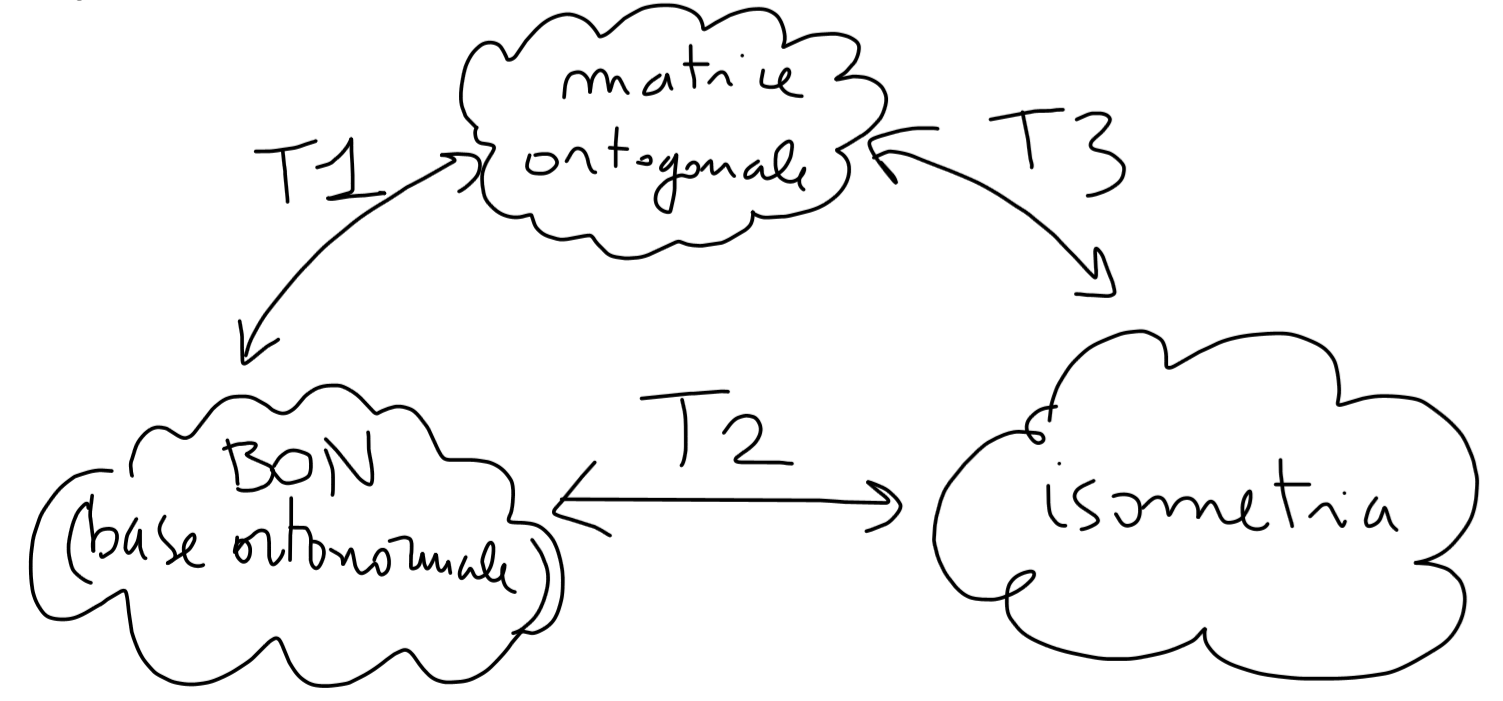
\includegraphics[width=\linewidth]{images/legami_teoremi_isometrie.png}
	\end{center}

	\begin{es}
		$V = \mathbb{R}^3$ con il prodotto scalare standard. $f: V \to V$ definita da $f(x, y, z) = (z, -x, y)$. $f$ è un'isometria?
		\begin{description}
			\item[Soluzione 1] Calcoliamo le norme: $||(x, y, z)|| = \sqrt{x^2 + y^2 + z^2} = \sqrt{z^2 + x^2 + y^2} = ||(z, -x, y)||$. Quindi $f$ è un'isometria.
			\item[Soluzione 2] $f$ manda la base ortonormale $e_1, e_2, e_3$ in $f(e_1) = (0, -1, 0) = -e_2, f(e_2) = (0, 0, 1) = e_3, f(e_3) = (1, 0, 0) = e_1$ che è una base ortonormale di $V$.
			Quindi $f$ è un'isometria per il teorema T2.
			\item[Soluzione 3] La matrice di $f$ rispetto alla base ortonormale $e_1, e_2, e_3$ è: \\
			\[ A = \begin{pmatrix}
				0 & 0 & 1 \\
				-1 & 0 & 0 \\
				0 & 1 & 0
			\end{pmatrix} \]
			Calcoliamo $A^TA = \begin{pmatrix}
				0 & -1 & 0 \\
				0 & 0 & 1 \\
				1 & 0 & 0
			\end{pmatrix} \begin{pmatrix}
				0 & 0 & 1 \\
				-1 & 0 & 0 \\
				0 & 1 & 0
			\end{pmatrix} = \begin{pmatrix}
				1 & 0 & 0 \\
				0 & 1 & 0 \\
				0 & 0 & 1
			\end{pmatrix} = I_3$. \\
			Quindi $f$ è un'isometria per il teorema T3.
		\end{description}
	\end{es}

	\begin{es}
		$V = \mathbb{R}^2$ con il prodotto scalare standard. \\
		$f: V \to V$ definita da $f(x, y, z) = (z, x, y)$. $f$ è un'isometria? \\
		Sì perchè $||(x, y, z)|| = \sqrt{x^2 + y^2 + z^2} = \sqrt{z^2 + x^2 + y^2} = ||(z, x, y)||$.
	\end{es}

	\begin{es}
		Dimostrare che se due matrici $A, M$ sono congruenti, allora i loro determinanti hanno lo stesso segno. \\
		Se $A$ e $M$ sono congruenti, allora esiste una matrice invertibile $B$ tale che $M = B^tAB$. \\
		Allora $\det(M) = \det(B^tAB) = \det(B^t)\det(A)\det(B) = (\det(B))^2\det(A)$. \\
		Ma $(\det(B))^2 \ge 0$ e quindi $\det(M)$ e $\det(A)$ hanno lo stesso segno.
	\end{es}

	\begin{oss}
		In particolare, la matrice di un prodotto scalare deve avere determinante positivo, perchè è congruente alla matrice $I_n$ per il teorema di Sylvester.
	\end{oss}

	\paragraph{Esempio TEST esame}
	Data $a_1v_1 + a_2v_2 + a_3v_3 = 0$ è vero che l'unica soluzione è $a_1 = a_2 = a_3 = 0$? \\
	\textbf{No, non è vero.} Infatti, se $v_1, v_2, v_3$ sono linearmente indipendenti, allora l'unica soluzione è $a_1 = a_2 = a_3 = 0$. \\
	Se invece sono linearmente dipendenti, allora esistono $a_1, a_2, a_3 \in \mathbb{R}$ tali che $a_1v_1 + a_2v_2 + a_3v_3 = 0$ con almeno uno tra $a_1, a_2, a_3$ diverso da zero.
\end{document}
